\documentclass[12pt,openany]{book}

%FIXME: for PRINT run for lulu or kdp, search for %PRINT

%\usepackage{pdf14}

\usepackage[shortlabels]{enumitem}
\usepackage{ifpdf}
\usepackage[shortalphabetic,msc-links]{amsrefs}
\usepackage{mathtools}
\usepackage{amsmath}
\usepackage{amsfonts}
\usepackage{amssymb}
\usepackage{amsthm}
\usepackage{graphicx}
\usepackage{xcolor}
\usepackage{lipsum}
\usepackage{chngcntr}
\usepackage{titlesec}
\usepackage{import}
\usepackage{vogtwidebar}
\usepackage{nicefrac}
\usepackage{mathdots}
\usepackage{microtype}
\usepackage{cancel}
\usepackage{framed}
\usepackage{import}
\usepackage{varioref}

\usepackage{perpage}

\usepackage{tikz}
\usetikzlibrary{cd}
\usepackage{rotating}

\usepackage{cellspace}
\usepackage[toc,nopostdot,sort=use,nomain,automake]{glossaries}

%Palatino
\usepackage[theoremfont]{newpxtext}
\usepackage[vvarbb]{newpxmath}
\linespread{1.05}
\usepackage[scr=boondoxo]{mathalfa} % but we want the nice fancy script fonts

\usepackage[T1]{fontenc}

%symmetric for web
\usepackage[inner=1.2in,outer=1.2in,top=1in,bottom=1in]{geometry}
%PRINT asymetric for book
%\usepackage[inner=1.3in,outer=1.1in,top=1in,bottom=1in]{geometry}

%\newcommand{\mytitleparbox}[1]{\parbox[t]{0.9\textwidth}{\filleft {#1}}}
%\titleformat{\chapter}[hang]{\Huge\bfseries}{\thechapter$i$}{20pt}%
%{\hfill\mytitleparbox}%
%[\vspace{-1ex}\rule{0.5\textwidth}{0.5pt}\rule{0.5\textwidth}{1pt}]

\usepackage[margin=10pt,font=small,labelfont=bf,labelsep=colon,singlelinecheck=false]{caption}

%FIXME: this is nonsense, this should be done above, except maybe the
%cutting down

% smaller margins top/bottom margins
%\addtolength{\textheight}{0.8in}
%\addtolength{\topmargin}{-0.3in}

%thinner text
%\addtolength{\textheight}{0.8in}

%PRINT
%First offset even/odd pages a bit
% not for the coil bound full letter size one
%\addtolength{\oddsidemargin}{0.2in}
%\addtolength{\evensidemargin}{-0.2in}

%PRINT
%Now cut page size a bit.  I'll run it through ghostcript anyway
%to convert to the right size, but this is good for crown quatro
%conversion, don't use for the full letter size versions
%\addtolength{\paperwidth}{-0.3in}
%\addtolength{\paperheight}{-1in}
%\addtolength{\topmargin}{-0.5in}
%\addtolength{\oddsidemargin}{-0.15in}
%\addtolength{\evensidemargin}{-0.15in}


\usepackage{url}
\usepackage{imakeidx}
\PassOptionsToPackage{hyphens}{url}
\usepackage{hyperref} % do NOT set [ocgcolorlinks] here!

%If you have an older tex installation you might need
%to comment out the next line:
%PRINT (COMMENT OUT FOR PRINT)
\usepackage[ocgcolorlinks]{ocgx2} %perhaps run without for lulu/kdp

\usepackage[all]{hypcap}

%\usepackage{draftwatermark}
%\SetWatermarkText{Draft of v3.0 as of \today. May change substantially!}
%\SetWatermarkAngle{90}
%\SetWatermarkHorCenter{0.5in}
%\SetWatermarkColor[gray]{0.7}
%\SetWatermarkScale{0.18}

\definecolor{gray75}{gray}{0.75}

\titleformat{\chapter}[hang]{\Huge\bfseries\filleft}%
{\thechapter$i$\hspace*{10pt}{\textcolor{gray75}{$\backslash\!\!\backslash$}}}%
{10pt}%
{}
[\vspace{-1ex}\rule{0.5\textwidth}{0.5pt}\rule{0.5\textwidth}{1pt}]

\titleformat{\section}[hang]{\Large\bfseries}%
{\thesection$i$\hspace*{10pt}{\textcolor{gray75}{$\backslash$}}}%
{10pt}%
{}%

\titleformat{\subsection}[hang]{\large\bfseries}%
{\thesubsection$i$\hspace*{10pt}{\textcolor{gray75}{$\cdot$}}}%
{10pt}%
{}%

\assignpagestyle{\chapter}{empty}


% Footnotes should use symbols, not numbers.  Numbered footnotes are
% evil, not using footmisc as it conflicts with hyperref
%\usepackage[perpage,symbol*]{footmisc}

% The [2] would not use star
%\MakePerPage[2]{footnote}
\MakePerPage{footnote}
\renewcommand{\thefootnote}{\fnsymbol{footnote}}


% useful
\newcommand{\ignore}[1]{}

% analysis/geometry stuff
\newcommand{\ann}{\operatorname{ann}}
\renewcommand{\Re}{\operatorname{Re}}
\renewcommand{\Im}{\operatorname{Im}}
\newcommand{\Orb}{\operatorname{Orb}}
\newcommand{\hol}{\operatorname{hol}}
\newcommand{\aut}{\operatorname{aut}}
\newcommand{\Aut}{\operatorname{Aut}}
\newcommand{\codim}{\operatorname{codim}}
\newcommand{\sing}{\operatorname{sing}}
\newcommand{\ord}{\operatorname{ord}}
\newcommand{\dist}{\operatorname{dist}}
\newcommand{\Arg}{\operatorname{Arg}}

% reals
\newcommand{\esssup}{\operatorname{ess~sup}}
\newcommand{\essran}{\operatorname{essran}}
\newcommand{\innprod}[2]{\langle #1 | #2 \rangle}
\newcommand{\linnprod}[2]{\langle #1 , #2 \rangle}
\newcommand{\blinnprod}[2]{\bigl\langle #1 , #2 \bigr\rangle}
\newcommand{\supp}{\operatorname{supp}}
\newcommand{\Nul}{\operatorname{Nul}}
\newcommand{\Ran}{\operatorname{Ran}}
\newcommand{\sabs}[1]{\lvert {#1} \rvert}
\newcommand{\snorm}[1]{\lVert {#1} \rVert}
\newcommand{\babs}[1]{\bigl\lvert {#1} \bigr\rvert}
\newcommand{\bnorm}[1]{\bigl\lVert {#1} \bigr\rVert}
\newcommand{\Babs}[1]{\Bigl\lvert {#1} \Bigr\rvert}
\newcommand{\Bnorm}[1]{\Bigl\lVert {#1} \Bigr\rVert}
\newcommand{\bbabs}[1]{\biggl\lvert {#1} \biggr\rvert}
\newcommand{\bbnorm}[1]{\biggl\lVert {#1} \biggr\rVert}
\newcommand{\BBabs}[1]{\Biggl\lvert {#1} \Biggr\rvert}
\newcommand{\BBnorm}[1]{\Biggl\lVert {#1} \Biggr\rVert}
\newcommand{\abs}[1]{\left\lvert {#1} \right\rvert}
\newcommand{\norm}[1]{\left\lVert {#1} \right\rVert}

% sets (some)
\newcommand{\C}{{\mathbb{C}}}
\newcommand{\R}{{\mathbb{R}}}
\newcommand{\Z}{{\mathbb{Z}}}
\newcommand{\N}{{\mathbb{N}}}
\newcommand{\Q}{{\mathbb{Q}}}
\newcommand{\D}{{\mathbb{D}}}
\newcommand{\F}{{\mathbb{F}}}

% consistent
\newcommand{\bB}{{\mathbb{B}}}
\newcommand{\bC}{{\mathbb{C}}}
\newcommand{\bR}{{\mathbb{R}}}
\newcommand{\bZ}{{\mathbb{Z}}}
\newcommand{\bN}{{\mathbb{N}}}
\newcommand{\bQ}{{\mathbb{Q}}}
\newcommand{\bD}{{\mathbb{D}}}
\newcommand{\bF}{{\mathbb{F}}}
\newcommand{\bH}{{\mathbb{H}}}
\newcommand{\bO}{{\mathbb{O}}}
\newcommand{\bP}{{\mathbb{P}}}
\newcommand{\bK}{{\mathbb{K}}}
\newcommand{\bV}{{\mathbb{V}}}
\newcommand{\CP}{{\mathbb{CP}}}
\newcommand{\RP}{{\mathbb{RP}}}
\newcommand{\HP}{{\mathbb{HP}}}
\newcommand{\OP}{{\mathbb{OP}}}
\newcommand{\sA}{{\mathscr{A}}}
\newcommand{\sB}{{\mathscr{B}}}
\newcommand{\sC}{{\mathscr{C}}}
\newcommand{\sF}{{\mathscr{F}}}
\newcommand{\sG}{{\mathscr{G}}}
\newcommand{\sH}{{\mathscr{H}}}
\newcommand{\sM}{{\mathscr{M}}}
\newcommand{\sO}{{\mathscr{O}}}
\newcommand{\sP}{{\mathscr{P}}}
\newcommand{\sQ}{{\mathscr{Q}}}
\newcommand{\sR}{{\mathscr{R}}}
\newcommand{\sS}{{\mathscr{S}}}
\newcommand{\sI}{{\mathscr{I}}}
\newcommand{\sL}{{\mathscr{L}}}
\newcommand{\sK}{{\mathscr{K}}}
\newcommand{\sU}{{\mathscr{U}}}
\newcommand{\sV}{{\mathscr{V}}}
\newcommand{\sX}{{\mathscr{X}}}
\newcommand{\sY}{{\mathscr{Y}}}
\newcommand{\sZ}{{\mathscr{Z}}}
\newcommand{\fS}{{\mathfrak{S}}}

\newcommand{\interior}{\operatorname{int}}

% Topo stuff
\newcommand{\id}{\textit{id}}
\newcommand{\im}{\operatorname{im}}
\newcommand{\rank}{\operatorname{rank}}
\newcommand{\Tor}{\operatorname{Tor}}
\newcommand{\Torsion}{\operatorname{Torsion}}
\newcommand{\Ext}{\operatorname{Ext}}
\newcommand{\Hom}{\operatorname{Hom}}

%extra thingies
%\newcommand{\mapsfrom}{\ensuremath{\text{\reflectbox{$\mapsto$}}}}
\newcommand{\from}{\ensuremath{\leftarrow}}
\newcommand{\dhat}[1]{\hat{\hat{#1}}}

\definecolor{mypersianblue}{rgb}{0.11, 0.22, 0.73}

\hypersetup{
    pdfborderstyle={/S/U/W 0.5}, %this just in case ocg isn't there
    %PRINT (for print use the below and comment out the above):
    %pdfborder={0 0 0},
    citecolor=mypersianblue,
    filecolor=mypersianblue,
    linkcolor=mypersianblue,
    urlcolor=mypersianblue,
    pdftitle={Guide to Cultivating Complex Analysis},
    pdfsubject={Complex Analysis},
    pdfkeywords={one complex variable, complex analysis},
    pdfauthor={Jiri Lebl}
}

% Set up our index
\makeindex

% Very simple indexing
\newcommand{\myindex}[1]{#1\index{#1}}

\author{Ji\v{r}\'i Lebl}

\title{Guide to Cultivating Complex Analysis}

% Don't include subsections
\setcounter{tocdepth}{1}

\theoremstyle{plain}
\newtheorem{thm}{Theorem}[section]
\newtheorem{lemma}[thm]{Lemma}
\newtheorem{prop}[thm]{Proposition}
\newtheorem{cor}[thm]{Corollary}
\newtheorem{claim}[thm]{Claim}

\theoremstyle{remark}
\newtheorem{remark}[thm]{Remark}

\theoremstyle{definition}
\newtheorem{defn}[thm]{Definition}

\newtheoremstyle{exercise}% name
  {}% Space above
  {}% Space below
  {\itshape}% Body font
  {}% Indent amount 1
  {\bfseries \itshape}% Theorem head font
  {:}% Punctuation after theorem head
  {.5em}% Space after theorem head 2
  {}% Theorem head spec (can be left empty, meaning "normal")

\newenvironment{exbox}{%
    \def\FrameCommand{\vrule width 1pt \relax\hspace {10pt}}%
    \MakeFramed {\advance \hsize -\width \FrameRestore }%
}{%
    \endMakeFramed
}

\newenvironment{exparts}{%
    \leavevmode\begin{enumerate}[a),noitemsep,topsep=0pt,parsep=0pt,partopsep=0pt]
}{%
    \end{enumerate}
}
\newenvironment{exnumparts}{%
    \leavevmode\begin{enumerate}[1),noitemsep,topsep=0pt,parsep=0pt,partopsep=0pt]
}{%
    \end{enumerate}
}

\newenvironment{myfig}{%
\begin{figure}[h!t]
\noindent\rule{\textwidth}{0.4pt}\vspace{12pt}\par\centering}%
{\par\noindent\rule{\textwidth}{0.4pt}
\end{figure}}


\newenvironment{myquote}{%
    \begin{quote}%
    %\begin{center}%
    \begingroup\itshape
}{%
    \endgroup%
    %\end{center}%
    \end{quote}
}

\theoremstyle{exercise}
\newtheorem{exercise}{Exercise}[section]

\newtheoremstyle{example}% name
  {}% Space above
  {}% Space below
  {}% Body font
  {}% Indent amount 1
  {\bfseries}% Theorem head font
  {:}% Punctuation after theorem head
  {.5em}% Space after theorem head 2
  {}% Theorem head spec (can be left empty, meaning "normal")

\theoremstyle{example}
\newtheorem{example}[thm]{Example}

% referencing
\newcommand{\figureref}[1]{\hyperref[#1]{Figure~\ref*{#1}}}
\newcommand{\tableref}[1]{\hyperref[#1]{Table~\ref*{#1}}}
\newcommand{\chapterref}[1]{\hyperref[#1]{chapter~\ref*{#1}}}
\newcommand{\Chapterref}[1]{\hyperref[#1]{Chapter~\ref*{#1}}}
\newcommand{\appendixref}[1]{\hyperref[#1]{appendix~\ref*{#1}}}
\newcommand{\Appendixref}[1]{\hyperref[#1]{Appendix~\ref*{#1}}}
\newcommand{\sectionref}[1]{\hyperref[#1]{section~\ref*{#1}}}
\newcommand{\exerciseref}[1]{\hyperref[#1]{Exercise~\ref*{#1}}}
\newcommand{\exampleref}[1]{\hyperref[#1]{Example~\ref*{#1}}}
\newcommand{\thmref}[1]{\hyperref[#1]{Theorem~\ref*{#1}}}
\newcommand{\propref}[1]{\hyperref[#1]{Proposition~\ref*{#1}}}
\newcommand{\lemmaref}[1]{\hyperref[#1]{Lemma~\ref*{#1}}}
\newcommand{\corref}[1]{\hyperref[#1]{Corollary~\ref*{#1}}}
\newcommand{\defnref}[1]{\hyperref[#1]{Definition~\ref*{#1}}}

% List of Symbols/Notation
\newglossary[nlg]{notation}{not}{ntn}{List of Notation}

\loadglsentries{notations}
\makeglossaries

\begin{document}

\ifpdf
  \pdfbookmark{Title Page}{title}
\fi
\newlength{\centeroffset}
\setlength{\centeroffset}{-0.5\oddsidemargin}
\addtolength{\centeroffset}{0.5\evensidemargin}
%\addtolength{\textwidth}{-\centeroffset}
\thispagestyle{empty}
\vspace*{\stretch{1}}
\noindent\hspace*{\centeroffset}\makebox[0pt][l]{\begin{minipage}{\textwidth}
\flushright
{\Huge\bfseries \sffamily Guide to Cultivating Complex Analysis}
\noindent\rule[-1ex]{\textwidth}{5pt}\\[2.5ex]
\hfill\emph{\Large \sffamily Indoctrination in One Variable}
\end{minipage}}

\vspace{\stretch{1}}
\noindent\hspace*{\centeroffset}\makebox[0pt][l]{\begin{minipage}{\textwidth}
\flushright
{\bfseries 
%by
Ji{\v r}\'i Lebl\\[3ex]} 
\today
\\
(version 0.0)
\end{minipage}}

%\addtolength{\textwidth}{\centeroffset}
\vspace{\stretch{2}}


\pagebreak

\vspace*{\fill}

%\begin{small} 
\noindent
Typeset in \LaTeX.

\bigskip

\noindent
Copyright \copyright 2019 Ji{\v r}\'i Lebl

%PRINT
% not for the coil version
%\noindent
%ISBN 978-0-359-64225-0

\bigskip

%\begin{floatingfigure}{1.4in}
%\vspace{-0.05in}
\noindent

\includegraphics[width=1.38in]{figures/license}
\quad

\includegraphics[width=1.38in]{figures/license2}
%\end{floatingfigure}

\bigskip

\noindent
\textbf{License:}
\\
This work is dual licensed under
the Creative Commons
Attribution-Non\-commercial-Share Alike 4.0 International License and
the Creative Commons
Attribution-Share Alike 4.0 International License.
To view a
copy of these licenses, visit
\url{https://creativecommons.org/licenses/by-nc-sa/4.0/}
or
\url{https://creativecommons.org/licenses/by-sa/4.0/}
or send a letter to
Creative Commons
PO Box 1866, Mountain View, CA 94042, USA\@.
%Creative Commons, 171 Second Street, Suite 300, San Francisco, California,
%94105, USA.

\bigskip

\noindent
You can use, print, duplicate, share this book as much as you want.  You can
base your own notes on it and reuse parts if you keep the license the
same.  You can assume the license is either the CC-BY-NC-SA or CC-BY-SA\@,
whichever is compatible with what you wish to do, your derivative works must
use at least one of the licenses.

%\bigskip
%
%\noindent
%\textbf{Acknowledgments:}
%\\
%I would like to thank FIXME
%and students in my classes for pointing out typos/errors
%and helpful suggestions. 
%
%\bigskip
%
%\noindent
%During the writing of this book, 
%the author was in part supported by NSF grant DMS-1362337.

\bigskip

\noindent
\textbf{More information:}
\\
See \url{https://www.jirka.org/ca/} for more information
(including contact information).

\medskip

\noindent
The \LaTeX\ source for the book is available
for possible modification and customization
at github: \url{https://github.com/jirilebl/ca}


% For large print do this
%\large

\microtypesetup{protrusion=false}
\tableofcontents
\microtypesetup{protrusion=true}

%\addtocontents{toc}{\protect\vspace{-2\baselineskip}}
%\addtocontents{toc}{\protect\vspace{-\baselineskip}}
%\addtocontents{toc}{\protect\enlargethispage{\baselineskip}}

%%%%%%%%%%%%%%%%%%%%%%%%%%%%%%%%%%%%%%%%%%%%%%%%%%%%%%%%%%%%%%%%%%%%%%%%%%%%%%
%%%%%%%%%%%%%%%%%%%%%%%%%%%%%%%%%%%%%%%%%%%%%%%%%%%%%%%%%%%%%%%%%%%%%%%%%%%%%%
%%%%%%%%%%%%%%%%%%%%%%%%%%%%%%%%%%%%%%%%%%%%%%%%%%%%%%%%%%%%%%%%%%%%%%%%%%%%%%

\chapter*{Introduction} \label{ch:intro}
\addcontentsline{toc}{chapter}{Introduction}
\markboth{INTRODUCTION}{INTRODUCTION}

\begin{myquote}
Let us be thankful for the fools. But for them the rest of us could not succeed.

---Mark Twain 
\end{myquote}

The purpose of this book is to teach a one-semester graduate course in
complex analysis.
It is a natural first semester in a two semester sequence where the second
semester could be several complex variables or perhaps harmonic analysis.
What is assumed is basic knowledge of undergraduate
analysis in the real variable, called advanced calculus in some schools.
The text assumes knowledge of metric spaces
and differential analysis in several variables, but if the reader is not
confident on these topics or has not yet seen them, the useful results
are presented in the appendices.  With that, basic prerequisite for the
course could be a single semester of undergraduate analysis if the
appendices are also covered.  Very basic linear algebra and abstract algebra
is also useful.

This book takes the view that we do not need to redefine and reprove
things that we have done in a basic real analysis course, especially with
regards to mappings of the plane.  We can quite quickly jump to
holomorphic functions as solutions of the Cauchy--Riemann equations for
example.
The connection is to understand multiplication by complex numbers
as a $2 \times 2$ real matrix.
Similarly, when we introduce line integrals we connect
them to the line integrals the student has seen in calculus.
This is not simply a time saving measure.
The point is to stress that we are not defining some totally new and different world.

We also want to take a more of the $z,\bar{z}$ approach and less the
$x,y$ approach.  It is really a better way to think about complex variables,
although perhaps initially less intuitive.

Furthermore, we try not to define any conflicting terminology or notation
with what the reader has learned before.
Mainly, the term ``differentiable'' is generally left for the real
derivative and we use ``complex differentiable'' when needed.  Although
to be sure, 
we will generally write ``(real) differentiable'' or
``differentiable (in the real sense)'' to
make it clear when we mean real differentiability.

%%%%%%%%%%%%%%%%%%%%%%%%%%%%%%%%%%%%%%%%%%%%%%%%%%%%%%%%%%%%%%%%%%%%%%%%%%%%%%
%%%%%%%%%%%%%%%%%%%%%%%%%%%%%%%%%%%%%%%%%%%%%%%%%%%%%%%%%%%%%%%%%%%%%%%%%%%%%%
%%%%%%%%%%%%%%%%%%%%%%%%%%%%%%%%%%%%%%%%%%%%%%%%%%%%%%%%%%%%%%%%%%%%%%%%%%%%%%

\chapter{The Complex Plane} \label{ch:complexplane}

\begin{myquote}
It's clearly a budget. It's got a lot of numbers in it.

---George W.\ Bush
\end{myquote}

%%%%%%%%%%%%%%%%%%%%%%%%%%%%%%%%%%%%%%%%%%%%%%%%%%%%%%%%%%%%%%%%%%%%%%%%%%%%%%

\section{Complex numbers} \label{sec:complexnums}

%In modern mathematics, in other words in the last couple hundred years, when 
%faced with a problem such as solving $z^2+1 = 0$,
%instead of trying to see when the equation has a solution with
%the numbers we have, we define new numbers that solve the equation.

Modern\footnote{In this context \emph{modern}
means ``later than the middle ages.''}
mathematics
is taking a false statement such as ``all
polynomials have a root'' and redefining what we mean by a ``number,''
so that the statement is true.  In this case we arrive at the complex
numbers.  Surprisingly, while this technique
just feels like cheating, it has been very productive in giving us
essentially all the mathematics we know, both pure and applied.  It is this same
technique that starts with the natural numbers
\glsadd{not:N}$\N = \{ 1,2,3,\ldots \}$, which are the only
numbers that we can really make an argument are obvious from nature,
and gets us zero and the negative numbers producing the integers
\glsadd{not:Z}$\Z$ so that we can solve equations such as $n+2 = 1$.
From \glsadd{not:Z}$\Z$, we define the rational numbers
\glsadd{not:Z}$\Q$ to solve equations such as $2x=1$.  We extend
\glsadd{not:Z}$\Q$ to the real numbers \glsadd{not:R}$\R$
to solve equations such as $x^2=2$.  Really we want the real numbers to
have things like the Intermediate Value Theorem, Bolzano--Weierstrass,
etc.  It is then not much of a stretch to do the same thing when trying
to solve $z^2+1=0$.  Similarly as what happened when we defined the real
numbers, the consequences of adding this solution to the mix are much more
profound than just finding roots of polynomials.

\subsection{The complex numbers as the plane}

You have surely seen the complex number field,
but let us review how one can define it.
As a set, let the \emph{\myindex{complex number field}}
\glsadd{not:C}$\C$ be the set $\R^2 = \R \times \R$.
As the set is a plane, we call it the \emph{\myindex{complex plane}}%
\footnote{Although there is that odd mathematician out there that
thinks that the \emph{complex plane} is $\C^2 = \C \times \C$.
If you hear someone say that, politely whack them over the head for me.}.
To make it a field, we define addition and product:
\begin{align*}
(a,b) + (c,d) & \overset{\text{def}}{=} (a+b,c+d) , \\
(a,b) (c,d) & \overset{\text{def}}{=} (ac-bd,bc+da) .
\end{align*}

\begin{exbox}
\begin{exercise}
Check that the above makes $\C$ into a field, where the additive
identity $0=(0,0)$ and the multiplicative is $1=(1,0)$.
That is, it is an abelian group under addition,
the nonzero complex numbers are an abelian group under multiplication,
and the distributive law holds.  Hint: The multiplicative inverse of $(a,b)$
is $\left(\frac{a}{a^2+b^2},\frac{-b}{a^2+b^2}\right)$.
\end{exercise}
\end{exbox}

We will actually never write complex numbers as $(x,y)$ from now on.
When we write a real number $x$ we identify it with the
complex number $(x,0)$.
With this identification $\R \subset \C$.
We also define the \emph{\myindex{imaginary unit}}%
\footnote{Beware of engineers, they think it is called $j$, despite there
being no ``j'' in ``imaginary.''}%
\glsadd{not:i}
\begin{equation*}
i \overset{\text{def}}{=} (0,1) ,
\end{equation*}
and we find that with this definition $(x,y) = x+iy$, using the field
structure of $\C$.  So from now on, this is the only way we write
the complex numbers.  We call the form $x+iy$ the \emph{\myindex{cartesian}}
form of the complex number.

The number $i$ has the magical property that
\begin{equation*}
i^2 = 1 .
\end{equation*}
It is the solution to $z^2+1=0$.
For this reason we sometimes%
\footnote{There are those that \emph{always} write $\sqrt{-1}$ instead of $i$.
Those people also deserve a good whack.}
write $i = \sqrt{-1}$.
We will prove later that complex numbers
are precisely the field in which every polynomial has roots.
Note that there is another square root of $-1$, that is $-i$.

%\begin{remark}
%Another way to define complex numbers is to take the real numbers
%and adjoin a root of $z^2+1=0$.
%There is a subtle philosophical issue with the fact that there
%are two such square roots.
%Two chickens\index{chicken!imaginary}%
%are running around in our yard,
%and because we like to
%know which is which, we catch one and write ``$i$'' on it.  If we happened
%to have caught the other chicken, we would have gotten an exactly equivalent
%theory, which we could not tell apart from the original.
%\end{remark}

Given a complex number $z$, its ``evil twin'' is 
the \emph{\myindex{complex conjugate}} of $z$ and is defined as
\glsadd{not:conj}%
\begin{equation*}
\bar{z} \overset{\text{def}}{=} x-iy.
\end{equation*}

If $z = x+iy \in \C$ for $x,y \in \R$, then $x$ is called the
\emph{\myindex{real part}} and $y$ is called the
\emph{\myindex{imaginary part}}.  We write
\glsadd{not:real}%
\glsadd{not:imag}%
\begin{equation*}
\Re z = 
\Re (x+iy) =
\frac{z+\bar{z}}{2}
= x, \qquad 
\Im z = 
\Im (x+iy) =
\frac{z-\bar{z}}{2i}
=
y .
\end{equation*}
A particularly useful observation one can make is that above we wrote the
real part and the imaginary part in terms of $z$ and $\bar{z}$.
Any expression we write in the real and imaginary parts of $z$ we can
equally well write in terms of $z$ and $\bar{z}$, and vice-versa.
For example,
\begin{equation*}
x^3 + y^3 + 3ixy
=
{\left( \frac{z+ \bar{z}}{2} \right)}^3 + 
{\left( \frac{z- \bar{z}}{2i} \right)}^3 + 
3i {\left( \frac{z+ \bar{z}}{2} \right)} 
{\left( \frac{z- \bar{z}}{2i} \right)} ,
\end{equation*}
or
\begin{equation*}
z^2 - i \bar{z}^2 + z \bar{z}
=
{(x+iy)}^2 - i {(x-iy)}^2 + 
(x+iy)(x-iy) .
\end{equation*}
It may seem that an expression in terms of $z$ and $\bar{z}$ is more
complicated.  In particular, $z$ and $\bar{z}$ are not
``independent variables.''  However, it is particularly powerful to
think in terms of $z$ and $\bar{z}$ instead of $x$ and $y$, and to pretend
in many contexts as if $z$ and $\bar{z}$ were actually independent
variables.

\subsection{The geometry and topology of the plane}


The size of $z$ is measured by the so-called \emph{\myindex{modulus}},
which is just the \emph{\myindex{Euclidean distance}}:
\glsadd{not:mod}%
\begin{equation*}
\sabs{z} \overset{\text{def}}{=} \sqrt{z \bar{z}} = \sqrt{x^2+y^2} .
\end{equation*}
Perhaps easier and more useful equation is ${\sabs{z}}^2 = z\bar{z}$.
Notice $\sabs{z} \geq 0$, and $\sabs{z} = 0$
if and only if $z=0$.

\begin{prop}[Cauchy--Schwarz and the triangle inequality]
If $z,w \in \C$, then
\begin{enumerate}[(i)]
\item
$\Re z\bar{w} \leq \sabs{z} \sabs{w}$ \quad (Cauchy--Schwarz),
\item
$\sabs{z+w} \leq \sabs{z} + \sabs{w}$ \quad (Triangle inequality).
\end{enumerate}
\end{prop}

\begin{proof}
The modulus squared of a complex number is always nonnegative:
\begin{equation*}
\begin{split}
0 & \leq {\sabs{z\bar{w}-\bar{z}w}}^2 \\
  & =    (z\bar{w}-\bar{z}w)(z\bar{w}-\bar{z}w) \\
  & =    2z\bar{z}w\bar{w} - z^2\bar{w}^2 - \bar{z}^2w^2 \\
  & =    4z\bar{z}w\bar{w} - {(z\bar{w}+\bar{z}w)}^2 \\
  & =    {(2\sabs{z}\sabs{w})}^2 - {(2 \Re z\bar{w})}^2 .
\end{split}
\end{equation*}
This proves Cauchy--Schwarz.  We prove the triangle inequality
via Cauchy--Schwarz:
\begin{equation*}
\begin{split}
{\sabs{z+w}}^2 & =    (z+w)(\bar{z}+\bar{w}) \\
               & =    z\bar{z} + w\bar{w} + z\bar{w} + \bar{z}w \\
               & \leq z\bar{z} + w\bar{w} + 2 \sabs{z}\sabs{w} \\
               & =    {(\sabs{z}+\sabs{w})}^2 . \qedhere
\end{split}
\end{equation*}
\end{proof}

\begin{exbox}
\begin{exercise}
Prove the polarization identity
$4 z\bar{w} =
{\sabs{z+w}}^2-{\sabs{z-w}}^2 +i \bigl( {\sabs{z+iw}}^2 - {\sabs{z-iw}}^2 \bigr)$.
\end{exercise}
\end{exbox}

The distance between two numbers $z$ and $w$ is measured by
\begin{equation*}
%\dist(z,w)
%\overset{\text{def}}{=}
\sabs{z-w} ,
\end{equation*}
and this makes $\C$ into a metric space.  See \Appendixref{ap:metric}
for an introduction to metric spaces.

\begin{exbox}
\begin{exercise}
Prove that complex addition, multiplication, and division is continuous.
That is, suppose $\{ a_n \}$ and $\{ b_n \}$ are two convergent sequences
of complex numbers.  Prove (including the existence of the limits)
\begin{exparts}
\item
$\lim\limits_{n\to\infty} (a_n + b_n) = 
\left(\lim\limits_{n\to\infty} a_n \right) +
\left(\lim\limits_{n\to\infty} b_n \right)$.
\item
$\lim\limits_{n\to\infty} a_n b_n = 
\left(\lim\limits_{n\to\infty} a_n \right)
\left(\lim\limits_{n\to\infty} b_n \right)$.
\item
If $\lim\limits_{n\to\infty} a_n \not= 0$, then
$\lim\limits_{n\to\infty} \frac{1}{a_n} = \frac{1}{\lim\limits_{n\to\infty}
a_n}$.
\end{exparts}
\end{exercise}
\end{exbox}

The basic neighborhood (that is, an
open ball) in $\C$
is called a \emph{\myindex{disc}}.
Given $a \in \C$ and $\rho > 0$, define the disc of radius $\rho$ around
$a$
as
\glsadd{not:disc}%
\begin{equation*}
\Delta_\rho(a)
\overset{\text{def}}{=}
\bigl\{ z \in \C : \sabs{z-a} < \rho \bigr\} .
\end{equation*}
A disc centered at the origin of radius 1 is called the
\emph{\myindex{unit disc}}
\glsadd{not:D}%
\begin{equation*}
\D
\overset{\text{def}}{=}
\Delta_1(0)
=
\bigl\{ z \in \C : \sabs{z} < 1 \bigr\} .
\end{equation*}
The unit disc will come up often in this course, as it turns out that
a lot of complex analysis can be done by looking at just the unit disc.

The following definition is perhaps somewhat unnecessary, but it is so much
easier to write and say than \emph{open and connected}, and it is commonly
used in complex analysis.

\begin{defn}
An open and connected set $U \subset \C$ is called a
\emph{\myindex{domain}}.
\end{defn}

\subsection{Complex-valued functions}

It is possible that the analysis you have seen so far in your mathematical
career has been for real-valued functions $f \colon X \to \R$.  In this
book, we are concerned with complex-valued functions $f \colon X \to \C$.
The results for real-valued functions are then applied by thinking of
either the components of $f$ separately or by thinking of $\C$ as the
real vector space $\R^2$.

Given a complex-valued function $f \colon X \to \C$ we write $u = \Re f$
and $v = \Im f$ for real-valued functions $u,v \colon X \to \R$, and then
\begin{equation*}
f = u+iv .
\end{equation*}

If $X \subset \C$, then we can think of $X \subset \R^2$.
A derivative in $x$ or $y$ (where $z=x+iy$) is then applied to the
components (as if $f$ was valued in $\R^2$):
\begin{equation*}
\frac{\partial f}{\partial x} = 
\frac{\partial u}{\partial x} + i
\frac{\partial v}{\partial x}
\qquad\text{and}\qquad
\frac{\partial f}{\partial y} = 
\frac{\partial u}{\partial y} + i
\frac{\partial v}{\partial y} .
\end{equation*}

If $X \subset \R$, that is if $f$ is a complex-valued
function of one real variable, $f' = u' + iv'$.
This is equivalent to treating $f$ as a function from $\R$ to $\R^2$
and hence $f'$ is a $2 \times 1$ matrix---a column vector, or in other words
representing a complex number if we are identifying $\C$ and $\R^2$.

Similarly when integrating.  Suppose that $f \colon [a,b] \to \C$.
We say $f$ is (Riemann) integrable if $u$ and $v$ are, and then
\begin{equation*}
\int_a^b f(t) \, dt = 
\int_a^b u(t) \, dt + i \int_a^b v(t) \, dt .
\end{equation*}
Again, this is precisely the way one integrates vector-valued functions
for any vector space.

\subsection{Matrix representation of complex numbers}

As $\C$ is $\R^2$, we can think of
$\C$ as a real two-dimensional vector space by forgetting about the
complex multiplication.  A standard basis is then $1$ and $i$.
To put multiplication back into the picture, we think of an object that
acts on $\R^2$, that is, a matrix.
Complex numbers can also be represented by $2 \times 2$ real matrices.
Represent $x+iy$ as
\begin{equation*}
\begin{bmatrix}
x & -y \\
y & x
\end{bmatrix}
\end{equation*}
If we think of a complex number $a+ib$ as a matrix and $c+id$ as a column vector
then the multiplication
\begin{equation*}
\begin{bmatrix}
a & -b \\
b & a
\end{bmatrix}
\begin{bmatrix}
c \\
d 
\end{bmatrix}
=
\begin{bmatrix}
ac-bd \\
bc+ad .
\end{bmatrix}
\end{equation*}
Note that the matrices
\begin{equation*}
1 \quad ``{}={}'' \quad
\begin{bmatrix}
1 & 0 \\
0 & 1
\end{bmatrix} \qquad \text{and} \qquad
i \quad ``{}={}'' \quad
\begin{bmatrix}
0 & -1 \\
1 & 0
\end{bmatrix} 
\end{equation*}
are the identity and the rotation counterclockwise by 90 degrees
respectively.  Precisely what we expect multiplication by $1$ and $i$
to do.
The complex conjugate is represented by the
matrix transpose, and a symmetric matrix represents a real number.

Of course we can also multiply the $2 \times 2$ matrices themselves,
and this matrix multiplication is also the same as multiplication of complex
numbers.  Similarly with addition.
That is, we can view the field of complex numbers as a subring of $M_2(\R)$.

\begin{exbox}
\begin{exercise}
Prove that the matrix multiplication on these matrices is commutative
and reproduces the complex
number multiplication, and that these matrices form a subring of $M_2(\R)$.
Prove that the nonzero matrices of this form are
invertible (the subring is a field).  In particular, notice the
determinant appearing in the denominator for the multiplicative inverse.
\end{exercise}

\begin{exercise}
Prove that if the $2 \times 2$ matrix $M$ represents a complex number
$a+ib$, then $M$ has two eigenvalues: $a \pm i b$ with the corresponding
eigenvectors $\left[ \begin{smallmatrix} 1 \\ \pm i \end{smallmatrix}
\right]$.
\end{exercise}

\begin{exercise}
Prove that
in terms of the complex notation an arbitrary $2 \times 2$ real matrix $M$
can be represented by two complex numbers $\xi$ and $\zeta$, and the formula
$z \mapsto \xi z + \zeta \bar{z}$.
\end{exercise}
\end{exbox}

We will see this representation of complex numbers come up when we introduce the
Cauchy--Riemann equations.  But it comes up quite often in applications.
This can for example be used to represent an $m \times n$ complex matrix by a
$2m \times 2n$ real matrix by replacing each entry by a $2 \times 2$ matrix.

For us the application will be understand the derivative of a
complex-valued function of a complex variable $f \colon \C \to \C$.
By thinking of the function simply as a mapping $f \colon \R^2 \to \R^2$,
then the real derivative of this mapping is a $2 \times 2$ matrix.  And the
object of study of complex analysis, the holomorphic (or analytic)
functions, are those functions whose real derivative corresponds to a
multiplication by a complex number.

\section{Polar form and the exponential}

\subsection{The exponential}

The exponential is one of the most useful functions in complex analysis
(if not all of analysis).  Let us define it for all complex numbers:
\begin{equation*}
e^{z} = 
e^{x+iy}
\overset{\text{def}}{=}
e^x e^{iy}
=
e^x\cos y + i e^x \sin y .
\end{equation*}
This definition agrees with the standard definition for real numbers (when
$y=0$).  Further note that
\begin{equation*}
e^{\bar{z}} = 
e^{x-iy} =
e^x\cos y - i e^x \sin y  = \overline{e^{z}} ,
\end{equation*}
and
\begin{equation*}
\sabs{e^{z}} = 
\sabs{e^{x-iy}} =
e^x .
\end{equation*}
It is possible to not resort to the real exponentials, sines and cosines
to define the exponential functions, and we will do so in due course.
But we want to have something to play around with already.

\begin{exbox}
\begin{exercise}
Using the definition and trigonometric identities, prove
\begin{equation*}
e^{z+w} = e^z e^w .
\end{equation*}
Remark: In fact, $e^z$ is the unique continuous
function that satisfies the identity above
and also $e^1 = e$, but let us not worry about this now.
\end{exercise}
\end{exbox}

In particular, we have the so-called
\emph{\myindex{Euler's formula}}.  For real $\theta$, the definition
of the exponential says:
\begin{equation*}
e^{i\theta}
=
\cos \theta + i \sin \theta .
\end{equation*}
Using this formula we could extend cosine and sine to the complex plane.
The formula says that for real $\theta$
\begin{equation*}
\cos \theta = \Re e^{i\theta} = \frac{e^{i\theta}+e^{-i\theta}}{2} ,
\qquad
\sin \theta = \Im e^{i\theta} = \frac{e^{i\theta}-e^{-i\theta}}{2i} .
\end{equation*}
We thus simply define cosine and sine for complex numbers by plugging
into that formula, now that we know how to evaluate the exponential:
\begin{equation*}
\cos z \overset{\text{def}}{=} \frac{e^{iz}+e^{-iz}}{2} ,
\qquad
\sin z \overset{\text{def}}{=} \frac{e^{iz}-e^{-iz}}{2i} .
\end{equation*}


\subsection{Polar coordinates}

As complex numbers are just the plane, we could also use polar coordinates
to represent complex numbers.
That is, $x = r \cos \theta$ and $y= r \sin \theta$.  We write this form as
\begin{equation*}
z = x+iy = r e^{i \theta} ,
\end{equation*}
where $r = \sabs{z} = \sqrt{x^2+y^2}$ is the \emph{\myindex{modulus}}, and 
$\theta$ is the angle that $x+iy$ makes with the real axis (the $x$-axis).
The $\theta$ is called the \emph{\myindex{argument}}.  See
\figureref{fig:polarcoords}.

\begin{myfig}
\subimport*{figures/}{polarcoords.pdf_t}
\caption{Polar coordinates.\label{fig:polarcoords}}
\end{myfig}

The reason for the notation is the
Euler's formula, so
\begin{equation*}
z = r e^{i\theta} = r\cos \theta + i r\sin \theta  = x+iy .
\end{equation*}

Polar form is particularly nice for multiplication of numbers and powers.
Suppose $z = r e^{i\theta}$ and $w = s e^{i \psi}$, then
\begin{equation*}
zw =
r e^{i \theta} s e^{i \psi} = 
rs e^{i (\theta+ \psi)},
\qquad
\frac{1}{z} =
\frac{1}{r e^{i \theta}} =
\frac{1}{r} e^{-i \theta} ,
\qquad
z^n =
{\bigl(r e^{i \theta}\bigr)}^n =
r^n e^{i n\theta} .
\end{equation*}
In particular, again we see that multiplication by $i = e^{i \pi / 2}$ is
rotation counterclockwise by 90 degrees.
On the other hand, the polar form is particularly terrible for addition.
You win some, you lose some.

\begin{exbox}
\begin{exercise}
Let $z,w$ be two nonzero complex numbers and let
$\ell_z$ and $\ell_w$ be the lines through the origin and
$z$ and $w$ respectively.  Write $\theta$ for the angle between $\ell_z$ and
$\ell_w$.  Then prove that
$\Re z\bar{w} = \sabs{z} \sabs{w} \cos \theta$.
Note that $\Re z\bar{w}$ is the standard real dot product in $\R^2$, and so
this is the formula for the dot product from calculus.
\end{exercise}
\end{exbox}

\subsection{The argument}

We attempt to define the argument as
\glsadd{not:arg}%
\begin{equation*}
\arg z
\overset{\text{def?}}{=}
\theta ,
\end{equation*}
but we run up against the problem that if $\theta$ is an argument of $z$,
then so is $\theta+2\pi$ or $\theta + k 2\pi$ for any $k$.  In other words,
$\arg z$ is not a function in the classical sense, but a
\emph{\myindex{multivalued function}}%
\footnote{Non-complex analysts will sometimes claim that a multivalued
function is nonsense, but you can safely ignore them.}.  The correct
definition is then
\begin{equation*}
\arg z
\overset{\text{def}}{=}
\ldots,\theta - 4\pi,
\theta - 2\pi,
\theta ,
\theta + 2\pi,
\theta + 4\pi, \ldots
\end{equation*}
There is one more minor issue left.  If $z=0$, then $z=0=0 e^{i\theta}$ for any
$\theta$ whatsoever.  Therefore, we only define the argument for nonzero
$z$.

Sometimes it is useful to nail down a particular number for the argument.
We thus define the \emph{\myindex{principal branch of $\arg$}} as
\begin{equation*}
\Arg z
\overset{\text{def}}{=}
\theta, \qquad \text{where $-\pi < \theta \leq \pi$.}
\end{equation*}
It may seem like a good solution to the multivaluedness of $\arg$, but
one's hopes are dashed by the cruel reality of $\Arg$ not being continuous
on the negative real axis.  The principal branch ends up being somewhat less
useful than we may think.  There is also the issue that not everyone agrees
on what ``principal branch'' means; some mathematicians will sacrifice the
positive real axis and let $\theta$ be in the range $[0,2\pi)$.

\subsection{Mapping properties of the exponential}

Before we leave the exponential, let us note what it does to the complex
plane.  First, the identity $e^{z+w} = e^z e^w$ implies that the exponential
can never be zero (exercise).  From known properties of polar coordinates
(so properties of real sine and cosine) it follows that the exponential is
onto $\C \setminus \{ 0 \}$.
The complex exponential is not one-to-one, it is in fact
infinitely-many-to-one.  For any integer $k$
\begin{equation*}
e^{z+ik2\pi} = 
e^{z} e^{ik2\pi} =
e^z .
\end{equation*}

\begin{exbox}
\begin{exercise}
Then prove that those are really the only such identities by
showing that if $2ki\pi < \Im z \leq 2(k+1)i\pi$ and
$2ki\pi < \Im w \leq 2(k+1)i\pi$, then $e^z=e^w$ implies $z=w$.
\end{exercise}
\end{exbox}

Let us consider a vertical line given by $x=c$.  As
\begin{equation*}
e^{z} = 
e^{x+iy} =
e^x e^{iy} ,
\end{equation*}
and since $\sabs{e^{iy}} =1$, we find that the vertical line $x=c$ is taken to a
circle of radius $e^c$.

More generally the exponential takes the strip $a < x < b$ to the
annulus
\begin{equation*}
\bigl\{ z \in \C : e^a < \sabs{z} < e^b \bigr\} .
\end{equation*}

On the other hand consider a horizontal line $y=c$.  By the formula above it
is taken to the ray from the origin to infinity where $\theta = c$ in polar
coordinates.  Hence, more generally,
the exponential takes the strip $a < y < b$ to the
sector
\begin{equation*}
\bigl\{ z \in \C : ``a < \arg z < b'' \bigr\} .
\end{equation*}
The reason for the quotation marks is that the inequality of course makes no
sense without interpreting it properly.  It means that one of the values
of $\arg z$ is between $a$ and $b$.

In particular, the exponential $e^z$ takes the set given by
$2ki\pi < \Im z \leq 2(k+1)i\pi$ in a one-to-one (see the exercise above)
way onto $\C \setminus \{ 0 \}$.

\begin{exbox}
\begin{exercise}
Use $e^{z+w} = e^z e^w$ and $e^1 \not= 0$ to show that $e^z \not=0$ for all
$z \in \C$.
\end{exercise}
\end{exbox}

\section{The Riemann sphere}

It is sometimes useful to extend the real numbers by adding $\pm \infty$.
There is a similar concept for the complex plane, although in this case
we only add one infinity.  We write:
\begin{equation*}
\C_{\infty} = \C \cup \{ \infty \} .
\end{equation*}
The trick is giving this set some geometry or at least topology.  We
definitely want the topology to be the same as that of $\C$ when we stay
away from infinity.  We define the function $g \colon \C_\infty \to \C_\infty$
\begin{equation*}
g(z) =
\begin{cases}
\frac{1}{z} & \text{if $z \not= 0$ and $z \not= \infty$,} \\
\infty & \text{if $z = 0$,} \\
0 & \text{if $z = \infty$.}
\end{cases}
\end{equation*}
The function $g$ is one-to-one and onto.
Any neighborhood of the origin can be taken to a neighborhood of
$\infty$ and vice versa.  In fact when talking about a neighborhood of
infinity in $\C_{\infty}$, then we really want to think of this map,
and think of the corresponding neighborhood of the origin.

More concretely we can give $\C_{\infty}$ a metric space structure.  The way
we can visualize it is as follows.  Let $S^2$ be the unit sphere in $\R^3$,
that is, the set described by $x^2 + y^2 + z^2 = 1$ if $(x,y,z)$ are the
coordinates\footnote{This is one of the very few instances in this book where
$z$ is a real number.}.  The plane $\R^2$ with coordinates $(x,y)$ can be
identified with $\C$ with coordinate $\xi$ by taking $x+iy = \xi$.
Given any point $p \in S^2$ which is not the north pole $(0,0,1) \in S^2$,
there is a unique line in $\R^3$ through the point $(0,0,1)$ and $p$.
It is not difficult to prove that this line is never parallel to the
$xy$-plane, that is, to $\C$, and hence it must intersect $\C$ in a unique
point $\xi \in \C$ (a plane and a line intersect at a unique point unless
the two are parallel).  We then define:
\begin{equation*}
\Phi(p) = \xi.
\end{equation*}
Furthermore we let $\Phi\bigl((0,0,1)\bigr) = \infty$ to find a map
$\Phi \colon S^2 \to \C_\infty$.  The map we have is the
\emph{stereographic projection}.  The map is one-to-one and onto (exercise
below), and so we can assign a distance to $\C_\infty$ by
using a distance on $S^2$, which we can just take to be the subspace
metric coming from the euclidean metric on $\R^3$ (another possibility
could be the great circle distance, \exampleref{ms:greatcircle}).

\begin{exbox}
\begin{exercise}
Suppose $(\phi,\theta)$
are spherical coordinates on $S^2$, where $0 \leq \phi \leq \pi$ is the zenith (angle made
with the $z$-axis) and $-\pi < \theta \leq \pi$ the azimuth, and we write
points in $\C$ using polar coordinates $re^{\theta}$.  Then prove that $\Phi$ of
$(\phi,\theta)$ is $(\cot \nicefrac{\phi}{2})e^{i\theta}$.
\end{exercise}

\begin{exercise}
Show that $\Phi$ is one-to-one and onto.
\end{exercise}

\begin{exercise}
Show that the topology induced on $\C$ by the topology of $S^2$ using $\Phi$
as above is equivalent to the standard one.  That is, show that a set $U
\subset \C$
is open in the euclidean metric on $\C$ if and only if it is open using the
metric coming from $S^2$.
\end{exercise}
\end{exbox}

The point of the Riemann sphere is to give values of $\infty$ to certain
limits and to allow limits as $z$ goes to $\infty$.  So if we have a
function $f \colon U \subset \C_\infty \to \C_\infty$ we define
\begin{equation*}
\lim_{z \to z_0} f(z) = L
\end{equation*}
as the metric space limit using the metric on the Riemann sphere, this
includes the cases when $z_0 = \infty$ and when $L = \infty$.

\begin{exbox}
\begin{exercise}
Suppose that $L \in \C$ and $z_0 \in \C$.
Show that $\lim_{z\to z_0} f(z) = L$ in the sense of the Riemann sphere
if and only if $\lim_{z \to z_0} f(z) = L$ in the usual sense (the euclidean
metric on $\C$).
\end{exercise}

\begin{exercise}
Suppose that $L \in \C$.
Show that $\lim_{z\to \infty} f(z) = L$ in the sense of the Riemann sphere
if and only if, for every $\epsilon > 0$ there exists an $M$ such that
$\sabs{f(z)-L} < \epsilon$ whenever $\sabs{z} > M$.
\end{exercise}

\begin{exercise}
Suppose that $z_0 \in \C$.
Show that $\lim_{z\to \infty} f(z) = \infty$ in the sense of the Riemann sphere
if and only if, for every $M > 0$ there exists a $\delta > 0$ such that
$\sabs{f(z)} > <$ whenever $\sabs{z-z_0} < \delta$.
\end{exercise}

\begin{exercise}
Show that $\lim_{z\to\infty} f(z) = L$ for some $L \in \C_\infty$ if and only if
$\lim_{z \to 0} f(\nicefrac{1}{z}) = L$.
\end{exercise}

\begin{exercise}
Show that $\lim_{z\to z_0} f(z) = \infty$ for some $z_0 \in \C_\infty$ if and only if
$\lim_{z \to z_0} \frac{1}{f(z)} = 0$.
\end{exercise}
\end{exbox}

It then makes sense to talk about the value of $\frac{1}{z}$ at the origin
as $\infty$, and the value of $z$ at $\infty$ as $\infty$.
In fact, any polynomial is $\infty$ at $\infty$.

\begin{exbox}
\begin{exercise} \label{exercise:polygoesinf}
Suppose $P(z) = a_d z^d + a_{d-1} z^{d-1} + \cdots + a_1 z + a_0$ be
a polynomial where $a_0,\ldots,a_d \in \C$.  Prove that if $d \geq 1$
and $a_d \not=0$ ($P$ is nonconstant),
then $\lim_{z \to \infty} P(z) = \infty$.
Hint: Assume $a_d = 1$, then study
$\abs{\frac{a_{d-1} z^{d-1} + \cdots + a_1 z + a_0}{z^d}}$ to show that
$\abs{P(z)} \geq \frac{1}{2} \sabs{z}^d$.
\end{exercise}
\end{exbox}

In calculus and in basic real analysis, you most likely encountered
infinite limits that are really in the sense of the extended reals.
Despite that the two types of infinite limits, either in the sense of the
extended reals or in the sense of the Riemann sphere,
look very similar, and despite using essentially the same notation,
they are different.
For example,
\begin{equation*}
\lim_{x \to 0} \frac{1}{x} \quad \text{does not exist,} \qquad \text{but} \qquad
\lim_{z \to 0} \frac{1}{z} = \infty .
\end{equation*}
Here on the left hand side we tacitly use the extended real sense and on the
right hand side we use the Riemann sphere sense.
This could, obviously, cause confusion.
In this book, infinite limits are going to be in the Riemann sphere sense
unless either otherwise noted.

%%%%%%%%%%%%%%%%%%%%%%%%%%%%%%%%%%%%%%%%%%%%%%%%%%%%%%%%%%%%%%%%%%%%%%%%%%%%%%
%%%%%%%%%%%%%%%%%%%%%%%%%%%%%%%%%%%%%%%%%%%%%%%%%%%%%%%%%%%%%%%%%%%%%%%%%%%%%%
%%%%%%%%%%%%%%%%%%%%%%%%%%%%%%%%%%%%%%%%%%%%%%%%%%%%%%%%%%%%%%%%%%%%%%%%%%%%%%

\chapter{Holomorphic Functions} \label{ch:holfusc}

\begin{myquote}
If you cannot get rid of the family skeleton, you may as well make it
dance.

---George Bernard Shaw
\end{myquote}

%%%%%%%%%%%%%%%%%%%%%%%%%%%%%%%%%%%%%%%%%%%%%%%%%%%%%%%%%%%%%%%%%%%%%%%%%%%%%%

\section{Cauchy--Riemann equations}
\label{sec:holfuncs}

\subsection{Holomorphic functions}

The types of functions that we wish to study are those that in some sense
generalize polynomials in $z \in \C$.  That is, we wish to study functions that 
at least locally behave like $P(z) = a_n z^n + a_{n-1} z^{n-1} + \cdots +
a_1 z + a_0$.  Polynomials are very easy to understand and very easy to work
with.  Unfortunately there aren't that many of them.  For example, there is
no polynomial that solves the most basic of differential equations: $f' =
f$.  So we have to enlarge our horizons a bit.

Consider a polynomial $P(z)$ and expand it near some $z_0 \in \C$:
\begin{equation*}
P(z) = c_0 + c_1 (z-z_0) + c_2 {(z-z_0)}^2 + \cdots + c_n {(z-z_0)}^n .
\end{equation*}
So $P(z_0+h) = c_0 + c_1 h + c_2 h^2 + \cdots + c_n h^n$.
In other words,
\begin{equation*}
\lim_{h \to 0} \frac{P(z_0+h) - P(z_0)}{h} =
\lim_{h \to 0} \frac{P(z_0+h) - c_0}{h} = c_1 .
\end{equation*}
So $P(z_0+h)$ is approximated (locally) by $c_0 + c_1 h$.
We should emphasize that the limits are as a complex $h$ goes to 0.

Therefore, we wish to study functions that are
locally approximated by $c_0 + c_1 h$.  Or more formally functions
such that
\begin{equation*}
f(z_0+h) = f(z_0) + \xi h + o(\sabs{h})
\end{equation*}
for some $\xi \in \C$, where $o(\sabs{h})$ just means any function of $h$
that goes to zero faster than $\sabs{h}$.
For a differentiable (in the real sense
and as a function of two real variables,
see \sectionref{sec:derinsv} in the appendix) function $f \colon U \to
\C$ where $U \subset \C$, if we think of $\C$ as $\R^2$,
then the real derivative of $f$ is a $2 \times 2$ real matrix $D f$.
That is, $f$ is real differentiable at $z_0$ if there exists
a $2 \times 2$ real matrix $Df|_{z_0}$ such that
\begin{equation*}
\lim_{h \to 0} \frac{\sabs{f(z_0+h) - f(z_0) - (Df|_{z_0}) h}}{\sabs{h}} = 0 .
\end{equation*}
Here we think of $h$ as a column vector to be able to apply it to the
$2 \times 2$ real matrix $Df|_{z_0}$.
A key point here is that $h \in \C$ (or $\R^2$ if you wish)
so the limit is being taken in $\C$.
So $f(z_0+h) - f(z_0) - (Df|_{z_0}) h$ is $o(\sabs{h})$ as needed.
The trick is when does $(Df|_{z_0}) h$ correspond to $\xi h$ for some $\xi \in
\C$.

Write $f = u+iv$, that is, as a
mapping into $\R^2$ it is $f = (u,v)$.  Then
\begin{equation*}
Df|_{z_0} =
\begin{bmatrix}
\frac{\partial u}{\partial x}\big|_{z_0} & \frac{\partial u}{\partial
y}\big|_{z_0} \\[5pt]
\frac{\partial v}{\partial x}\big|_{z_0} & \frac{\partial v}{\partial y}\big|_{z_0}
\end{bmatrix} .
\end{equation*}
If we think of complex numbers as $2 \times 2$
matrices, then most often the matrix $Df|_{z_0}$ does not correspond to a
complex number.  As we have seen in the last chapter, it is
$\left[ \begin{smallmatrix}
a & -b \\ b & a
\end{smallmatrix} \right]$ that corresponds to the complex number $a+ib$.
If we wish $Df|_{z_0}$ to correspond to multiplication by
a complex number then
\begin{equation*}
\frac{\partial u}{\partial x}\Big|_{z_0} =
\frac{\partial v}{\partial y}\Big|_{z_0}
, \qquad
\frac{\partial v}{\partial x}\Big|_{z_0} =
-\frac{\partial u}{\partial y}\Big|_{z_0} .
\end{equation*}
In this case $Df|_{z_0}$ corresponds to multiplication by the number
$\xi = \frac{\partial u}{\partial x}\big|_{z_0} + i \frac{\partial v}{\partial
x}\big|_{z_0}$, which is equal to
$\frac{\partial v}{\partial y}\big|_{z_0} - i \frac{\partial u}{\partial
y}\big|_{z_0}$.
So we get that
\begin{equation*}
0 = \lim_{h \to 0} \frac{\sabs{f(z_0+h) - f(z_0) - \xi h}}{\sabs{h}} =
\lim_{h \to 0} \abs{\frac{f(z_0+h) - f(z_0)}{h} - \xi h} ,
\end{equation*}
or in other words
\begin{equation*}
\lim_{h \to 0} \frac{f(z_0+h) - f(z_0)}{h} = \xi .
\end{equation*}
We write 
\begin{equation*}
f'(z_0) \overset{\text{def}}{=}
\lim_{h \to 0} \frac{f(z_0+h) - f(z_0)}{h} = \xi .
\end{equation*}
We call $f'(z_0)$ the \emph{\myindex{complex derivative}} of $f$
at $z_0$.  We say $f$ is \emph{\myindex{complex differentiable}}
at $z_0$ if this limit exists.  By working backwards, it is immediate
that if $f$ is complex differentiable at $z_0$, then it is real
differentiable at $z_0$.

We proved that if $f$ is differentiable (in the real sense), then 
the complex derivative exists at $z_0$ if and only if 
$\frac{\partial u}{\partial x}\big|_{z_0} = \frac{\partial v}{\partial
y}\big|_{z_0}$ and $\frac{\partial v}{\partial x}\big|_{z_0} = -\frac{\partial
u}{\partial y}\big|_{z_0}$.
We usually want to do this at all points, not just one.

Using the fact
from undergraduate analysis (see \sectionref{sec:derinsv} again), that
if the partial derivatives exist and are continuous, then $f$ is
differentiable, we have the following proposition.

\begin{prop}
\pagebreak[2]
Let $U \subset \C$ be open, and $f = u+iv \colon U \to \C$ be a function
such that $\frac{\partial u}{\partial x}$, $\frac{\partial u}{\partial y}$, $\frac{\partial
v}{\partial x}$, and $\frac{\partial v}{\partial y}$ exist and are continuous (that is,
$f$ is continuously differentiable).
Then
\begin{equation} \label{eq:CReqreal}
\frac{\partial u}{\partial x} = \frac{\partial v}{\partial y} , \qquad
\frac{\partial v}{\partial x} = -\frac{\partial u}{\partial y}
\end{equation}
if and only if $f$ is complex differentiable at all $z_0 \in U$, or in
other words, if
\begin{equation} \label{eq:complexdiff}
f'(z) =
\lim_{h \to 0} \frac{f(z+h) - f(z)}{h}
\end{equation}
exists for all $z \in U$.
\end{prop}

The equations \eqref{eq:CReqreal} are called the
\emph{\myindex{Cauchy--Riemann equations}}.  This book is dedicated to their
solutions.

\begin{defn}
Let $U \subset \C$ be open.  Then $f \colon U \to \C$ is
\emph{\myindex{holomorphic}}
if it is complex differentiable at every point.  That is, if
\eqref{eq:complexdiff} exists for all $z \in U$.
%We will write
%the set of holomorphic functions defined on $U$ as $\sO(U)$.
%FIXME: do we every really use $\sO(U)$
\end{defn}

We know that continuously differentiable functions that satisfy
Cauchy--Riemann equations are holomorphic.
On the other hand
a function complex differentiable everywhere, that is,
a holomorphic function, is clearly differentiable in the real sense
as the complex derivative $f'(z_0)$ gives the $Df|_{z_0}$, and
thus the partial derivatives exist and satisfy the Cauchy--Riemann
equations.  We will show that holomorphic functions are in fact
continuously differentiable, and in fact, infinitely differentiable,
although that result will have to wait.
However, one thing we do get immediately is that a holomorphic function is
continuous, as it is real differentiable.

\begin{prop}
Let $U \subset \C$ be a domain (open and connected),
and $f \colon U \to \C$ be holomorphic, and $f'(z) = 0$ for all $z \in U$.
Then $f$ is a constant.
\end{prop}

\begin{proof}
The proof follows immediately from the standard real result,
see \thmref{thm:svzerodersol} in the appendix.
\end{proof}

\begin{prop}[Chain rule]
Let $U \subset \C$ and $V \subset \C$ be open, and $f \colon U \to V$
complex differentiable at $z$, $g \colon V \to \C$ complex differentiable
at $f(z)$.  Then the composition $g \circ f$
is complex differentiable at $z$ and $(g \circ f)'(z) = g'\bigl(f(z)\bigr) f'(z)$.
\end{prop}

\begin{proof}
We offer two proves of this.  First one only works for holomorphic
functions, and the second is generalizable to nonholomorphic functions
with the Wirtinger operators in the next section (an exercise).

Let $h \not= 0$, and let $k = f(z+h) -f(z)$.  Then
\begin{equation*}
\begin{split}
\frac{(g \circ f)(z+h) - (g \circ f)(z)}{h}
& =
\frac{g \bigl( f(z+h) \bigr) - g\bigl( f(z) \bigr)}{f(z+h)-f(z)}
\frac{f(z+h)-f(z)}{h}
\\
& =
\frac{g \bigl( f(z) + k \bigr) - g\bigl( f(z) \bigr)}{k}
\frac{f(z+h)-f(z)}{h} .
\end{split}
\end{equation*}
A differentiable function is continuous, so as $h \to 0$, then $k \to 0$.
The proof then follows by continuity of complex multiplication and taking
the limit as $h \to 0$.

Let's see the second proof.
Since complex differentiable functions are differentiable in the real sense,
the proof follows from the standard real chain rule (\thmref{thm:realchain}).
Let $w = f(z) \in V$.  Then
\begin{equation*}
D(g \circ f)|_z = Dg|_w Df|_z .
\end{equation*}
Each of the $2 \times 2$ matrices $Dg|_w$ and $Df|_z$ correspond to complex
numbers as $f$ and $g$ are both holomorphic.  A product $Dg|_w Df|_z$
of two such matrices again corresponds to a complex number.  So
$D(g \circ f)|_z$ corresponds to a complex number and so $g \circ f$
complex differentiable at $z$.
\end{proof}

In fact, we still get this simple statement of the chain rule
if we plug in a real differentiable function into a complex differentiable
one.  If $\gamma = \alpha + i \beta \colon (a,b)
\to \C$ is a differentiable function,
then write $\gamma' = \alpha' + i \beta'$.

\begin{prop}[Chain rule] \label{prop:chainrule2}
Let $U \subset \C$ be open,
$\gamma (a,b) \to U$ be real differentiable at $t_0 \in (a,b)$,
and $f \colon U \to \C$ be complex differentiable at $\gamma(t_0)$.
Then the composition $f \circ \gamma$ is real differentiable
at $t_0$ and $(f \circ \gamma)'(t_0) = f'\bigl(\gamma(t_0)\bigr) \gamma'(t_0)$.
\end{prop}

\begin{proof}
The first proof follows almost in the same way.  But it may be useful to see
how we think of it in terms of real derivatives.
Let $z = \gamma(t_0)$.  Then 
\begin{equation*}
D(f \circ \gamma)|_{t_0} =
Df|_z D\gamma|_{t_0} .
\end{equation*}
That is as an equation of real linear operators.  Now $Df|_z$ corresponds
to the multiplication by the complex number $f'(z)$, and $D\gamma|_{t_0}$
is the $2 \times 1$ matrix represented by $\gamma'(t_0)$.
The result follows.
%  Therefore
%the (real) derivative of $f \circ \gamma$ is represented via multiplication
%by the complex number $f'(z) \gamma'(t_0)$.
\end{proof}

\begin{prop} \label{prop:sumproddiv}
Let $U \subset \C$ be open, and $f \colon U \to \C$ and
$g \colon U \to \C$ holomorphic.
\begin{enumerate}[(i)]
\item
$f+g$ is holomorphic, and in fact, $(f+g)'(z) = f'(z) + g'(z)$.
\item
$fg$ is holomorphic, and in fact, $(fg)'(z) = f'(z)g(z) + f(z)g'(z)$.
\item
$\frac{1}{g}$ is holomorphic on $\{ z \in U : g(z) \not= 0 \}$, and in fact
${\left(\frac{1}{g}\right)}'(z) = \frac{-g'(z)}{{\bigl(g(z)\bigr)}^2}$.
\end{enumerate}
\end{prop}

Do note that a holomorphic function is continuous and so the set
$\{ z \in U : g(z) \not= 0 \}$ is open.
The proof is left as an exercise.  There are again several ways
to do it.  One way is almost identical to the
proof for functions of one real variable. %  It is again no different than the standard proof
%for functions of one real variable, with the only difference that the
%limits taken are complex limits.
Similarly (and also left as an exercise) it is easy to see that derivative
of a constant is zero, the derivative of $z$ is $1$, and in general,
derivative of $z^n$ is $nz^{n-1}$.

\begin{exbox}
\begin{exercise}
Prove \propref{prop:sumproddiv}.
Hint for product: 
$f(z+h)g(z+h) - f(z)g(z) =
f(z+h)g(z+h) - f(z)g(z+h) +
f(z)g(z+h) - f(z)g(z)$.
\end{exercise}

\begin{exercise}
\begin{samepage}
\begin{exparts}
\item
Prove that the derivative of a constant is zero, $(1)' = 0$.
\item
Prove $(z)' = 1$.
\item
Prove $(z^n)' = n z^{n-1}$ for positive integers.  Hint: Use product rule
and induction: $z^n = z^{n-1} z$.
\item
Prove $(z^n)' = n z^{n-1}$ for negative integers.
\end{exparts}
Note: You are proving both that the derivatives exist and
computing the derivative.
\end{samepage}
\end{exercise}

\begin{exercise}
Prove that any polynomial $P(z)$ is holomorphic.  And more generally
rational function $\frac{P(z)}{Q(z)}$ is holomorphic wherever $Q$ is
nonzero.
\end{exercise}

\begin{exercise}
Show that the complex exponential function, and hence also sine and cosine,
is holomorphic, and show that $\exp' = \exp$.
\end{exercise}

\begin{exercise}
Let $U \subset \C$ be a domain (open and connected),
and $f \colon U \to \R$ be a real-valued function that is holomorphic.
Prove that $f$ is constant.
\end{exercise}

\begin{exercise}
Show that $f(z) = z \bar{z} = \sabs{z}^2$ is complex differentiable
at the origin, but nowhere else.
\end{exercise}
\end{exbox}

Perhaps the reader may ask at this point: Is any solution to
the Cauchy--Riemann equations holomorphic?  Above we saw that the answer
is affirmative for continuously differentiable functions.  In fact, we
really proved the stronger assertion: \emph{If $f$ is differentiable in the
real sense at every point and satisfies the Cauchy--Riemann equations, then
it is holomorphic.}
But in general the answer is false%
\footnote{%
A good thorough account of this problem is:
J.\ D.\ Gray and  S.\ A.\ Morris,
\emph{When is a Function that Satisfies the Cauchy-Riemann Equations
Analytic?}  The American Mathematical Monthly, Vol.\ 85, No.\ 4 (Apr.,
1978), pp. 246--256.} if we only assume extistence of partial derivatives,
as the following exercise shows.

\begin{exbox}
\begin{exercise}
Let $f(0) = 0$ and $f(z) = e^{-z^{-4}}$ for $z \not=0$.  Prove that partial
derivatives exist at every point (including the origin) and $f$
satisfies the Cauchy--Riemann equations at every point.
Then prove
that $f$ is not complex differentiable at the origin.  In fact, $f$ is not
even continuous.
\end{exercise}
\end{exbox}


\subsection{Wirtinger operators}

Let us concentrate a bit more on the equations.
The so-called \emph{\myindex{Wirtinger operators}},
\begin{equation*}
\frac{\partial}{\partial z}
\overset{\text{def}}{=}
\frac{1}{2}
\left(
\frac{\partial}{\partial x} - i
\frac{\partial}{\partial y}
\right),
\qquad
\frac{\partial}{\partial \bar{z}}
\overset{\text{def}}{=}
\frac{1}{2}
\left(
\frac{\partial}{\partial x} + i
\frac{\partial}{\partial y}
\right)
,
\end{equation*}
provide an easier way to understand the
Cauchy--Riemann equations.
These operators are determined by insisting
\glsadd{not:wirt}%
\begin{equation*}
\frac{\partial}{\partial z} z = 1, \quad
\frac{\partial}{\partial z} \bar{z} = 0, \quad
\frac{\partial}{\partial \bar{z}} z = 0, \quad
\frac{\partial}{\partial \bar{z}} \bar{z} = 1.
\end{equation*}

The Cauchy--Riemann equations are then expressed as
\begin{equation} \label{eq:CReq}
\frac{\partial f}{\partial \bar{z}} = 0 .
\end{equation}
That seems a far nicer statement of the equations than \eqref{eq:CReqreal},
and it is just one complex equation.  It says
a function is holomorphic if and only if it depends on $z$ but not on
$\bar{z}$.  That statement had better make no sense at first glance.
After all, the Wirtinger operators are not really derivatives with
respect to actual variables,
they are simply formal operators, and also, and more importantly,
how could possibly something depend on $z$ but not not $\bar{z}$.

But let us humor ourselves and check:
\begin{equation*}
\frac{\partial f}{\partial \bar{z}} 
=
\frac{1}{2}
\left(
\frac{\partial f}{\partial x} + i
\frac{\partial f}{\partial y}
\right)
=
%\frac{1}{2}
%\left(
%\frac{\partial }{\partial x} (u + iv) + i
%\frac{\partial }{\partial y} (u + iv)
%\right)
%=
\frac{1}{2}
\left(
\frac{\partial u}{\partial x} 
+ i \frac{\partial v}{\partial x} 
+ i \frac{\partial u}{\partial y}
- \frac{\partial v}{\partial y}
\right) 
=
\frac{1}{2}
\left(
\frac{\partial u}{\partial x} 
- \frac{\partial v}{\partial y}
\right)
+
\frac{i}{2}
\left(
\frac{\partial v}{\partial x} 
+ \frac{\partial u}{\partial y}
\right) .
\end{equation*}
This expression is zero if and only if the real parts and the imaginary
parts are zero.  In other words
\begin{equation*}
\frac{\partial u}{\partial x} 
- \frac{\partial v}{\partial y}
= 0,
\qquad
\text{and}
\qquad
\frac{\partial v}{\partial x} 
+ \frac{\partial u}{\partial y} = 0
.
\end{equation*}
That is, the Cauchy--Riemann equations are satisfied.

The Wirtinger derivative in $z$ computes the holomorphic derivative
if $f$ is holomorphic.  We can write
the $z$ derivative in two different ways:
\begin{equation*}
\begin{split}
\frac{\partial f}{\partial z} 
=
\frac{1}{2}
\left(
\frac{\partial u}{\partial x} 
+ \frac{\partial v}{\partial y}
\right)
+
\frac{i}{2}
\left( \frac{\partial v}{\partial x} - \frac{\partial u}{\partial y}
\right) 
& =
\frac{\partial u}{\partial x} 
+ i \frac{\partial v}{\partial x}
 =
\frac{\partial f}{\partial x}
\\
& =
\frac{1}{i} \left(
\frac{\partial u}{\partial y}
+ i
\frac{\partial v}{\partial y} 
\right)
 =
\frac{1}{i}
\frac{\partial f}{\partial y}
.
\end{split}
\end{equation*}
In the second form, notice that really we want to think of the derivative in
the imaginary direction as a derivative in $iy$ and not the partial
derivative in $y$.  That is why the $\frac{1}{i}$ is there.
If $f$ is complex differentiable, $h$ can
approach zero from any direction:
\begin{equation*}
f'(z) =
\lim_{\substack{h \to 0\\h\in\C}}
\frac{f(z+h)-f(z)}{h}
=
\lim_{\substack{t \to 0\\t\in\R}}
\frac{f(z+t)-f(z)}{t}
=
\frac{\partial u}{\partial x} \Big|_z
+ i \frac{\partial v}{\partial x}\Big|_z
 =
\frac{\partial f}{\partial x} \Big|_z ,
\end{equation*}
and
\begin{equation*}
f'(z) =
\lim_{\substack{h \to 0\\h\in\C}}
\frac{f(z+h)-f(z)}{h}
=
\lim_{\substack{t \to 0\\t\in\R}}
\frac{f(z+it)-f(z)}{it}
=
\frac{1}{i}
\left(
\frac{\partial u}{\partial y}  \Big|_z
+ i \frac{\partial v}{\partial y} \Big|_z
\right)
 =
\frac{1}{i}
\frac{\partial f}{\partial y} \Big|_z .
\end{equation*}
So for a holomorphic function
\begin{equation*}
f' =
\frac{\partial f}{\partial z} .
\end{equation*}

Even for functions that are not holomorphic, and so the complex derivative
does not exist, the Wirtinger operators still
make sense.  For example, take a polynomial in $x$ and $y$, or equivalently
in $z$ and $\bar{z}$.
The Wirtinger operators
work as if $z$ and $\bar{z}$ really were independent variables.  For example:
\begin{equation*}
\frac{\partial}{\partial z}
\left[ z^2 \bar{z}^3 + z^{10} \right]
=
2z \bar{z}^3 + 10 z^{9}
\qquad
\text{and}
\qquad
\frac{\partial}{\partial \bar{z}}
\left[ z^2 \bar{z}^3 + z^{10} \right]
=
z^2 ( 3 \bar{z}^2 ) + 0 .
\end{equation*}
So a holomorphic function is a function not depending on $\bar{z}$.

\begin{exbox}
\begin{exercise}
Justify the statement about Wirtinger operators.  That is consider
the function $z^m\bar{z}^n$ for any nonnegative integrers $m$ and $n$.
Compute (and justify of course)
$\frac{\partial}{\partial z} \left[ z^m\bar{z}^n \right]$
and
$\frac{\partial}{\partial \bar{z}} \left[ z^m\bar{z}^n \right]$.
\end{exercise}

\begin{exercise}
Prove that $ix^2 - 2xy -iy^2 + 3x + 3iy + i$ is a holomorphic function of
$z = x+iy$, not by
differentiating, but by writing as a polynomial in $z$ and not $\bar{z}$.
That is, write $x$ and $y$ in terms of $z$ and $\bar{z}$, and then show
that $\bar{z}$ cancels.
\end{exercise}

\begin{exercise}
Prove a Wirtinger operator version of the chain rule for real differentiable
functions:  Let $U \subset \C$ and $V \subset \C$ be open, and $f \colon U \to V$
(real) differentiable at $z$, $g \colon V \to \C$ (real) differentiable
at $f(z)$.  Write $\bar{f}$ for the function that is the complex conjugate
of $f$.  Then the composition $g \circ f$
is (real) differentiable at $z$ and
\begin{equation*}
\frac{\partial (g \circ f)}{\partial z}\Big|_z
=
\frac{\partial g}{\partial z}\Big|_{f(z)}
\frac{\partial f}{\partial z}\Big|_z
+
\frac{\partial g}{\partial \bar{z}}\Big|_{f(z)}
\frac{\partial \bar{f}}{\partial z}\Big|_z ,
\end{equation*}
and
\begin{equation*}
\frac{\partial (g \circ f)}{\partial \bar{z}}\Big|_z
=
\frac{\partial g}{\partial z}\Big|_{f(z)}
\frac{\partial f}{\partial \bar{z}}\Big|_z
+
\frac{\partial g}{\partial \bar{z}}\Big|_{f(z)}
\frac{\partial \bar{f}}{\partial \bar{z}}\Big|_z .
\end{equation*}
Remark: This almost makes it seem like a nonholomorphic function is a
function of not just $z$, but two ``independent'' variables $z$ and
$\bar{z}$.
\end{exercise}

\begin{exercise}
A function satisfying $\frac{\partial f}{\partial z} = 0$ is called
\emph{\myindex{antiholomorphic}}.
Suppose $U \subset \C$ is a domain and $f \colon U \to \C$.
Prove that if the following
limit exists
\begin{equation*}
g(z) = 
\lim_{h \to 0}
\frac{f(z+h)-f(z)}{\bar{h}}
\end{equation*}
for all $z \in U$ (note the bar on the $h$), then $f$ is real differentiable, and satisfies
\begin{equation*}
\frac{\partial f}{\partial z} = 0, \qquad \text{and} \qquad
\frac{\partial f}{\partial \bar{z}}\Big|_{z} = g(z).
\end{equation*}
\end{exercise}
\end{exbox}

%%%%%%%%%%%%%%%%%%%%%%%%%%%%%%%%%%%%%%%%%%%%%%%%%%%%%%%%%%%%%%%%%%%%%%%%%%%%%%

\section{Power series and analytic functions}
\label{sec:analfuncs}

\subsection{The function $z^n$}

It will turn out that to understand holomorphic functions locally, 
it is sufficient to understand $z \mapsto z^n$.  We will prove that
holomorphic functions are just power series and so we can always factor
a $z^n$ for some $n$ out of a power series that vanishes at the origin, which is,
after all, just a sum of such terms.  This means that any holomorphic
function really behaves like $z^n$ behaves near the origin for some $n$.

A key point about the function $z \mapsto z^n$ is that it is $n$-to-1.
That is, there are $n$ distinct roots of any complex number except 0,
which has in some sense also $n$ roots but they are all 0.  For any nonzero
number write $w = re^{i\theta}$.  Then the $n$ roots are easily seen
(using the polar form) as
\begin{equation*}
r^{1/n} e^{i\theta/n}
, \quad
r^{1/n} e^{i\theta/n + 2\pi i /n}
, \quad \ldots, \quad
r^{1/n} e^{i\theta/n + 2\pi i (n-1)/n} .
\end{equation*}
So those are the $n$ different $z$s that go to $w$.

Another important thing about what $z^n$ does is what it does to angles.
If now $z = re^{i\theta}$, then
\begin{equation*}
z^n = r^n e^{i n\theta} .
\end{equation*}
So $z^n$ takes sectors with vertex at the origin and doubles their angle.
For example, it takes the first quadrant:
$\{ z \in \C : \Re z \geq 0, \Im z \geq 0 \}$
to the upper half plane $\{ z \in \C : \Im z \geq 0 \}$.
Similarly, it takes the second quadrant
$\{ z \in \C : \Re z \leq 0, \Im z \geq 0 \}$
to the lower half plane $\{ z \in \C : \Im z \leq 0 \}$.

\begin{exbox}
\begin{exercise}
Prove that
\begin{exparts}
\item
If $\sabs{z}<1$, then $\lim_{n\to \infty} z^n = 0$.
\item
If $\sabs{z}>1$, then $\lim_{n\to \infty} z^n = \infty$.
\item
If $z \not= 1$ is such that $\sabs{z}=1$, then $z^n$ diverges as $n \to
\infty$.
\end{exparts}
\end{exercise}
\end{exbox}

\subsection{Power series and radius of convergence}

A \emph{\myindex{power series}} around $a \in \C$ is simply the series
\begin{equation*}
\sum_{n=0}^\infty c_n {(z-a)}^n ,
\end{equation*}
where $c_n$ are some complex numbers.  Where it converges it defines a
function of $z$.  As the series clearly converges at $z=a$, we worry about
convergence at other points.  So we say the series is
\emph{convergent}\index{convergent power series}, if there is
some $z \not= a$ where the series converges.

The most important series, and in some sense the only one that we really
know how to sum is the \emph{\myindex{geometric series}}.

\begin{prop}[Geometric series]
\leavevmode
\begin{enumerate}[(i)]
\item For $z \in \D$,
\begin{equation*}
\frac{1}{1-z} = \sum_{n=0}^\infty z^n .
\end{equation*}
\item For $z \not\in \D$,
\begin{equation*}
\sum_{n=0}^\infty z^n \quad \text{diverges.}
\end{equation*}
\item
Given $0 < r < 1$, then for all $z \in \overline{\Delta_r(0)}$ ($\sabs{z}
\leq r$)
\begin{equation*}
\abs{\frac{1}{1-z} - \sum_{n=0}^m z^n}
\leq \frac{r^{m+1}}{1-r} .
\end{equation*}
In particular,
as $\frac{r^{m+1}}{1-r} \to 0$,
the geometric series converges uniformly
on $\overline{\Delta_r(0)}$.
\end{enumerate}
\end{prop}

\begin{proof}
All three items follow from
\begin{equation*}
1+z+z^2+\cdots+z^m = \frac{1-z^{m+1}}{1-z} ,
\end{equation*}
for all $z \not= 1$, which follows by summing 
$(1-z)(1+z+z^2+\cdots+z^m)$.  Details are left as an exercise.
\end{proof}

\begin{exbox}
\begin{exercise}
Fill in the details of the proof of the proposition above.  Do not forget
about the boundary of the disc.
\end{exercise}
\end{exbox}

A power series converges absolutely if
\begin{equation*}
\sum_{n=0}^\infty \sabs{c_n} \sabs{z-a}^n ,
\end{equation*}
converges.  Suppose $N < M$:
\begin{equation*}
\abs{\sum_{n=N+1}^M c_n {(z-a)}^n}
\leq
\sum_{n=N+1}^M \sabs{c_n} \sabs{(z-a)}^n
\end{equation*}
In particular, if the sequence of partial sums of 
$\sum \sabs{c_n} \sabs{z-a}^n$ is Cauchy, so is the sequence
of partial sums of $\sum c_n {(z-a)}^n$.  In particular,
the series actually converges.

Let $r = \sabs{z-a}$, then we have the real series $\sum \sabs{c_n} r^n$.  Define
\begin{equation} \label{eq:rhodef}
\rho = \frac{1}{\limsup\limits_{n \to \infty} \sqrt[n]{\sabs{c_n}}} ,
\end{equation}
where we interpret $\frac{1}{\infty} = 0$ and $\frac{1}{0} = \infty$.

By the standard root test the series $\sum \sabs{c_n} r^n$
converges if
\begin{equation*}
\limsup_{n \to \infty} \sqrt[n]{\sabs{c_n} r^n} = 
r \limsup_{n \to \infty} \sqrt[n]{\sabs{c_n}} = r \frac{1}{\rho} < 1 ,
\end{equation*}
and it diverges if $r \frac{1}{\rho} > 1$.  In other words,
the series converges if
$r < \rho$
and diverges if
$r > \rho$.  We have proved the following proposition:

\begin{prop}[Cauchy--Hadamard Theorem]
\index{Cauchy--Hadamard Theorem}
A power series $\sum c_n {(z-a)}^n$ converges absolutely if
$\sabs{z-a} < \rho$ and diverges if
$\sabs{z-a} > \rho$, where $\rho$ is defined by \eqref{eq:rhodef}.
\end{prop}

The number $\rho$ is called the \emph{\myindex{radius of convergence}}
and we find that the given power series converges absolutely
in the disc $\Delta_\rho(a)$ (radius $\rho$ and centered $a$), and diverges
in the complement of the closure $\overline{\Delta_\rho(a)}$.
Convergence (or divergence) on the boundary circle $\partial \Delta_\rho(a)$
is a tricky matter.

A useful criterion for the radius of convergence is that $\sabs{c_n} r^n$ is
bounded whenever $0 < r < \rho$.

\begin{prop}
The series $\sum c_n {(z-a)}^n$ converges in $\Delta_{\rho}(a)$ for some
$\rho > 0$, if and only if
for every $r$ with
$0 < r < \rho$ there exists an $M > 0$ such that for all $n$,
\begin{equation*}
\sabs{c_n} \leq \frac{M}{r^n} .
\end{equation*}
\end{prop}

\begin{proof}
Suppose the series converges, then the terms of the series are bounded.
Conversely, if 
$\sabs{c_n} r^n \leq M$ for all $n$ and $s < r$, then
\begin{equation*}
\sqrt[n]{\sabs{c_n} s^n}=
\frac{s}{r}\sqrt[n]{\sabs{c_n} r^n} \leq \frac{s}{r} \sqrt[n]{M} .
\end{equation*}
The limsup of the right hand side is 0, so the series converges in
$\Delta_s(a)$.  As $r < \rho$ and $s < r$ were arbitrary,
the series converges in $\Delta_\rho(a)$.
\end{proof}

The convergence inside the radius of convergence is even nicer than just absolute.
Let $K \subset \C$ be a set.
A power series $\sum c_n {(z-a)}^n$
\emph{\myindex{converges uniformly absolutely}}
\index{uniform absolute convergence}
for $z \in K$ when $\sum \sabs{c_n {(z-a)}^n}$
converges uniformly for $z \in K$.
Suppose a series converges uniformly absolutely.  Then,
\begin{equation*}
\abs{
\sum_{n=0}^\infty c_n {(z-a)}^n
-
\sum_{n=0}^{m} c_n {(z-a)}^n
}
=
\abs{\sum_{n=m+1}^\infty c_n {(z-a)}^n} \leq
\sum_{n=m+1}^\infty \sabs{c_n {(z-a)}^n} .
\end{equation*}
The right hand side goes to zero uniformly in $z$,
and so
a uniformly absolutely convergent series also converges
uniformly.  So the name fits the crime.

\begin{prop}
Let $\sum c_n {(z-a)}^n$ be a power series with radius of convergence $\rho
> 0$.  If $0 < r < \rho$, then the power series converges uniformly absolutely
in $\overline{\Delta_r(a)}$.  Furthermore, if $K \subset \Delta_{\rho}(a)$
(where $\Delta_{\infty}(a) = \C$)
is any compact subset, then the series converges uniformly absolutely on
$K$.
\end{prop}

Note that generally we do not call $\Delta_{\infty}(a)$ a \emph{disc} even
if we use the same notation here for convenience.

\begin{proof}
%Let $s$ be such that $r < s < \rho$.  Then there exists an $M$ such that
%$\sabs{c_n} s^n \leq M$.
Suppose $0 < r < \rho$.  Then as $\sum c_n {(z-a)}^n$ converges absolutely
on $\Delta_\rho(a)$, we have
$\sum \sabs{c_n} r^n$ converges (and in particular any tail of
the series converges).  Thus
\begin{equation*}
\sum_{n=0}^\infty \abs{c_n {(z-a)}^n}
-
\sum_{n=0}^{m} \abs{c_n {(z-a)}^n}
\leq
\sum_{n=m+1}^\infty \sabs{c_n} r^n
\end{equation*}
As $m \to \infty$ the right hand side goes to zero, and hence 
the series converges uniformly in $\overline{\Delta_r(a)}$.

If $K \subset \Delta_{\rho}(a)$ is compact, then there exists some $r <
\rho$ such that $K \subset \Delta_r(a)$ (consider an open cover of
$K$ by discs $\Delta_r(a)$).  The result follows.
\end{proof}

\begin{exbox}
\begin{exercise}
Show that the series $\sum_{n=0}^\infty \frac{1}{n^2} z^{n}$ has radius of convergence 1, and
show that it converges absolutely on the boundary of the unit disc.  Hence
it actually converges uniformly on the entire closed unit disc.
\end{exercise}

\begin{exercise}
Show that
$\sum_{n=0}^\infty n^n z^{n^n}$ has radius of convergence 1,
while
$\sum_{n=0}^\infty n^n z^{n}$ is not convergent at all.
\end{exercise}
\end{exbox}

\subsection{Analytic functions and differentiating the power series}

Functions that possess a convergent power series are called analytic.
There exist both complex and real analytic functions depending on if the
variables are real or complex, and they may be in one or several variables,
but here we are interested in complex analytic functions of one variable. 
As there is little chance of confusion, we say just ``analytic'' instead of
``complex analytic.''  Until the 19\textsuperscript{th} century, 
when people considered a ``function'' they really meant ``analytic function''
in modern language.

\begin{defn}
Let $U \subset \C$ be open.  A function $f \colon U \to \C$
is called \emph{\myindex{analytic}}\index{complex analytic}
if for every $a \in U$, there exists 
an $r > 0$ and a
power series $\sum c_n {(z-a)}^n$ converging to $f$ on $\Delta_r(a) \subset
\C$.
\end{defn}

Eventually we will see that analytic functions and holomorphic functions are
one and the same.  Let us start by proving that
analytic functions are holomorphic, that is, they are complex
differentiable.

\begin{prop}
Let $f \colon \Delta_r(a) \to \C$ be defined by a convergent power series
\begin{equation*}
f(z) = \sum_{n=0}^\infty c_n {(z-a)}^n .
\end{equation*}
Then $f$ is complex differentiable at every $z \in \Delta_r(a)$ and
\begin{equation*}
f'(z) = \sum_{n=1}^\infty n c_n {(z-a)}^{n-1}
\end{equation*}
converges in $\Delta_r(a)$.
\end{prop}

\begin{proof}
Without loss of generality, let $a=0$.
Fix $z_0$.
We look at how we differentiate $z^n$ at $z_0$,
we consider the limit of
\begin{equation*}
\frac{z_0^n-z^n}{z_0-z}
=
\sum_{k=0}^{n-1}
z_0^k z^{n-1-k}
\end{equation*}
as $z \to z_0$, which is $n z_0^{n-1}$.

With that out of the way, let us try to apply it to $f$
term-wise:
\begin{equation*}
\frac{f(z_0) - f(z)}{z_0-z}
=
\sum_{n=1}^\infty c_n \frac{z_0^n-z^n}{z_0-z}
=
\sum_{n=1}^\infty c_n \sum_{k=0}^{n-1} z_0^k z^{n-1-k} .
\end{equation*}
The right hand side is defined even if $z_0 = z$.
We must show that the above expression is continuous at $z_0$.
We can do this if the series converges uniformly for $z$ in a
neighborhood of $z_0$.  Suppose $s < r$ and $z_0$ and $z$ are
in $\Delta_s(0)$.
\begin{equation*}
%\abs{c_n \frac{z_0^n-z^n}{z_0-z}}
%=
\abs{c_n \sum_{k=0}^{n-1} z_0^k z^{n-1-k}}
\leq
\sum_{k=0}^{n-1} 
\sabs{c_n} s^{n-1}
=
n
\sabs{c_n} s^{n-1}
=
n
\sabs{c_n} r^{n-1} {\left(\frac{s}{r}\right)}^{n-1} .
\end{equation*}
The expression
$\sabs{c_n} r^{n-1}$ is bounded because the series for $f$ converges,
and as $\frac{s}{r} < 1$ we have that
\begin{equation*}
\sum_{n=1}^\infty n \sabs{c_n} r^{n-1} {\left(\frac{s}{r}\right)}^{n-1} 
\end{equation*}
converges (root test, or ratio test will do).
Hence the series for the difference quotient,
\begin{equation*}
\sum_{n=1}^\infty c_n \sum_{k=0}^{n-1} z_0^k z^{n-1-k} ,
\end{equation*}
converges uniformly, and
defines a continuous function of $\Delta_s(a)$.  Thus
\begin{equation*}
\lim_{z \to z_0}
\frac{f(z_0)-f(z)}{z_0-z}
=
\sum_{n=1}^\infty c_n \sum_{k=0}^{n-1} z_0^k z_0^{n-1-k}
=
\sum_{n=1}^\infty n c_n z_0^{n-1} .
\qedhere
\end{equation*}
\end{proof}

We notice that the derivative is again given by a power series.
By induction, it follows that a power series is infinitely complex
differentiable.

\begin{cor} \label{cor:convpowserinfdif}
Let $f \colon \Delta_r(a) \to \C$ be defined by a convergent power series
\begin{equation*}
f(z) = \sum_{n=0}^\infty c_n {(z-a)}^n .
\end{equation*}
Then $f$ is infinitely complex complex differentiable in $\Delta_r(a)$,
and the $n$\textsuperscript{th} derivative is given by
\begin{equation*}
f^{(k)}(z) = \sum_{n=k}^\infty n(n-1)\cdots(n-k+1) c_n {(z-a)}^{n-k} ,
\end{equation*}
which converges in $\Delta_r(a)$.
Furthermore,
\begin{equation*}
c_n =
\frac{f^{(n)}(a)}{n!} .
\end{equation*}
\end{cor}

\begin{exbox}
\begin{exercise}
Fill in the details of the proof of this corollary.
\end{exercise}
\end{exbox}

Perhaps a subtle consequence of
this corollary that should be
noted is that if $f$ is given by the convergent power series in
$\Delta_r(a)$ as above, then the power series is unique.  This conclusion
follows from the formula for the coefficients $c_n$.

In particular we have just noticed that
analytic functions are infinitely complex differentiable.

\begin{cor} \label{cor:analinfdif}
An analytic function is infinitely complex differentiable, and each
derivative is analytic.
\end{cor}

\begin{remark}
A subtle issue is that while we have proved that analytic functions are
complex differentiable because they have a power series representation,
we have not yet proved that a convergent power series defines an analytic
function.  What would be left to prove is that a power series convergent
in $\Delta_r(a)$ can be
expanded about a different point in $\Delta_r(a)$.  It will follow
once we prove that holomorphic functions are analytic.
\end{remark}

\subsection{The identity theorem}

One of the main properties of analytic functions is that once you know them
in a neighborhood you know them everywhere.  In fact, much more general
statement is true.

\begin{thm}[Identity]
Suppose $U \subset \C$ is a domain, 
and $f \colon U \to \C$ analytic.  If $Z_f = \{ z \in U : f(z) = 0 \}$
has a limit point in $U$, then $f$ is identically zero.
In other words, all points of $Z_f$ are isolated.
\end{thm}

A common application of this theorem is the following weaker statement: ``If $Z_f$
contains an open subset, then $f \equiv 0$.''

\begin{proof}
Suppose $f$ is not identically zero.
The set $Z_f$ is closed as $f$ is continuous.  So we have to show
that points of $Z_f$ are isolated.
Without loss of generality suppose that $0 \in U$ and $0 \in Z_f$,
and suppose $0$ is not in the interior of $Z_f$.
Write $f$ near $0$ as
\begin{equation*}
f(z) = \sum_{n=0}^\infty c_n z^n .
\end{equation*}
As $f(0) = 0$, $c_0 =0$.  Let $k$ be the first $k$ such that $c_k \not=0$,
such a $k$ exists as otherwise $f$ would be identically zero near $0$
and we assumed $0$ is not in the interior of $Z_f$.  Then
\begin{equation*}
f(z) = z^k \sum_{n=k}^\infty c_n z^{n-k} = z^k g(z) .
\end{equation*}
The series $g(z)$ above is a convergent power series and $g(0) = c_k \not=
0$.  A power series is continuous, and hence $g(z) \not= 0$ near $0$.
As $z^k$ is only zero at $0$, we find that $0$ is an isolated zero of $f$.

So the only points of $Z_f$ that are not isolated are those that are in the
interior of $Z_f$.  Let $Z_f' \subset Z_f$ be the closure (in the subspace
topology of $U$)
of the interior of $Z_f$.
The set $Z_f'$ must have empty boundary, as those points are not isolated.
But then $Z_f'$ is both open and closed.  As $U$ is connected, and we know
that $Z_f' \not= U$, we conclude $Z_f' = \emptyset$.
Thus all points of $Z_f$ are isolated.
\end{proof}

\begin{exbox}
\begin{exercise}
If $U \subset \C$ is a domain and $f \colon U \to \C$ and $g \colon U \to
\C$
analytic such that the set $\{ z \in U : f(z) = g(z) \}$ has a limit
point in $U$, then $f = g$ everywhere.
\end{exercise}
\end{exbox}

Think of the implications.  If $f \colon U \to \C$ is analytic, and we know
$f$ in a small disc $\Delta_r(a)$ for an arbitrarily small $r$, then
we know $f$ on all of $U$.


%%%%%%%%%%%%%%%%%%%%%%%%%%%%%%%%%%%%%%%%%%%%%%%%%%%%%%%%%%%%%%%%%%%%%%%%%%%%%%

\section{Line integrals and a starter Cauchy's Theorem}
\label{sec:cauchysimple}

\subsection{Line integrals}

A continuous complex-valued piecewise continuously
differentiable (piecewise-$C^1$) function $\varphi \colon [a,b] \to \C$ 
is called a \emph{\myindex{path}} or a \emph{\myindex{piecewise $C^1$ path}}.
All of our paths will be piecewise $C^1$, so we may forget to mention it
sometime.
By continuous piecewise $C^1$,
we mean that there exist numbers $t_0 = a < t_1 < \cdots
< t_k = b$ for some $k$ such that $\varphi|_{[t_{\ell-1},t_\ell]}$ is
continuously differentiable ($C^1$) up to
the boundary for every $\ell$.
In other words, $\varphi$ is continuously differentiable inside all the
subintervals $(t_{\ell-1},t_\ell)$ and the one sided limits
\begin{equation*}
\lim_{t \uparrow t_\ell} \varphi'(t) \qquad
\lim_{t \downarrow t_\ell} \varphi'(t)
\end{equation*}
exist for all $\ell$ (except of course only one exists at $a$ or $b$).
Another way to say it is that $\varphi'(t)$ extends to a continuous
function on each closed interval $[t_{\ell-1},t_{\ell}]$.
The reason for allowing these ``corners'' is that we want to easily add
together paths and trying to do that with just smooth paths is difficult,
furthermore, finitely many corners like this will make no difference on the
calculations.
When we say that $\varphi$ is a path in $U \subset \C$, we will mean that
$\varphi \colon [a,b] \to U$ is a path.  Another common abuse of language we
will freely and shamelessly commit is that if we refer to $\varphi$
as if it were a set we will mean the image $\varphi\bigl([a,b]\bigr)$.
As you will see in the exercises,
we should also morally require that $\varphi'(t) \not= 0$ for all $t$.

Given a piecewise $C^1$ path $\varphi \colon [a,b] \to \C$ and a continuous
function $f$ defined on the image
$\varphi\bigl([a,b]\bigr)$, 
we define the \emph{\myindex{line integral}}\footnote{%
This integral is also called
a \emph{\myindex{path integral}}, 
a \emph{\myindex{curve integral}}, or
a \emph{\myindex{contour integral}}.}
\begin{equation*}
\int_{\varphi} f(z) \, dz
\overset{\text{def}}{=}
\int_a^b f\bigl(\varphi(t)\bigr) \varphi'(t) \, dt .
\end{equation*}
The definition makes sense despite $\varphi'(t)$ not existing at possibly
finitely many points.  The integrand is undefined
at finitely many points but is piecewise continuous, and this is enough
to be Riemann integrable: On each closed interval
$[t_{\ell-1},t_\ell]$, the integrand extends to a continuous
function of the whole closed integral.

Let us compute the most important example of a line integral.

\begin{example}
Let $\varphi \colon [0,2\pi] \to \C$ be given by $\varphi(t) = e^{it}$ be
the unit circle oriented counterclockwise.  Then for $n \in \Z$ we claim that
\begin{equation*}
\int_\varphi z^n \, dz
=
\begin{cases}
2\pi i & \text{if $n=-1$,} \\
0 & \text{otherwise.}
\end{cases}
\end{equation*}
First we find that $\varphi'(t) = i e^{it}$.
To prove the claim we simply compute
\begin{equation*}
\int_\varphi z^n \, dz
=
\int_0^{2\pi}
e^{int} i e^{it} \, dt
=
i 
\int_0^{2\pi}
e^{i(n+1)t} \, dt .
\end{equation*}
The result follows as the integral above is zero (write it in terms of sines and
cosines) unless $n+1 = 0$, in which case, the integral is $2\pi$.
\end{example}

We remark that our line integral definition is equivalent to the definition you
have seen in multivariable calculus.
Let $\varphi(t) = \bigl( x(t), y(t) \bigr)$,
and let $dz = dx + i\, dy$.
Then
\begin{equation*}
\begin{split}
\int_{\varphi} f(z) \, dz
& =
\int_{\varphi} f(z) \, (dx + i\, dy)
\\
& =
\int_{\varphi} f(z) \, dx + i f(z) \, dy
=
\int_{\varphi} \bigl( f(z) x'(t) + i f(z) y'(t) \bigr) \, dt .
\end{split}
\end{equation*}
Here in the second line you recognize the definition of a line integral
$\int_\varphi P\,dx + Q \, dy$ from calculus.

\begin{exbox}
\begin{exercise}
Let $dz = dx + i \, dy$ and 
$d\bar{z} = dx - i \, dy$.  Show that for every (real- or complex-valued) continuous $P$ and $Q$,
there exist continuous (complex-valued) $F$ and $G$ such that
\begin{equation*}
\int_{\varphi} P \, dx + Q \, dy
=
\int_{\varphi} F \, dz + G \, d\bar{z} .
\end{equation*}
In other words, the line integral we defined above is just the $dz$ part of
the general line integral in $\R^2$.
\end{exercise}
\end{exbox}

The value of the integral does not depend on how we parametrize the image of
the path, except it does depend on orientation.  As this result, while
morally important, is actually more of a technicality so that we only have
to refer to the image rather than the actual path parametrization, we will
leave its proof as an exercise.

\begin{prop}[Reparametrization]
Suppose $\varphi \colon [a,b] \to \C$ and $\gamma \colon [c,d] \to \C$ are
piecewise $C^1$ paths that are one-to-one and
$\varphi\bigl([a,b]\bigr) = \gamma\bigl([c,d]\bigr)$.
\begin{enumerate}[(i)]
\item
There exists a strictly monotone continuous $h \colon [c,d] \to [a,b]$ such
that $\varphi\bigl(h(t)\bigr) = \gamma(t)$ for all $t \in [c,d]$.
\item
If $h$ is increasing, then for every $f$ continuous on the path,
\begin{equation*}
\int_\varphi f(z) \, dz = \int_{\gamma} f(z) \, dz .
\end{equation*}
\item
If $h$ is decreasing, then for every $f$ continuous on the path,
\begin{equation*}
\int_\varphi f(z) \, dz = - \int_{\gamma} f(z) \, dz .
\end{equation*}
\end{enumerate}
\end{prop}

\begin{exbox}
\begin{exercise}
Prove the reparametrization proposition:
\begin{exparts}
\item
Prove the existence of $h$, its monotonicity, and continuity.
Hint: First prove $\varphi^{-1}$ is a continuous function on
$\varphi\bigl([a,b]\bigr)$ using that closed subsets of $[a,b]$
are compact.
\item
Assume that $f=1$.  Prove the next two items first for $C^1$ paths,
then for piecewise $C^1$ paths.  Hint: Fundamental Theorem of Calculus.
\item
For general $f$, cut the path into small enough pieces so that
on each piece you can approximate $f$ by a constant and apply the
last part.
\end{exparts}
\end{exercise}

\begin{exercise}
Any one-to-one piecewise $C^1$ path $\varphi \colon [a,b] \to \C$
can be reparametrized
to a $C^1$ path.  That is, there exists a strictly increasing
continuous $h \colon [a,b] \to [a,b]$ such that
$\varphi \circ h$ is $C^1$.  Hint: Make the derivative at the endpoints
zero.
\end{exercise}

\begin{exercise}[Tricky]
Consider infinitely many nested circles all touching at one point
and let that point be the origin: Suppose $r_n$ be the radius of the
$n$\textsuperscript{th}
circle and the $n$\textsuperscript{th} circle is given by $r_n e^{i\theta} - r_n$, for $0 \leq
\theta \leq 2\pi$.  If $\sum r_n < \infty$, then you can find a $C^1$ path $\varphi \colon
[0,1] \to \C$ that traverses all the circles.  If $\sum r_n = \infty$, then
you can find a continuous $\varphi \colon [0,1] \to \C$ that is $C^1$ on
$(0,1]$, but necessarily $\lim_{t \to 0} \varphi'(t)$ does not exist.
\end{exercise}
\end{exbox}

\begin{remark}
The last two exercises above show why we should morally
require that $\varphi'(t)$ never vanishes (including the one sided limits)
for piecewise $C^1$ paths.  The point is, are we thinking of the path
as the parametrization $\varphi$ or as the set $\varphi\bigl([a,b]\bigr)$.
In practical terms, we lose nothing of real value by the extra requirement,
and the reader is free to assume so.
\end{remark}

\medskip

We can also integrate with respect to arclength, the $ds$ from calculus.
We will write $ds$ as $\sabs{dz}$.  That is, for an $f$ continuous on
a piecewise $C^1$ path $\varphi \colon [a,b] \to \C$,
we define
\begin{equation*}
\int_\varphi f(z) \, \sabs{dz}
\overset{\text{def}}{=}
\int_a^b f\bigl( \varphi(t) \bigr) \sabs{\varphi'(t)} \, dt
\end{equation*}

With this definition we can do some estimates on path integrals.

\begin{prop}[Triangle Inequality for Paths]
Suppose $\varphi \colon [a,b] \to \C$ is 
a piecewise $C^1$ path and $f$ is a continuous function on
$\varphi$.  Then
\begin{equation*}
\abs{\int_\varphi f(z) \, dz} \leq \int_\varphi \sabs{f(z)} \, \sabs{dz} .
\end{equation*}
In particular, if $\sabs{f(z)} \leq M$ on $\varphi$ and $L = \int_\varphi ds
= \int_{\varphi} \sabs{dz}$ is the length of $\varphi$, then
\begin{equation*}
\abs{\int_\varphi f(z) \, dz} \leq ML .
\end{equation*}
\end{prop} 

\begin{proof}
\begin{equation*}
\abs{\int_\varphi f(z) \, dz}
=
\abs{\int_a^b f\bigl( \varphi(t) \bigr) \varphi'(t) \, dt}
\leq
\int_a^b \sabs{ f\bigl( \varphi(t) \bigr) } \sabs{ \varphi'(t) } \, dt .
\end{equation*}
The statement follows.
\end{proof}

It is useful to combine paths, we have an almost arithmetic of paths.
The resulting objects are called \emph{chains}\index{chain}, and they
are just formal combinations of paths.  For example, if $\varphi$
and $\gamma$ are piecewise $C^1$ paths, then the chain  $\varphi+\gamma$
is an object over which we can integrate functions that are continuous
on the image of both:
\begin{equation*}
\int_{\varphi + \gamma} f(z) \, dz
\overset{\text{def}}{=}
\int_{\varphi} f(z) \, dz +
\int_{\gamma} f(z) \, dz .
\end{equation*}
In general, a chain is an expression
\begin{equation*}
\Gamma = a_1 \varphi_1 + \cdots + a_n \varphi_n ,
\end{equation*}
where $a_1,\ldots,a_n$ are numbers and $\varphi_1,\ldots,\varphi_n$
are paths.  We integrate over such a chain as
\begin{equation*}
\int_{\Gamma} f(z) \, dz
=
\int_{a_1 \varphi_1 + \cdots + a_n \varphi_n} f(z) \, dz
\overset{\text{def}}{=}
a_1 \int_{\varphi_1} f(z) \, dz +
\cdots
+
a_n \int_{\varphi} f(z) \, dz .
\end{equation*}
We consider two chains $\Gamma_1$ and $\Gamma_2$ equal if
\begin{equation*}
\int_{\Gamma_1} f(z) \, dz = 
\int_{\Gamma_2} f(z) \, dz ,
\end{equation*}
for all continuous functions $f$ (continuous on the image of both $\Gamma_1$
and $\Gamma_2$).

\begin{exbox}
\begin{exercise}
Let $\varphi_1 \colon [a,b] \to \C$ and $\varphi_2 \colon [b,c] \to \C$
be two piecewise $C^1$ paths.  Prove that the function $\varphi \colon [a,c] \to
\C$ defined by $\varphi(t) = \varphi_1(t)$ if $t \in [a,b]$ and $\varphi(t)
= \varphi_2(t)$ if $t \in [b,c]$ is a piecewise $C^1$ path and
\begin{equation*}
\int_{\varphi} f(z)\,dz = \int_{\varphi_1 + \varphi_2} f(z) \, dz
\end{equation*}
for all $f$ continuous on the image of $\varphi$.
\end{exercise}
\end{exbox}

Using the exercise above, we can assume that any chain that is put together
from connecting paths can be converted and integrated as a single path,
and so in the sequel we may do this procedure implicitly.

The paths that come up in applications are often constructed out of straight
line segments or arcs.
Given two points $a,b \in \C$, the \emph{\myindex{segment}} $[a,b]$ is the path
$\varphi \colon [0,1] \to \C$ given by $\varphi(t) = (1-t)a + tb$.
If we do chain arithmetic, note that $-[a,b] = [b,a]$.
A path is \emph{\myindex{polygonal}} if it can be written as a chain
as $[a_1,a_2] + [a_2,a_3] + \cdots + [a_{k-1},a_k]$ for some complex numbers
$a_1,\ldots,a_k$.  As the following exercise shows, we can in fact get by
with just polygonal path for most practical purposes.

\begin{exbox}
\begin{exercise}
Suppose $U \subset \C$ is open, $\varphi \colon [a,b] \to \C$ is a piecewise
$C^1$ path, and $f \colon U \to \C$ is continuous.  Then for every $\epsilon
> 0$, there exists a polygonal path (or chain) $\gamma$ with the same
beginning and end point, such that
\begin{equation*}
\abs{\int_\gamma f(z)\, dz - \int_{\varphi} f(z) \, dz} < \epsilon .
\end{equation*}
\end{exercise}
\end{exbox}

\subsection{Cauchy for derivatives}

\begin{prop}[Fundamental Theorem of Calculus for Paths]
Suppose $U \subset \C$ is open and $f \colon U \to \C$
is holomorphic, such that there exists
a holomorphic $F \colon U \to \C$ with $f = F'$ ($F$ is called
a \emph{\myindex{primitive}} of $f$).
Let $\varphi \colon [a,b] \to U$ be a piecewise $C^1$ path.
Then
\begin{equation*}
\int_\varphi f(z) \, dz =
F\bigl( \varphi(b) \bigr) - F\bigl( \varphi(a)
\bigr) .
\end{equation*}
\end{prop}

\begin{proof}
We have
\begin{equation*}
\int_\varphi F'(z) \, dz
=
\int_a^b F'\bigl(\varphi(t)\bigr) \varphi'(t) \, dt 
=
\int_a^b \frac{d}{dt} \bigl( F\bigl(\varphi(t)\bigr) \bigr) \, dt 
=
F\bigl( \varphi(b) \bigr) - F\bigl( \varphi(a) \bigr) .
\end{equation*}
The computation uses the chain rule (\propref{prop:chainrule2})
and the Fundamental Theorem of Calculus, where of course the
standard Fundamental Theorem of Calculus is applied to the real and imaginary parts
of the expression.
\end{proof}

\begin{remark}
The hypothesis that $f=F'$ is holomorphic is extraneous,
we will soon prove that a derivative of a holomorphic function is
holomorphic.  As that is not yet proved, we need $F'$ to be at least
continuous so that the integral makes sense\footnote{%
A real derivative is only integrable
by a so-called gauge or Henstock--Kurzweil integral, Riemann or
Lebesgue are not enough, so integrability is not an idle concern.
If the reader is willing to hunt ants with a sledgehammer, then
the statement and proof of the proposition is perfectly fine at this stage
if one uses the gauge integral even without any hypothesis on $f$.}.
\end{remark}


A path $\varphi \colon [a,b] \to \C$ is \emph{closed}\index{closed path} if 
$\varphi(a) = \varphi(b)$.  The fundamental theorem above has the following
immediate corollary.

\begin{cor}[Cauchy's Theorem for Derivatives] \label{cor:cauchyforders}
Suppose $U \subset \C$ is open and $f \colon U \to \C$
is holomorphic, such that there exists
a holomorphic $F \colon U \to \C$ with $f = F'$.
Let $\varphi \colon [a,b] \to U$ be a closed piecewise $C^1$ path.
Then
\begin{equation*}
\int_\varphi f(z) \, dz = 0 .
\end{equation*}
\end{cor}

We will prove several versions of Cauchy's Theorem, although this one is
somewhat different from the others.  Usually there will be a restriction on
the $U$ or perhaps the path $\varphi$ rather
than on the function being integrated.
A version of Cauchy's theorem can be taken as an ``independence of path''
type of result saying we can define a function at $z$ by a line integral
from some fixed point to $z$.  This will imply that such a function has an
antiderivative.  So the other versions of Cauchy's Theorem will generally
be about what kind of $U$ guarantee that every holomorphic function has an
antiderivative.

The above corollary has another useful corollary.

\begin{cor}[Cauchy's Theorem for Polynomials]
Suppose $P(z)$ is a polynomial and $\varphi \colon [a,b] \to \C$ is a closed
piecewise $C^1$ path.  Then
\begin{equation*}
\int_\varphi P(z) \, dz = 0 .
\end{equation*}
\end{cor}

\begin{exbox}
\begin{exercise}
Prove Cauchy's Theorem for Polynomials.
\end{exercise}
\end{exbox}

\subsection{Cauchy--Goursat, the ``Cauchy for triangles''}

A set $X$ is \emph{\myindex{convex}} if the segment $[a,b] \subset X$ for all $a,b \in
X$.
Let $a,b,c \in C$ be distinct points in $\C$ that do not lie on a
straight line, a \emph{\myindex{triangle}} $T$
with vertices $a,b,c$ is the convex hull
of $\{ a,b,c \}$, that is
the set of all points
\begin{equation*}
t_1 a + t_2 b + t_3 c ,
\end{equation*}
where $t_1,t_2,t_3 \in [0,1]$ and $t_1+t_2+t_3 = 1$.  Another way to define
the convex hull is the intersection of all convex sets containing $\{ a,b,c \}$.
In particular, $T$ is the smallest convex set containing the vertices.
Do note, that we have defined a triangle as the solid triangle, including
the inside.

We order the vertices so that any triangle $T$ has the positive orientation,
that is as we travel from $a$ to $b$ to $c$ the inside of the triangle 
is on the left.  More precisely if we translate so that $a$ is
at the origin and rotate so that $b$ is on the positive real line, then $c$
should have positive imaginary part.  Then we define the boundary chain
(since it is closed it is often called a cycle) of $T$ as
\begin{equation*}
\partial T = [a,b] + [b,c] + [c,a] .
\end{equation*}

\begin{thm}[Cauchy--Goursat]
Suppose $U \subset \C$ is open, $f \colon U \to \C$ is holomorphic,
and $T \subset U$ is a triangle.  Then
\begin{equation*}
\int_{\partial T} f(z) \, dz = 0 .
\end{equation*}
\end{thm}

Let us remark that it is important that $T \subset U$ means that the inside
of the triangle is inside $U$, not just the boundary.  Otherwise the theorem
would not be true.

\begin{proof}
We prove the theorem by contrapositive.  That is, we will suppose there is
some triangle over which the integral is not zero, and we will find a point
where $f$ is not complex differentiable.  So suppose that $T$ is such
that
\begin{equation*}
\abs{\int_{\partial T} f(z) \, dz} = c \not= 0 .
\end{equation*}
Let $\ell$ be the sum of the length of the sides of $T$.

Cut $T$ into 4 subtriangles
$T_1$, $T_2$, $T_3$, $T_4$ by cutting each side in half.  See
\figureref{fig:trianggoursat}.
\begin{myfig}
\subimport*{figures/}{trianggoursat.pdf_t}
\caption{Cutting a triangle into 4 triangles of half the size.%
\label{fig:trianggoursat}}
\end{myfig}

Each $T_k$ is positively oriented.
Note that the sides of the inner $T_4$ triangle have the opposite
orientation as the inner sides of $T_1$ through $T_3$, and
so the path integral over these sides cancels.  Therefore,
\begin{equation*}
c = 
\abs{\int_{\partial T} f(z) \, dz }
=
\abs{\int_{\partial T_1} f(z) \, dz 
+
\int_{\partial T_2} f(z) \, dz 
+
\int_{\partial T_3} f(z) \, dz 
+
\int_{\partial T_4} f(z) \, dz } .
\end{equation*}
So one of the integrals must have modulus at least $\frac{c}{4}$.  Let $T^1$
be that triangle.
\begin{equation*}
\abs{\int_{\partial T^1} f(z) \, dz } \geq \frac{c}{4} .
\end{equation*}
Now cut $T^1$ into subtriangles
$T_1^1$, $T_2^1$, $T_3^1$, $T_4^1$ as above and repeat the procedure.  There
is one of these four whose integral is at least $\frac{c}{4^2}$ let that be
$T^2$.  All in all, for the $k$\textsuperscript{th} triangle $T^k$ we have
\begin{equation*}
\abs{\int_{\partial T^k} f(z) \, dz } \geq \frac{c}{4^k} .
\end{equation*}
We have $T^k \subset T^{k-1} \subset \cdots \subset T$.
The subtriangles are all similar triangles, but of exactly half the size.
In particular,
the largest possible distance for two points in the triangle must
get halved each iteration.  In more formal language:
\begin{equation*}
\operatorname{diam}(T^k) =
\frac{1}{2} \operatorname{diam}(T^{k-1})
=
\frac{1}{2^k} \operatorname{diam}(T) .
\end{equation*}
As $T$ is compact, the nested intersection of the $T^k$ must be nonempty.
And as the diameter goes to zero, it must be a single point:
\begin{equation*}
\{ z_0 \} = \bigcap_{k=1}^\infty T^k .
\end{equation*}

Let us write
\begin{equation*}
f(z) = f(z_0) + \alpha (z-z_0) + g(z) .
\end{equation*}
If $f$ was differentiable, we could choose an $\alpha$ such that
$\frac{g(z)}{z-z_0}$ goes to zero.
So let us prove that it doesn't for any $\alpha$.  If $g(z_0) \not= 0$,
then we are done, so assume $g(z_0) = 0$.
Cauchy's Theorem for Polynomials says
\begin{equation*}
\int_{\partial T^k} f(z) \, dz =
\int_{\partial T^k} f(z_0) + \alpha (z-z_0) + g(z) \, dz =
\int_{\partial T^k} g(z) \, dz .
\end{equation*}
And so
\begin{equation*}
\frac{c}{4^k} \leq
\abs{
\int_{\partial T^k} f(z) \, dz
} =
\abs{
\int_{\partial T^k} g(z) \, dz 
}
\leq
\int_{\partial T^k} \sabs{g(z)} \, \sabs{dz} .
\end{equation*}
The length of the sides of $k$\textsuperscript{th} triangle is
$\frac{\ell}{2^k}$, so
by Mean Value Theorem for integrals we can choose a $z_k$ on $T^k$ such that
\begin{equation*}
\sabs{g(z_k)} = 
\frac{2^k}{\ell}
\int_{\partial T^k} \sabs{g(z)} \, \sabs{dz} .
\end{equation*}
We have $z_k \not= z_0$ as $g(z_0)=0$.
Let $d = \operatorname{diam}(T)$.  Then
$\sabs{z_k-z_0} \leq \frac{d}{2^k}$ and
\begin{equation*}
\abs{\frac{g(z_k)}{z_k-z_0}}
\geq
\frac{2^k\sabs{g(z_k)}}{d}
=
\frac{4^k}{d \ell}
\int_{\partial T^k} \sabs{g(z)} \, \sabs{dz}
\geq
\frac{4^k}{d \ell}
\frac{c}{4^k} = \frac{c}{d \ell} .
\end{equation*}
As $z_k \to z_0$, we find that $\frac{g(z)}{z-z_0}$ does not 
go to zero, so $f$ is not complex differentiable at $z_0$.
\end{proof}

\subsection{Cauchy for convex sets}

\begin{prop} \label{prop:primitiveinconvex1}
Suppose $U \subset \C$ is open and convex,
and $f \colon U \to \C$ is continuous such that
\begin{equation*}
\int_{\partial T} f(z) \, dz = 0
\end{equation*}
for every triangle $T \subset U$.
Then $f$ has a primitive, that is,
there exists a holomorphic $F \colon U \to \C$
such that $F' = f$.
\end{prop}

\begin{proof}
Pick $z_0 \in U$.  Define
\begin{equation*}
F(z) = \int_{[z_0,z]} f(\zeta) \, d\zeta .
\end{equation*}
%Let us try to compute $F'$:
%\begin{equation*}
%\frac{F(z+h)-F(z)}{h} =
%\frac{1}{h}
%\int_{[z_0,z+h]-[z_0,z]} f(\zeta) \, d\zeta .
%\end{equation*}
%By Cauchy--Goursat, 
As $U$ is convex, given three points $z_0$, $z$, and $z+h$,
the entire triangle with those vertices is in $U$, and the
hypothesis then says
\begin{equation*}
\int_{[z_0,z]+[z,z+h]-[z_0,z+h]} f(\zeta) \, d\zeta = 0 .
\end{equation*}
So
\begin{equation*}
\begin{split}
\frac{F(z+h)-F(z)}{h} &=
\frac{1}{h}
\int_{[z_0,z+h]-[z_0,z]} f(\zeta) \, d\zeta
\\
& =
\frac{1}{h}
\int_{[z,z+h]} f(\zeta) \, d\zeta
=
\frac{1}{h}
\int_0^1 f(z+th) h \, dt .
\end{split}
\end{equation*}
In other words,
\begin{equation*}
\begin{split}
\abs{
\frac{F(z+h)-F(z)}{h} 
-
f(z)
}
& =
\abs{
\int_0^1 f(z+th) \, dt
-
\int_0^1 f(z) \, dt
}
\\
& \leq
\int_0^1 \abs{f(z+th)-f(z)} \, dt .
\end{split}
\end{equation*}
By continuity of $f$ at $z$ we find
\begin{equation*}
\lim_{h \to 0}
\frac{F(z+h)-F(z)}{h} 
=
f(z) . \qedhere
\end{equation*}
\end{proof}

Cauchy--Goursat says that the integral around
triangles is always zero if $f$ is holomorphic.  Thus we get
the following immediate corollary.

\begin{cor} \label{cor:primitiveinconvex}
Suppose $U \subset \C$ is open and convex,
and $f \colon U \to \C$ is holomorphic.
Then $f$ has a primitive, that is,
there exists a holomorphic $F \colon U \to \C$
such that $F' = f$.
\end{cor}

And we get another corollary, which we will rather state
as a theorem, as it is one of the fundamental results.

\begin{thm}[Cauchy's Theorem for Convex Sets]
Suppose $U \subset \C$ is open and convex, $f \colon U \to \C$ is holomorphic,
and $\varphi$ is a closed piecewise $C^1$ path in $U$.  Then
\begin{equation*}
\int_{\varphi} f(z) \, dz = 0 .
\end{equation*}
\end{thm}

\begin{proof}
\corref{cor:primitiveinconvex} implies that there is
a primitive $F \colon U \to \C$, and
Cauchy's Theorem for derivatives (\corref{cor:cauchyforders}) then implies that the integral is zero.
\end{proof}

\subsection{Cauchy's formula in a disc and the Maximum Principle}

Perhaps the most fundamental theorem in complex analysis in one variable,
and the root cause of all the amazing properties of holomorphic functions
is the Cauchy Integral Formula.  Let us state it for a disc, and leave
more general statements for later.

\begin{thm}[Cauchy Integral Formula in a Disc]
Suppose $U \subset \C$ is open, $f \colon U \to \C$ is holomorphic,
and $\overline{\Delta_r(a)} \subset U$.
If $\varphi$ is the boundary of $\Delta_r(a)$ oriented counterclockwise,
then for all $z \in \Delta_r(a)$
\begin{equation*}
f(z)
=
\frac{1}{2\pi i}
\int_{\varphi}
\frac{f(\zeta)}{\zeta-z}
\,
d \zeta
\end{equation*}
\end{thm}

What should be surprising about this theorem is that the values of a
holomorphic function inside the disc (a large set) are determined by their
values on the circle (a relatively small set).

\begin{proof}
Fix $z \in \Delta_r(a)$.
Let $\Delta_s(z)$ be a small disc with $\overline{\Delta_s(z)} \subset
\Delta_r(a)$.
Let $\gamma(t) = z+s e^{i t}$,
\begin{equation*}
\frac{1}{2\pi i}
\int_{\gamma}
\frac{f(\zeta)}{\zeta-z}
\,
d \zeta
=
\frac{1}{2\pi i}
\int_0^{2\pi} \frac{f(z+se^{it})}{z + se^{it} - z} s i e^{it} \, dt
=
\frac{1}{2\pi}
\int_0^{2\pi} f(z+se^{it}) \, dt .
\end{equation*}
By continuity of $f$ at $z$,
\begin{equation*}
\lim_{s \to 0}
\frac{1}{2\pi i}
\int_{\gamma}
\frac{f(\zeta)}{\zeta-z}
\,
d \zeta
%=
%\lim_{s \to 0}
%\frac{1}{2\pi}
%\int_0^{2\pi} f(p+se^{it}) \, dt
=
f(z) .
\end{equation*}

Now fix $\gamma$.
We connect $\gamma$ to $\varphi$
via three straight lines as in \figureref{fig:disccauchy}.
The three resulting regions between $\gamma$ and $\varphi$
give paths $c_1$, $c_2$, $c_3$, with the counterclockwise
orientations marked in the figure.
\begin{myfig}
\subimport*{figures/}{disccauchy.pdf_t}
\caption{Connecting $\varphi$ and $\gamma$.%
\label{fig:disccauchy}}
\end{myfig}

As chains $c_1+c_2+c_3 = \varphi - \gamma$.  Further, each
$c_j$ lies in a convex domain (marked by dashed lines in the figure),
where $\frac{f(\zeta)}{\zeta-z}$ is holomorphic
as a function of $\zeta$ (since $z$ is outside each of these domains).
So by Cauchy's Theorem for Convex Sets
\begin{equation*}
\int_{\varphi} \frac{f(\zeta)}{\zeta-z} \, d\zeta -
\int_{\gamma} \frac{f(\zeta)}{\zeta-z} \, d\zeta =
\int_{c_1} \frac{f(\zeta)}{\zeta-z} \, d\zeta + 
\int_{c_2} \frac{f(\zeta)}{\zeta-z} \, d\zeta + 
\int_{c_3} \frac{f(\zeta)}{\zeta-z} \, d\zeta = 0 .
\end{equation*}
So
\begin{equation*}
\frac{1}{2\pi i}
\int_{\varphi} \frac{f(\zeta)}{\zeta-z} \, d\zeta =
\frac{1}{2\pi i}
\int_{\gamma} \frac{f(\zeta)}{\zeta-z} \, d\zeta .
\end{equation*}
Now let $s$ go to zero
\begin{equation*}
\frac{1}{2\pi i}
\int_{\varphi} \frac{f(\zeta)}{\zeta-z} \, d\zeta =
\lim_{s \to 0}
\frac{1}{2\pi i}
\int_{\gamma} \frac{f(\zeta)}{\zeta-z} \, d\zeta 
= f(z) .  \qedhere
\end{equation*}
\end{proof}

A consequence of Cauchy's formula is the so-called Maximum Principle, which
has several different versions.  We prove the basic statement and leave
other versions as exercises.

\begin{thm}[Maximum Principle]
Suppose $U \subset \C$ is a domain and
$f \colon U \to \C$ is holomorphic.
If $\sabs{f(z)}$ achieves a local maximum on $U$, then $f$ is constant.
\end{thm}

\begin{proof}
Suppose $\sabs{f(z)}$ achieves a (local) maximum at $z_0$.
Without loss of generality suppose $z_0 = 0$.  By multiplying by some
$e^{i\theta}$ we also assume that $f(0)$ is positive and real, we will write
that as $f(0) > 0$ (if $f(0) = 0$ then we are done).

Let $\varphi_r$ be a small circle of radius $r$ traversed counterclockwise
centered at $0$.  Suppose that $r$ is small enough so that
$\sabs{f(z)} \leq \sabs{f(0)}$ whenever $\sabs{z} \leq r$.
%Suppose for contradiction that for some $z$ on the circle $\sabs{z} = r$
%we have $\sabs{f(z)} < \sabs{f(0)} = f(0)$.  By continuity,
%$\sabs{f(re^{it})} < \sabs{f(0)} = f(0)$ for $t$ in a small interval.
Then Cauchy's formula says
\begin{equation*}
\begin{split}
f(0) = \sabs{f(0)} & =
\abs{\frac{1}{2\pi i}
\int_{\varphi_r}
\frac{f(z)}{z} \, dz
}
\\
& =
\frac{1}{2\pi}
\abs{
\int_0^{2\pi}
\frac{f(re^{it})}{e^{it}} \, i e^{it} \, dt
}
\\
& \leq
\frac{1}{2\pi}
\int_0^{2\pi}
\sabs{f(re^{it})}\, dt
\\
&
\leq
\frac{1}{2\pi}
\int_0^{2\pi}
f(0)\, dt = f(0) .
\end{split}
\end{equation*}
%And that is a contradiction.  Hence $\sabs{f(z)} = f(0)$ for
%all $z$ near 0, and the inequalities (including the strict inequality)
%in the computation above are all equalities.
So all the inequalities above are equalities.
In addition, $f(0)-\sabs{f(re^{it})} \geq 0$ and
\begin{equation*}
\int_0^{2\pi}\Bigl( f(0)-\sabs{f(re^{it})} \Bigr) \ dt = 0 ,
\end{equation*}
so $\sabs{f(re^{it})} = f(0)$ for all $t$.
By applying Cauchy's formula
again we find
\begin{equation*}
\frac{1}{2\pi}
\int_0^{2\pi}
\sabs{f(re^{it})}\, dt
=
f(0)
=
\frac{1}{2\pi}
\int_0^{2\pi}
f(re^{it})\, dt
\end{equation*}
or
\begin{equation*}
0 =
\Re \int_0^{2\pi}
\Bigl(\sabs{f(re^{it})}-f(re^{it})\Bigr)\, dt
=
\int_0^{2\pi}
\Bigl(\sabs{f(re^{it})}-\Re f(re^{it})\Bigr)\, dt .
\end{equation*}
For any complex number $w$ we have $\sabs{w} - \Re w \geq 0$, so
$\sabs{f(re^{it})}-\Re f(re^{it}) \geq 0$ for all $t$ and hence
$\sabs{f(re^{it})}=\Re f(re^{it})$, and thus $\Im f(re^{it}) = 0$,
and so 
$\sabs{f(re^{it})}=f(re^{it})$.
\end{proof}

\begin{cor}[Maximum Principle, Part Deux]
Suppose $U \subset \C$ is open and bounded (so $\overline{U}$ is compact).
If $f \colon \overline{U} \to \C$ is continuous, and the restriction $f|_{U}$
is holomorphic, then $\sabs{f(z)}$ achieves a maximum on $\partial U$.  In
other words,
\begin{equation*}
\sup_{z \in U} \sabs{f(z)} \leq
\sup_{z \in \partial U} \sabs{f(z)} .
\end{equation*}
\end{cor}

\begin{exbox}
\begin{exercise}
Prove the second version of the maximum principle above.
That is for a bounded $U$ a holomorphic $f$ continuous
on $\overline{U}$ achieves a maximum on $\partial U$.
\end{exercise}

\begin{exercise}[Minimum Principle]\index{Minimum Principle}
Suppose $U \subset \C$ is a domain and
$f \colon U \to \C$ is holomorphic.
If $\sabs{f(z)}$ achieves a minimum at $z_0 \in U$ and $f(z_0) \not= 0$,
then $f$ is constant.  Also show by example that the hypothesis $f(z_0)
\not= 0$ is necessary.
\end{exercise}
\end{exbox}

%%%%%%%%%%%%%%%%%%%%%%%%%%%%%%%%%%%%%%%%%%%%%%%%%%%%%%%%%%%%%%%%%%%%%%%%%%%%%%

\section{Holomorphic functions are analytic}
\label{sec:holoanal}

\subsection{Existence of power series}

\begin{thm}
Let $U \subset \C$ be open, $f \colon U \to \C$ be
holomorphic, and $a \in U$, and $\Delta_r(a) \subset U$
is a disc.
Then there exists a power series $\sum c_n {(z-a)}^n$
such that
\begin{equation*}
f(z) = \sum_{n=0}^\infty c_n {(z-a)}^n ,
\end{equation*}
for all $z \in \Delta_r(a)$.
Furthermore,
\begin{equation*}
c_n = 
\frac{1}{2\pi i}
\int_{\varphi}
\frac{f(z)}{{(z-a)}^{n+1}}
\,
dz  ,
\end{equation*}
where $\varphi$ is any circle of radius $s$, $0 < s < r$ centered at
$a$ oriented counterclockwise.
\end{thm}

\begin{proof}
First fix a particular $s$ such that $0 < s < r$.
We have $\overline{\Delta_s(a)} \subset U$,
the boundary of the disc of radius $s$ is in $U$.

For $z \in \Delta_r(a)$ and $\zeta \in \partial \Delta_r(a)$, 
\begin{equation*}
\abs{\frac{z-a}{\zeta-a}} =
\frac{\sabs{z-a}}{s} < 1 .
\end{equation*}
If $\sabs{z-a} \leq s' < s$, then
$\abs{\frac{z-a}{\zeta-a}} \leq \frac{s'}{s} < 1$.  Therefore,
the geometric series
\begin{equation*}
\sum_{n=0}^\infty
{\left(\frac{z-a}{\zeta-a}\right)}^n
=
\frac{1}{1-
\frac{z-a}{\zeta-a}}
=
\frac{\zeta-a}{\zeta-z}
\end{equation*}
converges uniformly absolutely for $(z,\zeta) \in \overline{\Delta_{s'}(a)}
\times \partial \Delta_r(a)$ (that is, $\sum_n {\bigl\lvert
\frac{z-a}{\zeta-a} \bigr\rvert}^n$
converges uniformly).

Let $\varphi(t) = s e^{i t}$
be the path going around 
$\partial \Delta_r(a)$ once in the counterclockwise direction.
We start with the Cauchy Integral Formula,
\begin{equation*}
\begin{split}
f(z)
& =
\frac{1}{2\pi i}
\int_{\varphi}
\frac{f(\zeta)}{\zeta-z}
\,
d \zeta 
\\
& =
\frac{1}{2\pi i}
\int_{\varphi}
\frac{f(\zeta)}{\zeta-a}
\frac{\zeta-a}{\zeta-z}
\,
d \zeta 
\\
& =
\frac{1}{2\pi i}
\int_{\varphi}
\frac{f(\zeta)}{\zeta-a}
\sum_{n=0}^\infty
{\left(\frac{z-a}{\zeta-a}\right)}^n
\,
d \zeta 
\\
& =
\sum_{n=0}^\infty
\left(
\frac{1}{2\pi i}
\int_{\varphi}
\frac{f(\zeta)}{{(\zeta-a)}^{n+1}}
\,
d \zeta 
\right)
{(z-a)}^n .
\end{split}
\end{equation*}
In the last equality, we were allowed to 
interchange the limit on the sum with the integral
%either
%via Fubini's theorem or
via uniform convergence (uniform in the $\zeta \in \partial \Delta_r(a)$):
$z$ is fixed and if $M$ is the supremum of $\abs{\frac{f(\zeta)}{\zeta-a}} =
\frac{\sabs{f(\zeta)}}{s}$ on $\partial \Delta_r(a)$,
then
\begin{equation*}
\abs{
\frac{f(\zeta)}{\zeta-a}
{\left(\frac{z-a}{\zeta-a}\right)}^n
}
\leq
M 
{\left(\frac{\abs{z-a}}{s}\right)}^n,
\qquad \text{and} \qquad
\frac{\abs{z-a}}{s} < 1 .
\end{equation*}

We proved convergence in $\Delta_s(a)$.
By the uniqueness of the power series (see \corref{cor:convpowserinfdif}),
the $c_n$ we computed are the same for every $s < r$, and hence
we get convergence in $\Delta_r(a)$.
\end{proof}

Not only have we proved that $f$ has a power series, but we computed
that the radius of convergence is at least $r$, where $r$ is the maximum $r$
such that $\Delta_r(a) \subset U$.

The key point in the proof is writing the \emph{\myindex{Cauchy Kernel}}
$\frac{1}{\zeta-z}$ as
\begin{equation*}
\frac{1}{\zeta-z}
=
\frac{1}{\zeta-a}
\frac{\zeta-a}{\zeta-z}
\end{equation*}
and then using the geometric series.

\subsection{Cauchy estimates, Liouville, and the Fundamental Theorem of
Algebra}

It may seem like we are cramming quite a bit into one subsection, but
we have all the tools making three very fundamental results just pop out
with very little work.  First, using the triangle inequality on
the Cauchy Integral Formula obtains an estimate on the size of the
coefficients of the series.  Then these estimates immediately give
Liouville's Theorem on entire holomorphic functions, which at once gives the
Fundamental Theorem of Algebra.

Some analysts like to make fun of algebraists at this stage, saying that the
standard proof of their fundamental theorem uses analysis.  I wish to take
this a bit further.  It is not a theorem of algebra at all!  It is a theorem
in complex analysis.
If the reader will go on to several complex variables, this theorem will
take on a much more prominent role.

For a set $K$, denote the \emph{\myindex{supremum norm}}:
\glsadd{not:supnorm}%
\begin{equation*}
\snorm{f}_K
\overset{\text{def}}{=}
\sup_{z \in K} \sabs{f(z)} .
\end{equation*}

\begin{thm}[Cauchy Estimates]\index{Cauchy Estimates}
Let $U \subset \C$ be open, $f \colon U \to \C$ be
holomorphic, and $a \in U$, and $\overline{\Delta_r(a)} \subset U$
a disc.
Then for all $n$
\begin{equation*}
\sabs{c_n} =
\abs{\frac{f^{(n)}(a)}{n!}}
\leq
\frac{\snorm{f}_{\partial \Delta_r(a)}}{r^{n}} .
\end{equation*}
\end{thm}

\begin{proof}
The proof is a brute force estimation.  Let $\varphi$ be
the circle $\partial \Delta_r(a)$ parametrized once in the counterclockwise
direction.  Then
\begin{equation*}
\sabs{c_n} = 
\abs{
\frac{1}{2\pi i}
\int_{\varphi}
\frac{f(\zeta)}{{(\zeta-a)}^{n+1}}
\,
d \zeta 
}
\leq
\frac{1}{2\pi}
\int_{\varphi}
\frac{\snorm{f}_{\gamma}}{\rho^{n+1}}
\,
\sabs{d \zeta} 
=
\frac{\snorm{f}_{\gamma}}{\rho^{n}} .
\qedhere
\end{equation*}
\end{proof}

A holomorphic function $f \colon \C \to \C$ is called
\emph{entire}\index{entire function}.

\begin{thm}[Liouville]
A bounded entire holomorphic function is constant.
\end{thm}

\begin{proof}
Let $f$ be entire and suppose $\sabs{f(z)} \leq M$ for all $z \in \C$.
Expand $f$ at the origin.
\begin{equation*}
f(z) = \sum_{n=0} c_n z^n .
\end{equation*}
As $f$ converges in a disc of an arbitrary radius $r$ we have that
\begin{equation*}
\sabs{c_n} \leq \frac{\snorm{f}_{\partial \Delta_r(a)}}{r^n} \leq
\frac{M}{r^n} .
\end{equation*}
Letting $r \to \infty$ shows that $c_n = 0$ for $n \geq 1$.  In other
words, $f(z) = c_0$ for all $z$.
\end{proof}

\begin{thm}[Fundamental Theorem of Algebra]
If $P(z)$ is a nonconstant polynomial, then $P$ has a root.
\end{thm}

\begin{proof}
If $P(z)$ does not have a root, then $R(z) = \frac{1}{P(z)}$ is
an entire holomorphic function.
In \exerciseref{exercise:polygoesinf} you proved that
$\lim_{z \to \infty} P(z) = \infty$ and so
$\lim_{z \to \infty} R(z) = 0$.  In other words, $R(z)$ is bounded, but then
it would be constant (a contradiction).
%
%Without loss of generality we can assume that that $P$ is monic, that is,
%the leading coefficient is 1.  So
%Let $P(z) = z^d + c_{d-1} z^{d-1} + \cdots c_1 z + c_0$.
%Then as long as $\sabs{z} \geq 1$,
%\begin{equation*}
%\begin{split}
%\abs{\frac{c_{d-1} z^{d-1} + \cdots + b_1 z + b_0}{z^d}}
%& \leq
%\frac{\sabs{c_{d-1}} \sabs{z}^{d-1} + \cdots + \sabs{c_1} \sabs{z} + \sabs{c_0}}{\sabs{z}^d}
%\\
%& \leq
%\frac{\sabs{c_{d-1}} \sabs{z}^{d-1} + \cdots + \sabs{c_1} \sabs{z}^{d-1} +
%\sabs{c_0}\sabs{z}^{d-1}}{\sabs{z}^d}
%\\
%& =
%\frac{\sabs{c_{d-1}} + \cdots + \sabs{c_1} + \sabs{c_0}}{\sabs{z}} .
%\end{split}
%\end{equation*}
%In other words, for large enough $z$ we have
%\begin{equation}
%\abs{c_{d-1} z^{d-1} + \cdots + b_1 z + b_0} \leq \frac{1}{2} \sabs{z^d}
%=\frac{1}{2} \sabs{z}^d .
%\end{equation}
%And so as 
%\begin{equation*}
%\sabs{P(z)} = 
%\abs{z^d + c_{d-1} z^{d-1} + \cdots + b_1 z + b_0} 
%\geq
%\abs{z^d} - \abs{c_{d-1} z^{d-1} + \cdots + b_1 z + b_0} 
%\geq \frac{1}{2} \sabs{z}^d .
%\end{equation*}
%We have $\sabs{P(z)}
%
%Therefore
%\begin{equation*}
%\lim_{n\to\infty} \frac{b_{d-1} n^{d-1} + \cdots + b_1 n + b_0}{n^d}
%= 0 .
%\end{equation*}
\end{proof}

\subsection{Complex derivative is holomorphic}

It may be useful to state other consequences of the fact that holomorphic
functions are analytic.  Firstly we restate \corref{cor:analinfdif} in terms of
holomorphic functions, now that we know that holomorphic functions are
analytic.

\begin{thm}
Let $U \subset \C$ be open and $f \colon U \to \C$ holomorphic.  Then
$f$ is infinitely complex differentiable.  In particular, $f'$ is
holomorphic.
\end{thm}

The ``in particular'' is an important consequence.  Let us close the circle
of the various simple versions of Cauchy by giving a converse to Cauchy due
to Morera.  Morera's Theorem is quite a useful tool for showing
holomorphicity as it is often a lot easier to integrate a continuous
function than to compute a derivative.

\begin{thm}[Morera]
Let $U \subset \C$ be open and $f \colon U \to \C$ continuous.
Suppose that
\begin{equation*}
\int_{\partial T} f(z) \, dz = 0
\end{equation*}
for every triangle such that $T \subset U$.  Then $f$ is holomorphic.
\end{thm}

\begin{proof}
As holomorphicity is a local property we can assume that $U$ is a disc.
We then apply \propref{prop:primitiveinconvex1} to show that $f$ has
a primitive $F$ in the disc $U$.
\end{proof}

Let us remark that in the proof,
the reduction to a disc (or some other simpler set)
is important.  It is not true
that every function satisfying the hypotheses of Morera's theorem has a
primitive in $U$ for a general $U$.

%%%%%%%%%%%%%%%%%%%%%%%%%%%%%%%%%%%%%%%%%%%%%%%%%%%%%%%%%%%%%%%%%%%%%%%%%%%%%%

\section{Schwarz's Lemma and automorphisms of the disc}
\label{sec:schwarz}

\subsection{Schwarz's Lemma}

Recall $\D = \Delta_1(0)$ is the unit disc.  The following statement may
seem very technical and specialized, but surprisingly it is incredibly
powerful\footnote{In my first year of graduate school, on an exam in complex
analysis I solved all the problems with a combination of
Schwarz's Lemma and
the Riemann
Mapping Theorem (which we will see later).  My advisor
felt compelled to remind me that there do exist other theorems in complex
analysis.}.

\begin{lemma}[Schwarz's Lemma]\index{Schwarz's Lemma}
Suppose $f \colon \D \to \D$ is holomorphic and $f(0) = 0$,
then 
\begin{enumerate}[(i)]
\item $\sabs{f(z)} \leq \sabs{z}$, and
\item $\sabs{f'(0)} \leq 1$.
\end{enumerate}
Furthermore, if $\sabs{f(z_0)} = \sabs{z_0}$ for some $z_0 \in \D \setminus
\{ 0 \}$
or $\sabs{f'(0)} = 1$, then
for some $\theta \in \R$ we have $f(z) =
e^{i\theta} z$ for all $z \in \D$.
\end{lemma}

\begin{proof}
As $f(0) = 0$, the constant term is zero when $f$ is expanded about the
origin, and hence
\begin{equation*}
f(z) = \sum_{n=1} c_n z^n = z \sum_{n=1} c_n z^{n-1} z g(z) .
\end{equation*}
where $g(z)$ is a holomorphic function of $\D$.  For $z \in \partial \Delta_r(0)$
where $r < 1$, we have
\begin{equation*}
\sabs{g(z)} \leq \frac{\sabs{f(z)}}{\sabs{z}} \leq \frac{1}{r}
\end{equation*}
The Maximum Principle says that the inequality also holds in $\Delta_r(0)$.
Taking limit as $r \to 1$ shows that $\sabs{f(z)} \leq \sabs{z}$ for all $z
\in \D$.  Then
\begin{equation*}
\sabs{f'(0)}
=
\abs{\lim_{z \to 0} \frac{f(z)}{z}} = \sabs{g(0)} \leq 1 .
\end{equation*}

If $\sabs{f(z_0)} = \sabs{z_0}$ for some $z_0 \in \D \setminus \{ 0 \}$,
then $g$ attains a maximum inside $\D$ and hence is constant.
It must be that $f(z) = e^{i \theta} z$.

As $g(0) = f'(0)$, the same conclusion, for the same reason,
holds if $\sabs{f'(0)} = 1$.
\end{proof}

FIXME

\subsection{Automorphisms of the disc}

Schwarz's lemma can also be used to classify the automorphisms of the disc.
A holomorphic function $f \colon U \to V$ that is one-to-one, onto, and
such that the inverse $f^{-1}$ is also holomorphic is called a
\emph{\myindex{biholomorphism}}.  If $U = V$, then $f$ is called an
\emph{\myindex{automorphism}}\footnote{%
The word automorphism is used in other contexts as well, it always means
that it is the right sort of equivalence in whatever context you are in.
In topology it may mean homeomorphism, in differential geometry a
diffeomorphism, in group theory it may mean a bijective homomorphism.}.
Let
$\operatorname{Aut(U)}$ denote the set of all automorphisms of $U$.
The reader can check that this is a group under composition,
although perhaps we are
not too worried about the group structure at this point.

\begin{exbox}
\begin{exercise}
Check that
$\operatorname{Aut(U)}$ satisfies the begin a group under composition:
composition of two automorphisms is an automorphism,
there is an identity element,
composition is associative,
and there exists an inverse for every element.
\end{exercise}
\end{exbox}

\begin{prop}
If $f \in \operatorname{Aut}(\D)$, then there exists an $a \in \D$
and $\theta \in \R$ such that
\begin{equation*}
f(z) = e^{i\theta} \frac{z-a}{1-\bar{a}z} .
\end{equation*}
\end{prop}

FIXME

%%%%%%%%%%%%%%%%%%%%%%%%%%%%%%%%%%%%%%%%%%%%%%%%%%%%%%%%%%%%%%%%%%%%%%%%%%%%%%
%%%%%%%%%%%%%%%%%%%%%%%%%%%%%%%%%%%%%%%%%%%%%%%%%%%%%%%%%%%%%%%%%%%%%%%%%%%%%%
%%%%%%%%%%%%%%%%%%%%%%%%%%%%%%%%%%%%%%%%%%%%%%%%%%%%%%%%%%%%%%%%%%%%%%%%%%%%%%

\chapter{The logarithm and singularities} \label{ch:FIXME}

\begin{myquote}
I became insane, with long intervals of horrible sanity.

---Edgar Allan Poe
\end{myquote}

%%%%%%%%%%%%%%%%%%%%%%%%%%%%%%%%%%%%%%%%%%%%%%%%%%%%%%%%%%%%%%%%%%%%%%%%%%%%%%

\section{The logarithm}
\label{sec:log}

FIXME


% This should go later
%This estimate is one of the key properties of
%holomorphic functions, and the reason why the correct topology for
%the set of holomorphic functions is the same as the topology for continuous functions.
%Consequently,
%obstructions to solving problems in complex analysis are often topological
%in character.



%FIXME: (for later) definition of homotopy
%
%\begin{thm}[???]
%FIXME: homotopic curves
%\end{thm}
%
%FIXME: definition of simply connected
%
%\begin{lemma
%
%\begin{thm}[Cauchy's Theorem]
%\end{thm}
%
%
%
%FIXME
%
%FIXME: Should we do homotopies?

%%%%%%%%%%%%%%%%%%%%%%%%%%%%%%%%%%%%%%%%%%%%%%%%%%%%%%%%%%%%%%%%%%%%%%%%%%%%%%
%%%%%%%%%%%%%%%%%%%%%%%%%%%%%%%%%%%%%%%%%%%%%%%%%%%%%%%%%%%%%%%%%%%%%%%%%%%%%%
%%%%%%%%%%%%%%%%%%%%%%%%%%%%%%%%%%%%%%%%%%%%%%%%%%%%%%%%%%%%%%%%%%%%%%%%%%%%%%

\appendix

%%%%%%%%%%%%%%%%%%%%%%%%%%%%%%%%%%%%%%%%%%%%%%%%%%%%%%%%%%%%%%%%%%%%%%%%%%%%%%
%%%%%%%%%%%%%%%%%%%%%%%%%%%%%%%%%%%%%%%%%%%%%%%%%%%%%%%%%%%%%%%%%%%%%%%%%%%%%%
%%%%%%%%%%%%%%%%%%%%%%%%%%%%%%%%%%%%%%%%%%%%%%%%%%%%%%%%%%%%%%%%%%%%%%%%%%%%%%

\chapter{Metric Spaces} \label{ap:metric}

\begin{myquote}
Except in mathematics, the shortest distance between point A and point B is seldom a straight line. I don't believe in mathematics.

---Albert Einstein
\end{myquote}

%%%%%%%%%%%%%%%%%%%%%%%%%%%%%%%%%%%%%%%%%%%%%%%%%%%%%%%%%%%%%%%%%%%%%%%%%%%%%%

\section{Metric spaces}
\label{sec:metric}

This chapter is an adapted and shortened version of chapter 7 from
\cite{ra:book}.
The main idea in analysis is to take limits and talk about continuity.
We wish to abstract what this means to be able to take limits in various
contexts.  The most basic such abstraction is a
\emph{\myindex{metric space}}.
While it
is not sufficient to describe every type of limit we find in modern
analysis, it gets us very far indeed.

\begin{defn}
Let $X$ be a set, and let
$d \colon X \times X \to \R$
be a function such that for all $x,y,z \in X$
\begin{enumerate}[(i)]
%
\item \label{metric:pos}
\makebox[2.8in][l]{$d(x,y) \geq 0$}
(nonnegativity),
%
\item \label{metric:zero}
\makebox[2.8in][l]{$d(x,y) = 0$ if and only if $x = y$,}
%(identity) FIXME: that's not standard naming and "identity of indiscernibles"
% is too much useless verbiage
%
\item \label{metric:com}
\makebox[2.8in][l]{$d(x,y) = d(y,x)$} 
(symmetry),
%
\item \label{metric:triang}
\makebox[2.8in][l]{$d(x,z) \leq d(x,y)+ d(y,z)$}
(\emph{\myindex{triangle inequality}}).
\end{enumerate}
The pair $(X,d)$ is called a \emph{\myindex{metric space}}.  The
function $d$ is called the \emph{\myindex{metric}} or the
\emph{\myindex{distance function}}.
Sometimes we write just $X$ as the metric space instead of $(X,d)$, if the metric is clear from
context.
\end{defn}

The geometric idea is that $d$ is the distance between two points. 
Items \ref{metric:pos}--\ref{metric:com} have obvious geometric
interpretation: Distance is always nonnegative, the only point that is
distance 0 away from $x$ is $x$ itself, and finally that the distance from
$x$ to $y$ is the same as the distance from $y$ to $x$.  The triangle
inequality \ref{metric:triang} has the interpretation given in
\figureref{fig:mstriang}.
\begin{myfig}
\subimport*{figures/}{ms-triang.pdf_t}
\caption{Diagram of the triangle inequality in metric spaces.\label{fig:mstriang}}
\end{myfig}

For the purposes of drawing, it is convenient to draw figures and
diagrams in the plane with the metric being the euclidean distance.
However, that is only one particular metric space.  Just because a
certain fact seems to be clear from drawing a picture does not mean it is
true.  You might be getting sidetracked by intuition from euclidean
geometry,
whereas the concept of a metric space is a lot more general.

\begin{example}
The set of real numbers $\R$ is a metric space with the metric
\begin{equation*}
d(x,y) = \abs{x-y} .
\end{equation*}
Items \ref{metric:pos}--\ref{metric:com} of the definition
are easy to verify.  The
triangle inequality \ref{metric:triang} follows immediately
from the standard triangle inequality for real numbers:
\begin{equation*}
d(x,z) = \abs{x-z} = 
\abs{x-y+y-z} \leq
\abs{x-y}+\abs{y-z} =
d(x,y)+ d(y,z) .
\end{equation*}
This metric is the \emph{\myindex{standard metric on $\R$}}.  If we talk
about $\R$ as a metric space without mentioning a specific metric, we 
mean this particular metric.
\end{example}

The 
$n$-dimensional \emph{\myindex{euclidean space}}
%\glsadd{not:euclidspace}
$\R^n = \R \times \R \times \cdots \times \R$ is also a metric space.
In this book
we mostly see $\R^2$, but let us give the example in more generality.
We use the following
notation for points: $x =(x_1,x_2,\ldots,x_n) \in \R^n$.
  %We will not write
%$\vec{x}$ nor $\mathbf{x}$ for a vector, we simply give it a name such as
%$x$ and we will remember that $x$ is a vector.
%We write simply $0 \in \R^n$ to mean the point $(0,0,\ldots,0)$.
Before making $\R^n$ a metric space, let us prove an important inequality, the
so-called Cauchy--Schwarz inequality.

\begin{lemma}[\myindex{Cauchy--Schwarz inequality}%
\footnote{%
Sometimes it is called the \myindex{Cauchy--Bunyakovsky--Schwarz inequality}.
\href{https://en.wikipedia.org/wiki/Hermann_Schwarz}{Karl Hermann Amandus
Schwarz} (1843--1921) was a German mathematician and
\href{https://en.wikipedia.org/wiki/Viktor_Bunyakovsky}{Viktor Yakovlevich
Bunyakovsky} (1804--1889) was a Russian mathematician.  What we
stated should really be called the Cauchy inequality, as
Bunyakovsky and Schwarz provided proofs for infinite dimensional versions.}]
If $x =(x_1,x_2,\ldots,x_n) \in \R^n$, $y =(y_1,y_2,\ldots,y_n) \in
\R^n$, then
\begin{equation*}
{\biggl( \sum_{j=1}^n x_j y_j \biggr)}^2
\leq
\biggl(\sum_{j=1}^n x_j^2 \biggr)
\biggl(\sum_{j=1}^n y_j^2 \biggr) .
\end{equation*}
\end{lemma}

\begin{proof}
A square of a real number is nonnegative and so a sum of squares is
nonnegative:
\begin{equation*}
\begin{split}
0 & \leq 
\sum_{j=1}^n \sum_{k=1}^n {(x_j y_k - x_k y_j)}^2
\\
& =
\sum_{j=1}^n \sum_{k=1}^n \bigl( x_j^2 y_k^2 + x_k^2 y_j^2 - 2 x_j x_k y_j
y_k \bigr)
\\
& =
\biggl( \sum_{j=1}^n x_j^2 \biggr)
\biggl( \sum_{k=1}^n y_k^2 \biggr)
+
\biggl( \sum_{j=1}^n y_j^2 \biggr)
\biggl( \sum_{k=1}^n x_k^2 \biggr)
-
2
\biggl( \sum_{j=1}^n x_j y_j \biggr)
\biggl( \sum_{k=1}^n x_k y_k \biggr) .
\end{split}
\end{equation*}
We relabel and divide by 2 to obtain the needed inequality:
\begin{equation*}
0 \leq 
\biggl( \sum_{j=1}^n x_j^2 \biggr)
\biggl( \sum_{j=1}^n y_j^2 \biggr)
-
{\biggl( \sum_{j=1}^n x_j y_j \biggr)}^2 . \qedhere
\end{equation*}
\end{proof}

\begin{example}
Let us construct the
standard metric\index{standard metric on $\R^n$} for $\R^n$.  Define
\begin{equation*}
d(x,y) =
\sqrt{
{(x_1-y_1)}^2 + 
{(x_2-y_2)}^2 + 
\cdots +
{(x_n-y_n)}^2
} =
\sqrt{
\sum_{j=1}^n
{(x_j-y_j)}^2 
} .
\end{equation*}
For $n=1$, the real line, this metric agrees with what we did above.  Again,
the only tricky part of the definition to check is the triangle inequality.
The trick is to work with the
 the square of the metric and apply
the Cauchy--Schwarz inequality.
\begin{equation*}
\begin{split}
{\bigl(d(x,z)\bigr)}^2 & =
\sum_{j=1}^n
{(x_j-z_j)}^2 
\\
& =
\sum_{j=1}^n
{(x_j-y_j+y_j-z_j)}^2 
\\
& =
\sum_{j=1}^n
\Bigl(
{(x_j-y_j)}^2+{(y_j-z_j)}^2 + 2(x_j-y_j)(y_j-z_j)
\Bigr)
\\
& =
\sum_{j=1}^n
{(x_j-y_j)}^2
+
\sum_{j=1}^n
{(y_j-z_j)}^2 
+
2
\sum_{j=1}^n
(x_j-y_j)(y_j-z_j)
\\
& \leq
\sum_{j=1}^n
{(x_j-y_j)}^2
+
\sum_{j=1}^n
{(y_j-z_j)}^2 
+
2
\sqrt{
\sum_{j=1}^n
{(x_j-y_j)}^2
\sum_{j=1}^n
{(y_j-z_j)}^2
}
\\
& =
{\left(
\sqrt{
\sum_{j=1}^n
{(x_j-y_j)}^2
}
+
\sqrt{
\sum_{j=1}^n
{(y_j-z_j)}^2 
}
\right)}^2
=
{\bigl( d(x,y) + d(y,z) \bigr)}^2 .
\end{split}
\end{equation*}
Taking the square root of both sides we obtain the correct inequality.
\end{example}

\begin{example} \label{example:mscomplex}
The set of complex numbers $\C$ is a metric space using the standard
euclidean metric on $\R^2$
by identifying $x+iy \in \C$ with $(x,y) \in \R^2$.
\end{example}

\begin{example} \label{example:msC01}
Let $C([a,b],\R)$\glsadd{not:contfuncs} be the set of continuous real-valued functions on the
interval $[a,b]$.  Define the metric on $C([a,b],\R)$ as
\begin{equation*}
d(f,g) = \sup_{x \in [a,b]} \abs{f(x)-g(x)} .
\end{equation*}
Let us check the properties.  First, $d(f,g)$ is finite as
$\abs{f(x)-g(x)}$ is a continuous function on a closed bounded interval
$[a,b]$, and so is bounded.
Clearly $d(f,g) \geq 0$. 
If $f = g$,
then $\abs{f(x)-g(x)} = 0$ for all $x$ and hence $d(f,g) = 0$.  Conversely,
if $d(f,g) = 0$, then for any $x$ we have $\abs{f(x)-g(x)} \leq d(f,g) = 0$,
and hence $f=g$.  That $d(f,g) = d(g,f)$
is equally trivial.  The triangle inequality follows from the 
triangle inequality on $\R$.
\begin{equation*}
\begin{split}
d(f,g) & =
\sup_{x \in [a,b]} \abs{f(x)-g(x)} =
\sup_{x \in [a,b]} \abs{f(x)-h(x)+h(x)-g(x)}
\\
& \leq
\sup_{x \in [a,b]} ( \abs{f(x)-h(x)}+\abs{h(x)-g(x)} )
\\
& \leq
\sup_{x \in [a,b]} \abs{f(x)-h(x)}+
\sup_{x \in [a,b]} \abs{h(x)-g(x)} = d(f,h) + d(h,g) .
\end{split}
\end{equation*}
When treating $C([a,b],\R)$ as a metric space without mentioning a metric, we mean this
particular metric.
\end{example}

\begin{example} \label{ms:greatcircle}
The sphere with the so-called
\emph{\myindex{great circle distance}} is also a metric space.
Let $S^2$ be the \myindex{unit sphere}\index{sphere} in $\R^3$,
that is $S^2 = \{ x \in \R^3 : x_1^2+x_2^2+x_3^2 = 1 \}$.
Take $x$ and $y$ in $S^2$, draw a line through the origin and $x$,
and another line through the origin and $y$,
and let $\theta$ be the angle that the two lines make.
Then define $d(x,y) = \theta$, see \figureref{fig:spheremetric}.
The law of cosines from vector calculus says
$d(x,y) = \arccos(x_1y_1+x_2y_2+x_3y_3)$.
It is relatively easy to see that this function satisfies the first three
properties of a metric.
Triangle inequality is harder to prove, and requires a bit more
trigonometry and linear algebra than we wish to indulge in right now, so let
us leave it without proof.
\begin{myfig}
\subimport*{figures/}{spheremetric.pdf_t}
\caption{The great circle distance on the unit sphere.\label{fig:spheremetric}}
\end{myfig}
%This distance is the shortest distance between points on a sphere if
%we are allowed to travel on the sphere only.  It is easy to
%generalize to arbitrary diameters.  If we take a sphere of radius
%$r$, you simply take $r \theta$ to find the distance.  This is then the
%standard distance you would use if you for example compute a distance on the
%surface of the earth, for example if computing the distance a plane travels from London to
%Los Angeles.
\end{example}

Oftentimes it is useful to consider a subset of a larger metric space
as a metric space itself.  We obtain the following proposition, which has
a trivial proof.

\begin{prop}
Let $(X,d)$ be a metric space and $Y \subset X$, then the restriction
$d|_{Y \times Y}$ is a metric on $Y$.
\end{prop}

\begin{defn}
If $(X,d)$ is a metric space, $Y \subset X$, and $d' = d|_{Y \times Y}$,
then $(Y,d')$ is said to be a \emph{\myindex{subspace}} of $(X,d)$.
\end{defn}

It is common to simply write $d$ for the metric on $Y$, as it is 
the restriction of the metric on $X$.  We say $d'$ is
the \emph{\myindex{subspace metric}} and $Y$ has the
\emph{\myindex{subspace topology}}.

\medskip

\begin{defn}
Let $(X,d)$ be a metric space.  A subset $S \subset X$ is said to be
\emph{bounded}\index{bounded set} if there exists a $p \in X$ and a
$B \in \R$ such that
\begin{equation*}
d(p,x) \leq B \quad \text{for all $x \in S$}.
\end{equation*}
We say $(X,d)$ is bounded if $X$ itself is a bounded subset.
\end{defn}

For example, the set of real numbers with the standard metric is not a
bounded metric space.  
On the other hand, if we take the real numbers with the
\emph{\myindex{discrete metric}},
$d(x,y) = 1$ if $x\not=y$, and $d(x,x) = 0$,
then we obtain a bounded metric space.  Any set with the
discrete metric is bounded.

There are other equivalent ways we could generalize boundedness,
and are left as exercises.  Suppose $X$ is nonempty to avoid a technicality.
Then $S \subset X$ is bounded if and only if
\begin{enumerate}[(i)]
\item
for every $p \in X$, there exists a $B > 0$ such that $d(p,x) \leq B$ for
all $x \in S$.
\item 
\glsadd{not:diam}
$\operatorname{diam}(S) = \sup \{ d(x,y) : x,y \in S \} < \infty$.
\end{enumerate}
The quantity $\operatorname{diam}(S)$ is called the
\emph{\myindex{diameter}} of a set and is usually only defined for
a nonempty set.

\subsection{Exercises}

\begin{exbox}
\begin{exercise}
Show that for any set $X$, the discrete metric ($d(x,y) = 1$ if $x\not=y$ and
$d(x,x) = 0$) does give a metric space $(X,d)$.
\end{exercise}

\begin{exercise}
Let $X = \{ 0 \}$ be a set.  Can you make it into a metric space?
\end{exercise}

\begin{exercise}
Let $X = \{ a, b \}$ be a set.  Can you make it into two distinct metric
spaces?  (define two distinct metrics on it)
\end{exercise}

%\begin{exercise}
%Let the set $X = \{ A, B, C \}$ represent 3 buildings on campus.  Suppose we
%wish our distance to be the time it takes to walk from one building to
%the other.
%It takes 5 minutes either way between buildings $A$ and $B$.  However,
%building $C$ is on a hill and it takes 10 minutes from $A$ and 15 minutes
%from $B$ to get to $C$.  On the other hand it takes 5 minutes to go
%from $C$ to $A$ and 7 minutes to go from $C$ to $B$, as we are going
%downhill.  Do these distances define a metric?  If so, prove it, if not, say
%why not.
%\end{exercise}

\begin{exercise}
Suppose $(X,d)$ is a metric space and
$\varphi \colon [0,\infty) \to \R$ is
an increasing function such that 
$\varphi(t) \geq 0$ for all $t$ and $\varphi(t) = 0$ if and only if
$t=0$.  Also suppose $\varphi$ is \emph{\myindex{subadditive}},
that is, $\varphi(s+t) \leq \varphi(s)+\varphi(t)$.
Show that with $d'(x,y) = \varphi\bigl(d(x,y)\bigr)$, we obtain a new
metric space $(X,d')$.
\end{exercise}

\begin{exercise} \label{exercise:mscross}
Let $(X,d_X)$ and $(Y,d_Y)$ be metric spaces.
\begin{exparts}
\item
Show that $(X \times Y,d)$ with
$d\bigl( (x_1,y_1), (x_2,y_2) \bigr) = d_X(x_1,x_2) + d_Y(y_1,y_2)$ is
a metric space.
\item
Show that $(X \times Y,d)$ with
$d\bigl( (x_1,y_1), (x_2,y_2) \bigr) = \max \{ d_X(x_1,x_2) , d_Y(y_1,y_2) \}$ is
a metric space.
\end{exparts}
\end{exercise}

\begin{exercise}
Let $X$ be the set of continuous functions on $[0,1]$.  Let $\varphi \colon
[0,1] \to (0,\infty)$ be continuous.  Define
\begin{equation*}
d(f,g) = \int_0^1 \abs{f(x)-g(x)}\varphi(x)\,dx .
\end{equation*}
Show that $(X,d)$ is a metric space.
\end{exercise}

\begin{exercise} \label{exercise:mshausdorffpseudo}
Let $(X,d)$ be a metric space.  For nonempty bounded subsets $A$ and $B$ let
\begin{equation*}
d(x,B) = \inf \{ d(x,b) : b \in B \}
\qquad \text{and} \qquad
d(A,B) = \sup \{ d(a,B) : a \in A \} .
\end{equation*}
Now define the \emph{\myindex{Hausdorff metric}} as
\begin{equation*}
d_H(A,B) = \max \{ d(A,B) , d(B,A) \} .
\end{equation*}
Note: $d_H$ can be defined for arbitrary nonempty subsets if we allow the
extended reals.
\begin{exparts}
\item
Let $Y \subset \sP(X)$ be the set of bounded nonempty subsets.
Prove that
$(Y,d_H)$ is a so-called \emph{\myindex{pseudometric space}}:
$d_H$ satisfies the metric properties
\ref{metric:pos},
\ref{metric:com}, 
\ref{metric:triang}, and further
$d_H(A,A) = 0$ for all $A \in Y$. 
\item
Show by example that $d$ itself is not symmetric, that is $d(A,B) \not=
d(B,A)$.
\item
Find a metric space $X$ and two different
nonempty bounded subsets $A$ and $B$ such that $d_H(A,B) = 0$.
\end{exparts}
\end{exercise}

\begin{exercise}
Let $(X,d)$ be a nonempty metric space and $S \subset X$ a subset.  Prove:
\begin{exparts}
\item
$S$ is bounded if and only if
for every $p \in X$, there exists a $B > 0$ such that $d(p,x) \leq B$ for
all $x \in S$.
\item
A nonempty $S$ is bounded if and only if
$\operatorname{diam}(S) = \sup \{ d(x,y) : x,y \in S \} < \infty$.
\end{exparts}
\end{exercise}

%\begin{samepage}
%\begin{exercise}
%\begin{exparts}
%\item
%Working in $\R$, compute $\operatorname{diam}\bigl([a,b]\bigr)$.
%\item
%Working in $\R^n$, for any $r > 0$, let $B_r = \{ x_1^2+x_2^2+\cdots+x_n^2
%< r^2 \}$.  Compute $\operatorname{diam}\bigl(B_r\bigr)$.
%\item
%Suppose $(X,d)$ is a metric space with at least two points,
%$d$ is the discrete metric, and $p \in X$.
%Compute
%$\operatorname{diam}(\{ p \})$ and $\operatorname{diam}(X)$,
%then conclude that $(X,d)$ is bounded.
%\end{exparts}
%\end{exercise}
%\end{samepage}

\begin{exercise}
\begin{exparts}
\item
Find a metric $d$ on $\N$, such that $\N$ is an unbounded set in $(\N,d)$.
\item
Find a metric $d$ on $\N$, such that $\N$ is a bounded set in $(\N,d)$.
\item
Find a metric $d$ on $\N$ such that for any $n \in \N$ and any $\epsilon > 0$
there exists an $m \in \N$ such that $d(n,m) < \epsilon$.
\end{exparts}
\end{exercise}

\begin{exercise} \label{exercise:C1ab}
Let $C^1([a,b],\R)$\glsadd{not:contdifffuncs} be the set of once continuously differentiable
functions on $[a,b]$.
Define
\begin{equation*}
d(f,g) = \snorm{f-g}_{[a,b]} + \snorm{f'-g'}_{[a,b]},
\end{equation*}
where $\snorm{f}_{X} = \sup_{x\in X} \sabs{f(x)}$ is the uniform norm.  Prove that $d$ is a metric.
\end{exercise}

\begin{samepage}
\begin{exercise}
The set of sequences $\{ x_n \}$
of real numbers
such that $\sum_{n=1}^\infty x_n^2 < \infty$ is called $\ell^2$.
\begin{exparts}
\item
Prove the \myindex{Cauchy--Schwarz inequality} for two sequences
$\{x_n \}$ and $\{ y_n \}$ in $\ell^2$:
\begin{equation*}
{\biggl( \sum_{j=1}^\infty x_j y_j \biggr)}^2
\leq
\biggl(\sum_{j=1}^\infty x_j^2 \biggr)
\biggl(\sum_{j=1}^\infty y_j^2 \biggr) .
\end{equation*}
\item
Prove that $\ell^2$ is a metric space with the metric
$d(x,y) = \sqrt{\sum_{j=1}^\infty {(x_j-y_j)}^2}$.
\end{exparts}
\end{exercise}
\end{samepage}
\end{exbox}

%%%%%%%%%%%%%%%%%%%%%%%%%%%%%%%%%%%%%%%%%%%%%%%%%%%%%%%%%%%%%%%%%%%%%%%%%%%%%%

\section{Open and closed sets}
\label{sec:mettop}

\subsection{Topology}

\begin{defn}
Let $(X,d)$ be a metric space, $x \in X$ and $\delta > 0$.  Then define
the \emph{\myindex{open ball}} or simply \emph{\myindex{ball}} of radius $\delta$
around $x$ as
\glsadd{not:openball}
\begin{equation*}
B(x,\delta) \overset{\text{def}}{=} \{ y \in X : d(x,y) < \delta \} .
\end{equation*}
Similarly define the \emph{\myindex{closed ball}} as
\glsadd{not:closedball}
\begin{equation*}
C(x,\delta) \overset{\text{def}}{=} \{ y \in X : d(x,y) \leq \delta \} .
\end{equation*}
\end{defn}

When we are dealing with different metric spaces, we may
emphasize which metric space the ball is in by
writing $B_X(x,\delta) = B(x,\delta)$ or $C_X(x,\delta) = C(x,\delta)$.

\begin{example}
Take the metric space $\R$ with the standard metric.  For
$x \in \R$ and $\delta > 0$,
\begin{equation*}
B(x,\delta) = (x-\delta,x+\delta) \qquad \text{and} \qquad
C(x,\delta) = [x-\delta,x+\delta] .
\end{equation*}
\end{example}

\begin{example}
Consider the 
metric space $[0,1]$ as a subspace of $\R$. Then
\begin{equation*}
B(0,\nicefrac{1}{2}) = B_{[0,1]}(0,\nicefrac{1}{2})
= \{ y \in [0,1] : \abs{0-y} < \nicefrac{1}{2} \}
= [0,\nicefrac{1}{2}) .
\end{equation*}
This is different from $B_{\R}(0,\nicefrac{1}{2}) =
(-\nicefrac{1}{2},\nicefrac{1}{2})$.
The important thing to keep in mind is which metric space we are working
in.
\end{example}

\begin{defn}
Let $(X,d)$ be a metric space.  A subset $V \subset X$
is \emph{open}\index{open set}
if for every $x \in V$, there exists a $\delta > 0$ such that
$B(x,\delta) \subset V$.  See \figureref{fig:msopenset}.
A subset $E \subset X$ is 
\emph{closed}\index{closed set} if the complement $E^c = X \setminus E$ is open.
When the ambient space $X$ is not clear from context,
we say \emph{$V$ is open in $X$} and \emph{$E$ is closed in $X$}.
The set of open sets is called the \emph{\myindex{topology}} on $X$.

If $x \in V$ and $V$ is open, then
$V$ is an \emph{\myindex{open neighborhood}} of $x$ (or
simply \emph{\myindex{neighborhood}}).
\end{defn}

\begin{myfig}
\subimport*{figures/}{msopenset.pdf_t}
\caption{Open set in a metric space.  Note that $\delta$ depends on $x$.\label{fig:msopenset}}
\end{myfig}

Intuitively, an open set $V$ is a set that does not include its ``boundary.''
Wherever we are in $V$,
we are allowed to ``wiggle'' a little bit and
stay in $V$.  Similarly, a set $E$ is closed if everything not in $E$
is some distance away from $E$.
The open and closed balls are examples of open and closed sets
(this must still be proved).
But not every set is either open or closed.  Generally, most subsets are neither.

\begin{example}
The set $(0,\infty) \subset \R$ is open:  Given any $x \in (0,\infty)$,
let $\delta = x$.  Then $B(x,\delta) = (0,2x) \subset (0,\infty)$.

The set $[0,\infty) \subset \R$ is closed:  Given $x \in (-\infty,0) =
[0,\infty)^c$,
let $\delta = -x$.  Then $B(x,\delta) = (-2x,0) \subset
(-\infty,0) = [0,\infty)^c$.

The set $[0,1) \subset \R$ is neither open nor closed.  First,
every ball in $\R$ around $0$, $B(0,\delta) = (-\delta,\delta)$, contains negative
numbers and hence is not contained in $[0,1)$.  So $[0,1)$ is not open.
Second, every ball in $\R$ around $1$,
$B(1,\delta) = (1-\delta,1+\delta)$, contains
numbers strictly less than 1 and greater than 0
(e.g.\ $1-\nicefrac{\delta}{2}$ as long as $\delta < 2$).
Thus $[0,1)^c = \R \setminus
[0,1)$ is not open, and $[0,1)$ is not closed.
\end{example}

\begin{prop} \label{prop:topology:open}
Let $(X,d)$ be a metric space.
\begin{enumerate}[(i)]
\item \label{topology:openi} $\emptyset$ and $X$ are open.
\item \label{topology:openii} If $V_1, V_2, \ldots, V_k$ are open then
\begin{equation*}
\bigcap_{j=1}^k V_j
\end{equation*}
is also open.  That is, a finite intersection of open sets is open.
\item \label{topology:openiii} If $\{ V_\lambda \}_{\lambda \in I}$ is
an arbitrary collection of open sets, then
\begin{equation*}
\bigcup_{\lambda \in I} V_\lambda
\end{equation*}
is also open.  That is, a union of open sets is open.
\end{enumerate}
\end{prop}

The index set $I$ in \ref{topology:openiii} can be arbitrarily large.
By $\bigcup_{\lambda \in I} V_\lambda$ we simply mean the set of
all $x$ such that $x \in V_\lambda$ for at least one $\lambda \in I$.

\begin{proof}
The sets $X$ and $\emptyset$ are obviously open in $X$.

Let us prove \ref{topology:openii}.
If $x \in \bigcap_{j=1}^k V_j$, then $x \in V_j$ for all $j$.
As $V_j$ are all open, for every $j$ there exists a $\delta_j > 0$ 
such that $B(x,\delta_j) \subset V_j$.  Take $\delta = \min \{
\delta_1,\delta_2,\ldots,\delta_k \}$ and notice $\delta > 0$.  We have
$B(x,\delta) \subset B(x,\delta_j) \subset V_j$ for every $j$ and so
$B(x,\delta) \subset \bigcap_{j=1}^k V_j$.  Consequently the intersection is open.

Let us prove \ref{topology:openiii}.
If $x \in \bigcup_{\lambda \in I} V_\lambda$, then $x \in V_\lambda$ for some
$\lambda \in I$.
As $V_\lambda$ is open, there exists a $\delta > 0$
such that $B(x,\delta) \subset V_\lambda$.  But then
$B(x,\delta) \subset \bigcup_{\lambda \in I} V_\lambda$,
and so the union is open.
\end{proof}

\begin{example}
The main thing to notice is the difference between
items
\ref{topology:openii} and \ref{topology:openiii}.
Item \ref{topology:openii} is not true for an arbitrary intersection,
for example $\bigcap_{n=1}^\infty (-\nicefrac{1}{n},\nicefrac{1}{n}) = \{ 0
\}$, which is not open.
\end{example}


The proof of the analogous proposition for closed sets
is left as an exercise.

%FIXMEevillayouthack
\pagebreak[2]

\begin{prop} \label{prop:topology:closed}
Let $(X,d)$ be a metric space.
\begin{enumerate}[(i)]
\item \label{topology:closedi} $\emptyset$ and $X$ are closed.
\item \label{topology:closedii} If $\{ E_\lambda \}_{\lambda \in I}$ is
an arbitrary collection of closed sets, then
\begin{equation*}
\bigcap_{\lambda \in I} E_\lambda
\end{equation*}
is also closed.  That is, an intersection of closed sets is closed.
\item \label{topology:closediii} If $E_1, E_2, \ldots, E_k$ are closed then
\begin{equation*}
\bigcup_{j=1}^k E_j
\end{equation*}
is also closed.  That is, a finite union of closed sets is closed.
\end{enumerate}
\end{prop}

We have not yet shown that the open ball is open and the closed ball is
closed.  Let us show this fact now to justify the terminology.

\begin{prop} \label{prop:topology:ballsopenclosed}
Let $(X,d)$ be a metric space, $x \in X$, and $\delta > 0$.  Then
$B(x,\delta)$ is open and 
$C(x,\delta)$ is closed.
\end{prop}

\begin{proof}
Let $y \in B(x,\delta)$.  Let $\alpha = \delta-d(x,y)$.  As $\alpha
> 0$, consider $z \in B(y,\alpha)$.  Then
\begin{equation*}
d(x,z) \leq d(x,y) + d(y,z) < d(x,y) + \alpha = d(x,y) + \delta-d(x,y) =
\delta .
\end{equation*}
Therefore, $z \in B(x,\delta)$ for every $z \in B(y,\alpha)$.  So $B(y,\alpha) \subset B(x,\delta)$ and
$B(x,\delta)$ is open.

\begin{myfig}
\subimport*{figures/}{ballisopen.pdf_t}
\caption{Proof that $B(x,\delta)$ is open: $B(y,\alpha) \subset
B(x,\delta)$ with the triangle inequality illustrated.\label{fig:ballisopen}}
\end{myfig}

The proof that $C(x,\delta)$ is closed is left as an exercise.
\end{proof}

Again be careful about what is the metric space we are working in.
As $[0,\nicefrac{1}{2})$ is
an open ball in $[0,1]$, this means that $[0,\nicefrac{1}{2})$ is
an open set in $[0,1]$.  On the other hand $[0,\nicefrac{1}{2})$
is neither open nor closed in $\R$.

\begin{prop} \label{prop:topology:intervals:openclosed}
Let $a < b$ be two real numbers.  Then $(a,b)$, $(a,\infty)$,
and $(-\infty,b)$ are open in $\R$.
Also $[a,b]$, $[a,\infty)$,
and $(-\infty,b]$ are closed in $\R$.
\end{prop}

The proof is left as an exercise.  Keep in mind that
there are many other open and
closed sets in the set of real numbers. %$\R$.

\begin{prop} \label{prop:topology:subspaceopen}
Suppose $(X,d)$ is a metric space, and $Y \subset X$.  Then $U \subset Y$
is open in $Y$ (i.e., in the subspace topology), if and only if
there exists an open set $V \subset X$ (so open in $X$), such that
$V \cap Y = U$.
\end{prop}

For example, let $X = \R$, $Y=[0,1]$, $U = [0,\nicefrac{1}{2})$.
We saw that $U$ is an open set in $Y$.
We may take $V = (-\nicefrac{1}{2},\nicefrac{1}{2})$.

\begin{proof}
Suppose $V \subset X$ is open and $x \in V \cap Y$.
Let $U = V \cap Y$.
As $V$ is open, there
exists a $\delta > 0$ such that $B_X(x,\delta) \subset V$.
Then
\begin{equation*}
B_Y(x,\delta) = B_X(x,\delta) \cap Y \subset V \cap Y = U .
\end{equation*}

The proof of the opposite direction, that is, that if $U \subset Y$
is open in the subspace topology there exists a $V$ is left as
\exerciseref{exercise:mssubspace}.
\end{proof}

%A hint for the exercise is that
%a useful way to think about an open set is as a union of open balls.  If $U$ is
%open, then for each $x \in U$, there is a $\delta_x > 0$ (depending on $x$) such that
%$B(x,\delta_x) \subset U$.  Then $U = \bigcup_{x\in U} B(x,\delta_x)$.

For an open subset of an open set or a closed subset of a closed
set, matters are simpler.

\begin{prop} \label{prop:topology:subspacesame}
Suppose $(X,d)$ is a metric space, $V \subset X$ is open
and $E \subset X$ is closed.
\begin{enumerate}[(i)]
\item \label{prop:topology:subspacesame:i}
$U \subset V$ is open in the subspace topology if and only if $U$ is open
in $X$.
\item \label{prop:topology:subspacesame:ii}
$F \subset E$ is closed in the subspace topology if and only if $F$ is
closed in $X$.
\end{enumerate}
\end{prop}

\begin{proof}
Let us prove
\ref{prop:topology:subspacesame:i}
and leave 
\ref{prop:topology:subspacesame:ii} to an exercise.

If $U \subset V$ is open in the subspace topology, by
\propref{prop:topology:subspaceopen}, there exists a set $W \subset X$
open in $X$, such that $U = W \cap V$.  Intersection of two open sets
is open so $U$ is open in $X$.

Now suppose $U$ is open in $X$, then $U = U \cap V$. So
$U$ is open in $V$ again by \propref{prop:topology:subspaceopen}.
\end{proof}

\subsection{Connected sets}

Let us generalize the idea of an interval to general metric spaces.  One of
the main features of an interval in $\R$ is that it is
connected---that we can continuously move from one point of it to
another point without jumping.
For example, in $\R$ we usually study functions on intervals,
and in more general metric spaces we usually study functions on connected sets.

\begin{defn}
A nonempty%
\footnote{Some authors do not exclude the empty set from the definition,
and the empty set would then be connected.
We avoid the empty set for essentially the same reason why
1 is neither a prime nor a composite number:  Our connected sets have exactly
two clopen subsets and disconnected sets have more than two.  The empty set
has exactly one.}
metric space $(X,d)$ is \emph{\myindex{connected}} if the
only subsets of $X$ that are both open and closed (so-called
\emph{\myindex{clopen}} subsets) are $\emptyset$ and $X$ itself.
If a nonempty $(X,d)$ is not connected we say it is
\emph{\myindex{disconnected}}.

When we apply the term \emph{connected} to a nonempty subset $A \subset X$, we 
mean that $A$ with the subspace topology is connected.
\end{defn}

In other words, a nonempty $X$ is connected if whenever we write
$X = X_1 \cup X_2$ where $X_1 \cap X_2 = \emptyset$ and $X_1$ and $X_2$ are
open, then either $X_1 = \emptyset$ or $X_2 = \emptyset$.
So to show $X$ is disconnected, we need to find nonempty
disjoint open sets $X_1$ and
$X_2$ whose union is $X$.
For subsets, we state this idea as a proposition.
The proposition is illustrated in \figureref{fig:disconsubset}.

\begin{prop}
Let $(X,d)$ be a metric space.
A nonempty set $S \subset X$ is disconnected if and only if
there exist open sets $U_1$ and
$U_2$ in $X$, such that $U_1 \cap U_2 \cap S = \emptyset$,
$U_1 \cap S \not= \emptyset$,
$U_2 \cap S \not= \emptyset$, and
\begin{equation*}
S = 
\bigl( U_1 \cap S \bigr)
\cup
\bigl( U_2 \cap S \bigr) .
\end{equation*}
\end{prop}

\begin{myfig}
\subimport*{figures/}{disconsubset.pdf_t}
\caption{Disconnected subset.  Note that $U_1 \cap U_2$ need
not be empty, but $U_1 \cap U_2 \cap S = \emptyset$.\label{fig:disconsubset}}
\end{myfig}


\begin{proof}
The proof follows by \propref{prop:topology:subspaceopen}.
If $U_1$ and $U_2$ as in the statement are open in $X$,
then $U_1 \cap S$ and $U_2 \cap S$ are open in $S$.
From the discussion above it follows that $S$ is disconnected.

For the other direction start with nonempty disjoint $S_1$ and $S_2$ that are
open in $S$ and such that $S = S_1 \cup S_2$.  Then use
\propref{prop:topology:subspaceopen} again to find $U_1$ and $U_2$
open in $X$ such that $U_1 \cap S = S_1$ and.
$U_2 \cap S = S_2$.
\end{proof}

\begin{example}
Let $S \subset \R$ be such that $x < z < y$ with $x,y \in S$
and $z \notin S$.  Claim: \emph{$S$ is disconnected}.  Proof:  Notice
\begin{equation*}
\bigl( (-\infty,z) \cap S \bigr)
\cup
\bigl( (z,\infty) \cap S \bigr)
= S .
\end{equation*}
\end{example}

\begin{prop}
A nonempty set $S \subset \R$ is connected if and only if it is
an interval or a single point.
\end{prop}

\begin{proof}
Suppose $S$ is connected.  If $S$ is a single point,
then we are done.  So suppose $x < y$ and $x,y \in S$.  If $z \in \R$ is such
that $x < z < y$, then $(-\infty,z) \cap S$ is nonempty and $(z,\infty) \cap
S$ is nonempty.  The two sets are disjoint.  As
$S$ is connected, we must have they their union is not $S$, so $z \in S$.
So $S$ is an interval.

If $S$ is a single point, it is connected.
Therefore, suppose $S$ is an interval.
Consider open subsets $U_1$ and $U_2$ of $\R$, such that
$U_1 \cap S$ and $U_2 \cap S$ are nonempty, and
$S = 
\bigl( U_1 \cap S \bigr)
\cup
\bigl( U_2 \cap S \bigr)$.  We will show that $U_1 \cap S$
and $U_2 \cap S$ contain a common point, so they are not disjoint,
proving that $S$ is connected.
Suppose $x \in U_1 \cap S$
and $y \in U_2 \cap S$.  Without loss of generality, assume $x < y$.
As $S$ is an interval, $[x,y] \subset S$.
Note that $U_2 \cap [x,y] \not= \emptyset$, and
let $z = \inf (U_2 \cap [x,y])$.
We wish to show that $z \in U_1$.
If $z = x$, then $z \in U_1$.
If $z > x$,
then for any $\delta > 0$ the ball $B(z,\delta) =
(z-\delta,z+\delta)$ contains points of $[x,y]$ not in $U_2$,
as $z$ is the infimum of such points.
So $z \notin U_2$ as $U_2$ is open.
Therefore, $z \in U_1$ as every point of $[x,y]$ is in
$U_1$ or $U_2$.
As $U_1$ is open,
$B(z,\delta) \subset U_1$ for a small enough $\delta > 0$.
As $z$ is the infimum of the nonempty set $U_2 \cap [x,y]$, 
there must exist some $w \in U_2 \cap [x,y]$
such that $w \in [z,z+\delta) \subset B(z,\delta) \subset U_1$.
Therefore, $w \in U_1 \cap U_2 \cap [x,y]$.
So $U_1 \cap S$ and $U_2 \cap S$ are not disjoint, and
$S$ is connected.
\end{proof}

\begin{myfig}
\subimport*{figures/}{intervalcon.pdf_t}
\caption{Proof that an interval is connected.\label{fig:intervalcon}}
\end{myfig}

\begin{example}
Oftentimes a ball $B(x,\delta)$ is connected, but this is not
necessarily true in every metric space.
For a simplest example, take a two point space $\{ a,
b\}$ with the discrete metric.  Then $B(a,2) = \{ a , b \}$, which is not
connected as $B(a,1) = \{ a \}$ and 
$B(b,1) = \{ b \}$ are open and disjoint.
\end{example}

\subsection{Closure and boundary}

Sometimes we wish to take a set and throw in everything that we can approach
from the set.  This concept is called the closure.

\begin{defn}
Let $(X,d)$ be a metric space and $A \subset X$.  Then
the \emph{\myindex{closure}} of $A$ is the set
\glsadd{not:closure}
\begin{equation*}
\widebar{A} \overset{\text{def}}{=} \bigcap \{ E \subset X : \text{$E$ is closed and $A \subset
E$} \} .
\end{equation*}
We say $A$ is \emph{\myindex{dense}} in $X$ if $\widebar{A} = X$.
\end{defn}

That is,
$\widebar{A}$ is the intersection of all closed sets that contain $A$.
There is at least one closed set containing every $A$, namely $X$ itself.
And in particular, $A \subset \widebar{A}$.

\begin{prop}
Let $(X,d)$ be a metric space and $A \subset X$.  The closure $\widebar{A}$
is closed.  Furthermore if $A$ is closed then $\widebar{A} = A$.
\end{prop}

\begin{proof}
The closure is an intersection of closed sets, so $\widebar{A}$ is closed.
If $A$ is closed, then $A$ is a closed set that contains $A$,
and so $\widebar{A} \subset A$.  And as $A \subset \widebar{A}$, then
$A = \widebar{A}$.
\end{proof}

\begin{example}
The closure of $(0,1)$ in $\R$ is $[0,1]$.  Proof:  If
$E$ is closed and contains $(0,1)$, then $E$ must contain $0$ and $1$ (why?).
Thus $[0,1] \subset E$.  But $[0,1]$ is also closed.
Therefore, the closure $\overline{(0,1)} = [0,1]$.
\end{example}

\begin{example}
Always notice what ambient metric space you are working with.
If $X = (0,\infty)$, then
the closure of $(0,1)$ in $(0,\infty)$ is $(0,1]$.  Proof:  Similarly as
above $(0,1]$ is closed in $(0,\infty)$ (why?).  Any closed set $E$
that contains $(0,1)$ must contain 1 (why?).  Therefore, $(0,1] \subset E$,
and hence $\overline{(0,1)} = (0,1]$ when working in $(0,\infty)$.
\end{example}

Let us justify the statement that the closure is everything that we can
``approach'' from the set.

\begin{prop} \label{prop:msclosureappr}
Let $(X,d)$ be a metric space and $A \subset X$.  Then $x \in \widebar{A}$
if and only if for every $\delta > 0$, $B(x,\delta) \cap A \not=\emptyset$.
\end{prop}

\begin{proof}
Let us prove the two contrapositives.
Let us show that $x \notin \widebar{A}$ if and only if there exists
a $\delta > 0$ such that $B(x,\delta) \cap A = \emptyset$.

First suppose $x \notin \widebar{A}$.  We know $\widebar{A}$ is
closed.  Thus there is a $\delta > 0$ such that
$B(x,\delta) \subset \widebar{A}^c$.  As $A \subset \widebar{A}$ we
see that $B(x,\delta) \subset \widebar{A}^c \subset A^c$ and hence
$B(x,\delta) \cap A = \emptyset$.

On the other hand, suppose there is a $\delta > 0$, such that
$B(x,\delta) \cap A = \emptyset$. 
In other words,
$A \subset {B(x,\delta)}^c$.
As 
${B(x,\delta)}^c$ is a closed set, $x \not \in {B(x,\delta)}^c$,
and $\widebar{A}$ is the intersection
of closed sets containing $A$, we have $x \notin \widebar{A}$.
\end{proof}

We can also talk about the interior of a set
(points we cannot approach from the complement),
and the boundary of a set (points we can
approach both from the set and its complement).

\begin{defn}
Let $(X,d)$ be a metric space and $A \subset X$.
Then the \emph{\myindex{interior}} of $A$ is the set
\glsadd{not:interior}
\begin{equation*}
A^\circ \overset{\text{def}}{=} \{ x \in A : \text{there exists a $\delta > 0$ such that
$B(x,\delta) \subset A$} \} .
\end{equation*}
The \emph{\myindex{boundary}} of $A$ is the set
\glsadd{not:boundary}
\begin{equation*}
\partial A \overset{\text{def}}{=} \widebar{A}\setminus A^\circ.
\end{equation*}
\end{defn}

\begin{example}
Suppose $A=(0,1]$ and $X = \R$.  Then it is not hard
to see that $\widebar{A}=[0,1]$, $A^\circ = (0,1)$,
and $\partial A = \{ 0, 1 \}$.
\end{example}

\begin{example}
Suppose $X = \{ a, b \}$ with the discrete metric.
Let $A = \{ a \}$, then $\widebar{A} = A^\circ = A$ and $\partial A =
\emptyset$.
\end{example}


\begin{prop}
Let $(X,d)$ be a metric space and $A \subset X$.  Then $A^\circ$ is open
and $\partial A$ is closed.
\end{prop}

\begin{proof}
Given $x \in A^\circ$, there is a $\delta > 0$ such that $B(x,\delta)
\subset A$.  If $z \in B(x,\delta)$, then as open balls are open,
there is an $\epsilon > 0$ such that $B(z,\epsilon) \subset B(x,\delta)
\subset A$.  So $z \in A^\circ$.  Therefore, $B(x,\delta) \subset
A^\circ$, and $A^\circ$ is open.

As $A^\circ$ is open, then
$\partial A = \widebar{A} \setminus A^\circ = \widebar{A} \cap
{(A^\circ)}^c$ is closed.
\end{proof}

The boundary is the set of points that are close to both the set and its
complement.  See \figureref{fig:msboundary} for the a diagram
of the next proposition.

\begin{prop}
Let $(X,d)$ be a metric space and $A \subset X$.  Then $x \in \partial A$
if and only if for every $\delta > 0$,
$B(x,\delta) \cap A$ and
$B(x,\delta) \cap A^c$ are both nonempty.
\end{prop}

\begin{myfig}
\subimport*{figures/}{msboundary.pdf_t}
\caption{Boundary is the set where every ball contains points in the set and
also its complement.\label{fig:msboundary}}
\end{myfig}

\begin{proof}
Suppose $x \in \partial A =  \widebar{A} \setminus A^\circ$ and
let $\delta > 0$ be arbitrary.
By \propref{prop:msclosureappr}, $B(x,\delta)$ contains
a point of $A$.  If $B(x,\delta)$ contained no points of $A^c$,
then $x$ would be in $A^\circ$.  Hence $B(x,\delta)$ contains a point of
$A^c$ as well.

Let us prove the other direction by contrapositive.  Suppose
$x \notin \partial A$.
If $x \notin \widebar{A}$, then there is some $\delta > 0$ such that
$B(x,\delta) \subset \widebar{A}^c$ as $\widebar{A}$ is closed.
So $B(x,\delta)$ contains no points of $A$, because $\widebar{A}^c \subset
A^c$.

If $x \in A^\circ$, then there exists a $\delta > 0$
such that $B(x,\delta) \subset A$.  But that means $B(x,\delta)$
contains no points of $A^c$.
\end{proof}

The proposition above and \propref{prop:msclosureappr} give the following
corollary.

\begin{cor}
Let $(X,d)$ be a metric space and $A \subset X$.
Then $\partial A = \widebar{A} \cap \widebar{A^c}$.
\end{cor}

\pagebreak[3]
\subsection{Exercises}
\nopagebreak

\nopagebreak
\begin{exbox}
\begin{exercise}
Prove \propref{prop:topology:closed}.  Hint: Consider the complements of the
sets and apply \propref{prop:topology:open}.
\end{exercise}

\begin{exercise}
Finish the proof of \propref{prop:topology:ballsopenclosed} by
proving that $C(x,\delta)$ is closed.
\end{exercise}

\begin{exercise}
Prove \propref{prop:topology:intervals:openclosed}.
\end{exercise}

\begin{exercise}
Suppose $(X,d)$ is a nonempty metric space with the discrete topology.  Show
that $X$ is connected if and only if it contains exactly one element.
\end{exercise}

\begin{exercise}
Take $\Q$ with the standard metric, $d(x,y) = \abs{x-y}$, as our metric space.
Prove that $\Q$ is
\emph{\myindex{totally disconnected}}, that is, show 
that for every $x, y \in \Q$ with $x \not= y$, there exists an
two open sets $U$ and $V$, such that $x \in U$, $y \in V$,
$U \cap V = \emptyset$, and $U \cap V = \Q$.
\end{exercise}

\begin{exercise}
Show that in any metric space,
every open set can be written as a union of closed sets.
\end{exercise}

\begin{samepage}
\begin{exercise}
In any metric space, prove:
\begin{exparts}
\item
$E$ is closed if and only if $\partial E \subset E$.
\item
$U$ is open if and only if $\partial U \cap U = \emptyset$.
\end{exparts}
\end{exercise}
\end{samepage}

\begin{exercise}
In any metric space, prove:
\begin{exparts}
\item
Show that $A$ is open if and only if $A^\circ = A$.
\item
Suppose that $U$ is an open set and $U \subset A$.  Show
that $U \subset A^\circ$.
\end{exparts}
\end{exercise}

\begin{exercise}
Let $X$ be a set and $d$, $d'$ be two metrics on $X$.
Suppose there exists an $\alpha > 0$ and $\beta > 0$
such that $\alpha d(x,y) \leq d'(x,y) \leq \beta d(x,y)$ for all $x,y \in X$.
Show that $U$ is open in $(X,d)$ if and only if $U$ is open in $(X,d')$.
That is, the topologies of $(X,d)$ and $(X,d')$ are the same.
\end{exercise}


\begin{exercise}
Suppose $\{ S_i \}$, $i \in \N$
is a collection of connected subsets of a metric space $(X,d)$.  Suppose
there exists an $x \in X$ such that $x \in S_i$ for all $i \in \N$.
Show that $\bigcup_{i=1}^\infty S_i$ is connected.
\end{exercise}

\begin{samepage}
\begin{exercise}
Let $A$ be a connected set in a metric space.
\begin{exparts}
\item
Is $\widebar{A}$ connected?  Prove or find a counterexample.
\item
Is $A^\circ$ connected?  Prove or find a counterexample.
\end{exparts}
Hint: Think of sets in $\R^2$.
\end{exercise}
\end{samepage}

The definition of open sets in the following exercise is usually called the
\emph{\myindex{subspace topology}}.  You are asked to show that
we obtain the same topology by considering the subspace metric.

\begin{exercise} \label{exercise:mssubspace}
Finish the proof of \propref{prop:topology:subspaceopen}.
Suppose $(X,d)$ is a metric space and $Y \subset X$.  Show that
with the subspace metric on $Y$, if a set $U \subset Y$
is open (in $Y$) then there exists an open set $V \subset X$ such
that $U = V \cap Y$.
\end{exercise}

\begin{samepage}
\begin{exercise}
Let $(X,d)$ be a metric space.
\begin{exparts}
\item
For any $x \in X$ and $\delta > 0$, show
$\overline{B(x,\delta)} \subset C(x,\delta)$.
\item
Is it always true that
$\overline{B(x,\delta)} = C(x,\delta)$?  Prove or find a counterexample.
\end{exparts}
\end{exercise}
\end{samepage}

\begin{exercise}
Let $(X,d)$ be a metric space and $A \subset X$.  Show that
$A^\circ = \bigcup \{ V : V \subset A \text{ is open} \}$.
\end{exercise}

\begin{exercise}
Finish the proof of \propref{prop:topology:subspacesame}.
\end{exercise}

\begin{exercise}
Let $(X,d)$ be a metric space.  Show that there exists a bounded metric
$d'$ such that $(X,d')$ has the same open sets, that is, the topology is
the same.
\end{exercise}

\begin{samepage}
\begin{exercise}
Let $(X,d)$ be a metric space.
\begin{exparts}
\item
Prove that for every $x \in X$, there either exists a $\delta > 0$ such that
$B(x,\delta) = \{ x \}$, or $B(x,\delta)$ is infinite for every $\delta >  0$.
\item
Find an explicit example of $(X,d)$, $X$ infinite, where
for every $\delta > 0$ and
every $x \in X$, the
ball $B(x,\delta)$ is finite.
\item
Find an explicit example of $(X,d)$ where for every $\delta > 0$ and
every $x \in X$, the
ball $B(x,\delta)$ is countably infinite.
\item
Prove that if $X$ is uncountable, then there exists
an $x \in X$ and a $\delta > 0$ such that $B(x,\delta)$ is uncountable.
\end{exparts}
\end{exercise}
\end{samepage}

\begin{exercise}
For every $x \in \R^n$ and every $\delta > 0$ define the ``rectangle''
$R(x,\delta) =
(x_1-\delta,x_1+\delta) \times
(x_2-\delta,x_2+\delta) \times \cdots \times
(x_n-\delta,x_n+\delta)$.  Show that these sets generate the same open
sets as the balls in standard metric.  That is, show that a set $U \subset \R^n$
is open in the sense of the standard metric if and only if for every
point $x \in U$, there exists a $\delta > 0$ such that $R(x,\delta) \subset
U$.
\end{exercise}
\end{exbox}

%%%%%%%%%%%%%%%%%%%%%%%%%%%%%%%%%%%%%%%%%%%%%%%%%%%%%%%%%%%%%%%%%%%%%%%%%%%%%%

\section{Sequences and convergence}
\label{sec:metseqs}

\subsection{Sequences}

\begin{defn}
A \emph{\myindex{sequence}} in a metric space $(X,d)$ is a function
$x \colon \N \to X$.  We write $x_n$ for the $n$\textsuperscript{th} element in
the sequence and use the notation $\{ x_n \}$, or more precisely
\glsadd{not:sequence}
\begin{equation*}
\{ x_n \}_{n=1}^\infty .
\end{equation*}

A sequence $\{ x_n \}$ is \emph{bounded}\index{bounded sequence} if
there exists a point $p \in X$ and $B \in \R$ such that
\begin{equation*}
d(p,x_n) \leq B \qquad \text{for all $n \in \N$.}
\end{equation*}
In other words, the sequence $\{x_n\}$ is bounded whenever
the set $\{ x_n : n \in \N \}$
is bounded.

If $\{ n_j \}_{j=1}^\infty$ is a sequence of natural numbers
such that $n_{j+1} > n_j$ for all $j$, then
the sequence $\{ x_{n_j} \}_{j=1}^\infty$\glsadd{not:subsequence}
is said to be
a \emph{\myindex{subsequence}} of $\{x_n \}$.
\end{defn}

Let us we define convergence.  We cheat a little
and use the definite article in front of the word \emph{limit}
before we prove that the limit is unique.
See \figureref{fig:sequence-convergence-metric}, for an idea of
the definition.

\begin{defn}
A sequence $\{ x_n \}$ in a metric space $(X,d)$ is said
to \emph{converge} to a point
$p \in X$, if for every $\epsilon > 0$, there exists an $M \in \N$ such
that $d(x_n,p) < \epsilon$ for all $n \geq M$.  The point $p$
is said to be the \emph{limit}\index{limit!of a sequence in a metric space}
of $\{ x_n \}$.  We write\glsadd{not:limseq}
\begin{equation*}
\lim_{n\to \infty} x_n \overset{\text{def}}{=} p .
\end{equation*}

A sequence
that converges is \emph{convergent}\index{convergent!sequence in a metric
space}.
Otherwise, the sequence is 
\emph{divergent}\index{divergent!sequence in a metric space}.
\begin{myfig}
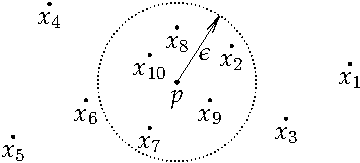
\includegraphics{figures/sequence-convergence-metric}
\caption{Sequence converging to $p$.  The first 10 points 
are shown and $M=7$ for this $\epsilon$.\label{fig:sequence-convergence-metric}}
\end{myfig}
\end{defn}

Let us prove that the limit is unique.  

\begin{prop} \label{prop:mslimisunique}
A convergent sequence in a metric space has a unique limit.
\end{prop}

\begin{proof}
%NOTE: should be word for word the same as 2.1.6
Suppose the sequence $\{ x_n \}$ has limits $x$ and $y$.
Take an arbitrary $\epsilon > 0$.
From the definition find an $n$ such that 
$d(x_n,x) < \nicefrac{\epsilon}{2}$ and
$d(x_n,y) < \nicefrac{\epsilon}{2}$.  Then
\begin{equation*}
d(y,x)
\leq
d(y,x_n) + d(x_n,x)
<
\frac{\epsilon}{2} + \frac{\epsilon}{2} = \epsilon .
\end{equation*}
So $x=y$ and the limit (if it exists) is unique.
\end{proof}

The proofs of the following propositions are left as exercises.

\begin{prop} \label{prop:msconvbound}
A convergent sequence in a metric space is bounded.
\end{prop}

\begin{prop} \label{prop:msconvifa}
A sequence $\{ x_n \}$ in a metric space $(X,d)$ converges to $p \in X$
if and only
if there exists a sequence $\{ a_n \}$ of real numbers such that
\begin{equation*}
d(x_n,p) \leq a_n \quad \text{for all $n \in \N$},
\qquad \text{and} \qquad
\lim_{n\to\infty} a_n = 0.
\end{equation*}
\end{prop}

\begin{prop} \label{prop:mssubseq}
Let $\{ x_n \}$ be a sequence in a metric space $(X,d)$.
\begin{enumerate}[(i)]
\item If $\{ x_n \}$ converges to $p \in X$, then every subsequence $\{ x_{n_k} \}$
converges to $p$.
\item If for some $K \in \N$ the $K$-tail $\{ x_n \}_{n=K+1}^\infty$
converges to $p \in X$, then
 $\{ x_n \}$ converges to $p$.
\end{enumerate}
\end{prop}

\begin{example}
Take $C([0,1],\R)$ be the set of continuous functions with the metric being
the uniform metric.  We saw that we obtain a metric space.
If we look at the definition of convergence, we notice that it is identical
to uniform convergence.  That is, $\{ f_n \}$ converges uniformly if and only
if it converges in the metric space sense.
\end{example}

%\begin{remark}
%It is perhaps surprising that on the set of functions $f \colon [a,b] \to
%\R$ (continuous or not)
%there is no metric that gives pointwise convergence.  Although the proof of
%this fact is beyond the scope of this book.
%\end{remark}

\subsection{Convergence in euclidean space}

In $\R^n$, a sequence converges if and only if every
component converges:

\begin{prop} \label{prop:msconveuc}
Let $\{ x_j \}_{j=1}^\infty$ be a sequence in $\R^n$,
where $x_j = \bigl(x_{j,1},x_{j,2},\ldots,x_{j,n}\bigr) \in \R^n$.
Then $\{ x_j \}_{j=1}^\infty$ converges if and only if
$\{ x_{j,k} \}_{j=1}^\infty$ converges for every $k=1,2,\ldots,n$, in which case
\begin{equation*}
\lim_{j\to\infty}
x_j =
\Bigl(
\lim_{j\to\infty} x_{j,1},
\lim_{j\to\infty} x_{j,2},
\ldots,
\lim_{j\to\infty} x_{j,n}
\Bigr) .
\end{equation*}
\end{prop}

\begin{proof}
Suppose
the sequence
$\{ x_j \}_{j=1}^\infty$ converges to
$y = (y_1,y_2,\ldots,y_n) \in \R^n$.
Given $\epsilon > 0$, there exists an $M$, such that for all
$j \geq M$ we have
\begin{equation*}
d(y,x_j) < \epsilon.
\end{equation*}
Fix some $k=1,2,\ldots,n$.  For $j \geq M$ we have
\begin{equation*}
\bigl\lvert y_k - x_{j,k} \bigr\rvert
=
\sqrt{{\bigl(y_k - x_{j,k} \bigr)}^2}
\leq
\sqrt{\sum_{\ell=1}^n {\bigl(y_\ell-x_{j,\ell}\bigr)}^2}
= d(y,x_j) < \epsilon .
\end{equation*}
Hence the sequence $\{ x_{j,k} \}_{j=1}^\infty$ converges to $y_k$.

For the other direction, suppose 
$\{ x_{j,k} \}_{j=1}^\infty$ converges to $y_k$ for every $k=1,2,\ldots,n$.
Given $\epsilon > 0$, pick an $M$, such that if $j \geq M$ then 
$\bigl\lvert y_k-x_{j,k} \bigr\rvert < \nicefrac{\epsilon}{\sqrt{n}}$ for all
$k=1,2,\ldots,n$.  Then
\begin{equation*}
d(y,x_j)
=
\sqrt{\sum_{k=1}^n {\bigl(y_k-x_{j,k}\bigr)}^2}
<
\sqrt{\sum_{k=1}^n {\left(\frac{\epsilon}{\sqrt{n}}\right)}^2}
=
\sqrt{\sum_{k=1}^n \frac{{\epsilon^2}}{n}}
= \epsilon .
\end{equation*}
That is, the sequence $\{ x_j \}$ converges to
$y = (y_1,y_2,\ldots,y_n) \in \R^n$.
\end{proof}

\begin{example}
The set $\C$ of complex numbers $z = x+iy$ is considered 
as the metric space $\R^2$.  The proposition says that the
sequence $\{ z_j \}_{j=1}^\infty = \{ x_j + iy_j \}_{j=1}^\infty$ converges
to $z = x+iy$
if and only if $\{ x_j \}$ converges to $x$ and 
$\{ y_j \}$ converges to $y$.
\end{example}

\subsection{Convergence and topology}

The topology, that is, the set of open sets of a space encodes which
sequences converge.

\begin{prop} \label{prop:msconvtopo}
Let $(X,d)$ be a metric space and $\{x_n\}$ a sequence in $X$.  Then
$\{ x_n \}$ converges to $x \in X$ if and only if for every open neighborhood
$U$ of $x$, there exists an $M \in \N$ such that for all $n \geq M$
we have $x_n \in U$.
\end{prop}

\begin{proof}
First suppose $\{ x_n \}$ converges.  Let $U$ be an open neighborhood
of $x$, then there exists an $\epsilon > 0$ such that $B(x,\epsilon) \subset
U$.  As the sequence converges, find an $M \in \N$ such that for all $n \geq
M$ we have $d(x,x_n) < \epsilon$ or in other words $x_n \in B(x,\epsilon)
\subset U$.

Let us prove the other direction.  Given $\epsilon > 0$ let $U =
B(x,\epsilon)$ be the neighborhood of $x$.  Then there is an $M \in \N$
such that for $n \geq M$ we have $x_n \in U = B(x,\epsilon)$ or in other
words, $d(x,x_n) < \epsilon$.
\end{proof}

A set is closed when it contains the limits of its convergent sequences.

\begin{prop} \label{prop:msclosedlim}
Let $(X,d)$ be a metric space, $E \subset X$ a closed set,
and $\{ x_n \}$ a sequence in $E$ that converges to some $x \in X$.
Then $x \in E$.
\end{prop}

\begin{proof}
Let us prove the contrapositive.
Suppose $\{ x_n \}$ is a sequence in $X$ that converges to $x \in E^c$.
As $E^c$ is open, \propref{prop:msconvtopo} says that there is
an $M$ such that for all $n \geq M$,
$x_n \in E^c$.  So $\{ x_n \}$  is not a sequence in $E$.
\end{proof}

To take a closure of a set $A$, we take $A$, and we throw in 
points that are limits of sequences in $A$.

\begin{prop} \label{prop:msclosureapprseq}
Let $(X,d)$ be a metric space and $A \subset X$.
Then $x \in \widebar{A}$ if and only if there exists a sequence $\{ x_n \}$ of
elements in $A$ such that $\lim\, x_n = x$.
\end{prop}

\begin{proof}
Let $x \in \widebar{A}$.  For every $n \in \N$,
by
\propref{prop:msclosureappr} there
exists a point $x_n \in B(x,\nicefrac{1}{n}) \cap A$.
As $d(x,x_n) < \nicefrac{1}{n}$, we have $\lim\, x_n = x$.

For the other direction, see \exerciseref{exercise:reverseclosedseq}.
\end{proof}

\subsection{Exercises}

\begin{exbox}
\begin{exercise} \label{exercise:reverseclosedseq}
Finish the proof of 
\propref{prop:msclosureapprseq}.
Let $(X,d)$ be a metric space and
let $A \subset X$.  Let $E$ be the set of all $x \in X$ such that there
exists a sequence $\{ x_n \}$ in $A$ that converges to $x$.  Show 
$E = \widebar{A}$.
\end{exercise}

\begin{exercise}
\begin{exparts}
\item
Show that $d(x,y) = \min \{ 1, \abs{x-y} \}$ defines a metric on $\R$.
\item
Show that a sequence converges in $(\R,d)$ if and only if it converges
in the standard metric.
\item
Find a bounded sequence in $(\R,d)$ that
contains no convergent subsequence.
\end{exparts}
\end{exercise}

\begin{exercise}
Prove \propref{prop:msconvbound}.
\end{exercise}

\begin{exercise}
Prove \propref{prop:msconvifa}.
\end{exercise}

\begin{exercise}
Suppose $\{x_n\}_{n=1}^\infty$ converges to $x$.  Suppose $f \colon \N
\to \N$ is a one-to-one function.  Show that
$\{ x_{f(n)} \}_{n=1}^\infty$ converges to $x$.
\end{exercise}

\begin{exercise}
If $(X,d)$ is a metric space where $d$ is the discrete metric.  Suppose 
$\{ x_n \}$ is a convergent sequence in $X$.  Show that there exists
a $K \in \N$ such that for all $n \geq K$ we have $x_n = x_K$.
\end{exercise}

\begin{exercise}
A set $S \subset X$ is said to be \emph{dense} in $X$ if
$X \subset \widebar{S}$ or in other words if for every $x \in X$,
there exists a sequence $\{ x_n \}$ in $S$ that converges to $x$.  Prove
that $\R^n$ contains a countable dense subset.
\end{exercise}

\begin{exercise}[Tricky]
Suppose $\{ U_n \}_{n=1}^\infty$ be a decreasing ($U_{n+1} \subset U_n$ for
all $n$) sequence of open sets in a metric space $(X,d)$ such that
$\bigcap_{n=1}^\infty U_n = \{ p \}$ for some $p \in X$.  Suppose 
$\{ x_n \}$ is a sequence of points in $X$ such that $x_n \in U_n$.  Does
$\{ x_n \}$ necessarily converge to $p$?  Prove or construct a counterexample.
\end{exercise}

\begin{exercise}
Let $E \subset X$ be closed and
let $\{ x_n \}$ be a sequence in $X$ converging to $p \in X$.  Suppose
$x_n \in E$ for infinitely many $n \in \N$.  Show $p \in E$.
\end{exercise}

\begin{exercise} \label{exercise:extendedrealsmetric}
Take $\R^* = \{ -\infty \} \cup \R \cup \{ \infty \}$ be the extended reals.
Define $d(x,y) = \bigl\lvert \frac{x}{1+\abs{x}} - \frac{y}{1+\abs{y}}
\bigr\rvert$
if $x, y \in \R$,
define $d(\infty,x) = \bigl\lvert 1 - \frac{x}{1+\abs{x}} \bigr\rvert$,
$d(-\infty,x) = \bigl\lvert 1 + \frac{x}{1+\abs{x}} \bigr\rvert$
for all $x \in \R$, and
let $d(\infty,-\infty) = 2$.
\begin{exparts}
\item
Show that $(\R^*,d)$ is a metric space.
\item
Suppose $\{ x_n \}$ is a sequence of real numbers such that
for every $M \in \R$, there exists an $N$ such that
$x_n \geq M$ for all $n \geq N$.  Show that $\lim\, x_n = \infty$ in
$(\R^*,d)$.
\item
Show that a sequence of real numbers converges to a real number
in $(\R^*,d)$ if and
only if it converges in $\R$ with the standard metric.
\end{exparts}
\end{exercise}

\begin{exercise}
Suppose $\{ V_n \}_{n=1}^\infty$ is a collection of open sets
in $(X,d)$
such that $V_{n+1} \supset V_n$.  Let $\{ x_n \}$ be a sequence
such that $x_n \in V_{n+1} \setminus V_n$ and suppose 
$\{ x_n \}$ converges to $p \in X$.  Show that $p \in \partial V$
where $V = \bigcup_{n=1}^\infty V_n$.
\end{exercise}

\begin{exercise}
Prove \propref{prop:mssubseq}.
\end{exercise}

\begin{exercise}
Let $(X,d)$ be a metric space and $\{ x_n \}$ a sequence in $X$.
Prove that $\{ x_n \}$ converges to $p \in X$
if and only if
every subsequence of $\{ x_n \}$ has a subsequence that
converges to $p$.
\end{exercise}

\begin{exercise}
Consider $\R^n$, and let $d$ be the standard euclidean metric.
Let $d'(x,y) = \sum_{\ell=1}^n \abs{x_\ell-y_\ell}$
and $d''(x,y) = \max \{ \abs{x_1-y_1},\abs{x_2-y_2},\cdots,\abs{x_n-y_n}
\}$.
\begin{exparts}
\item
Use \exerciseref{exercise:mscross}, to show that
$(\R^n,d')$ and
$(\R^n,d'')$ are metric spaces.
\item
Let $\{ x_j \}_{j=1}^\infty$ be a sequence in $\R^n$ and $p \in \R^n$.
Prove that the following statements are equivalent:
\begin{exnumparts}
\item
$\{ x_j \}$ converges to $p$ in $(\R^n,d)$.
\item
$\{ x_j \}$ converges to $p$ in $(\R^n,d')$.
\item
$\{ x_j \}$ converges to $p$ in $(\R^n,d'')$.
\end{exnumparts}
\end{exparts}
\end{exercise}
\end{exbox}

%%%%%%%%%%%%%%%%%%%%%%%%%%%%%%%%%%%%%%%%%%%%%%%%%%%%%%%%%%%%%%%%%%%%%%%%%%%%%%

\section{Completeness and compactness}
\label{sec:metcompact}

\subsection{Cauchy sequences and completeness}

Just like with sequences of real numbers we define Cauchy sequences.

\begin{defn}
Let $(X,d)$ be a metric space.
A sequence $\{ x_n \}$ in $X$ is a \emph{\myindex{Cauchy sequence}} if
for every $\epsilon > 0$ there exists an $M \in \N$ such that
for all $n \geq M$ and all $k \geq M$ we have
\begin{equation*}
d(x_n, x_k) < \epsilon .
\end{equation*}
\end{defn}

The definition is again simply a translation of the concept
from the real numbers to metric spaces,
provided we equip the real numbers with
the standard metric $d(x,y) = \abs{x-y}$.

\begin{prop}
A convergent sequence in a metric space is Cauchy.
\end{prop}

\begin{proof}
Suppose $\{ x_n \}$ converges to $x$.
Given $\epsilon > 0$ there is an $M$ such that for $n \geq M$
we have $d(x,x_n) < \nicefrac{\epsilon}{2}$.  Hence
for all $n,k \geq M$ we have
$d(x_n,x_k) \leq d(x_n,x) + d(x,x_k) < \nicefrac{\epsilon}{2} +
\nicefrac{\epsilon}{2} = \epsilon$.
\end{proof}

\begin{defn}
Let $(X,d)$ be a metric space.  We say $X$ is
\emph{\myindex{complete}} or \emph{\myindex{Cauchy-complete}}
if every Cauchy sequence $\{ x_n \}$ in $X$
converges to an $x \in X$.
\end{defn}

\begin{prop}
The space $\R^n$ with the standard metric is a complete metric space.
\end{prop}

We assume the reader has seen the proof of completeness in $\R = \R^1$,
and we reduce the completeness in $\R^n$ to the one dimensional case.

\begin{proof}
Let $\{ x_j \}_{j=1}^\infty$ be a Cauchy sequence
in $\R^n$, where $x_j = \bigl(x_{j,1},x_{j,2},\ldots,x_{j,n}\bigr) \in \R^n$.
Given $\epsilon > 0$, there exists an $M$ such that
$d(x_i,x_j) < \epsilon$
for all
$i,j \geq M$.

Fix some $k=1,2,\ldots,n$, for $i,j \geq M$ we have
\begin{equation*}
\bigl\lvert x_{i,k} - x_{j,k} \bigr\rvert
=
\sqrt{{\bigl(x_{i,k} - x_{j,k}\bigr)}^2}
\leq
\sqrt{\sum_{\ell=1}^n {\bigl(x_{i,\ell}-x_{j,\ell}\bigr)}^2}
= d(x_i,x_j) < \epsilon .
\end{equation*}
Hence the sequence $\{ x_{j,k} \}_{j=1}^\infty$ is Cauchy.  As $\R$ is
complete the sequence converges; there exists an $y_k \in \R$ such that
$y_k = \lim_{j\to\infty} x_{j,k}$.
Write $y = (y_1,y_2,\ldots,y_n) \in \R^n$.
By \propref{prop:msconveuc}, $\{ x_j \}$ converges
to $y \in \R^n$ and hence $\R^n$ is complete.
\end{proof}

A subset of $\R^n$ with the subspace metric need not be
complete.  For example, $(0,1]$ with the subspace metric is not
complete as $\{ \nicefrac{1}{n} \}$ is a Cauchy sequence in $(0,1]$
with no limit in $(0,1]$.  But see also
\exerciseref{exercise:closedcomplete}.

In the language of metric spaces,
as uniform limits of continuous functions are continuous,
the metric space
$C([a,b],\R)$ of \exampleref{example:msC01} is complete.
The proof follows by ``unrolling the definitions,'' 
and is left as an exercise.

\begin{prop} \label{prop:CabRcomplete}
The space of continuous functions $C([a,b],\R)$ with the uniform
norm as metric is a complete metric space.
\end{prop}

Once we have one complete metric space, any closed subspace is
also a complete metric space.  After all, one way
to think of a closed set is that it contains all points
that can be reached from the set via a sequence.
The proof is again an exercise.

\begin{prop} \label{prop:closedcomplete}
Suppose $(X,d)$ is a complete metric space and $E \subset X$
is closed, then $E$ is a complete metric space with the subspace topology.
\end{prop}

\subsection{Compactness}

\begin{defn}
Let $(X,d)$ be a metric space and $K \subset X$. 
The set $K$ is said to be \emph{\myindex{compact}}
if for any collection
of open sets $\{ U_{\lambda} \}_{\lambda \in I}$ such that
\begin{equation*}
K \subset \bigcup_{\lambda \in I} U_\lambda ,
\end{equation*}
there exists a finite subset
$\{ \lambda_1, \lambda_2,\ldots,\lambda_k \} \subset I$
such that
\begin{equation*}
K \subset \bigcup_{j=1}^k U_{\lambda_j} .
\end{equation*}
\end{defn}

A collection of open sets $\{ U_{\lambda} \}_{\lambda \in I}$ as above is
said to be an \emph{\myindex{open cover}} of $K$.  So a way to say that
$K$ is compact is to say that \emph{every open cover of $K$ has a finite
\myindex{subcover}}.

\begin{example}
Let $\R$ be the metric space with the standard metric.

The set $\R$ is not compact.  Proof: Take the sets $U_j = (-j,j)$.
Any $x \in \R$ is in some $U_j$, so we have an open cover.
Suppose we have a finite
subcover $\R \subset U_{j_1} \cup U_{j_2} \cup \cdots \cup U_{j_k}$,
and suppose $j_1 < j_2 < \cdots < j_k$.  Then $\R \subset U_{j_k}$, but that is
a contradiction as $j_k \in \R$ on one hand and $j_k \notin U_{j_k} =
(-j_k,j_k)$ on the
other.

The set $(0,1) \subset \R$ is also not compact.  Proof:  Take the 
sets $U_{j} = (\nicefrac{1}{j},1-\nicefrac{1}{j})$ for $j=3,4,5,\ldots$.
As above $(0,1) = \bigcup_{j=3}^\infty U_j$.  And similarly as above,
if there exists a finite subcover, then there is one $U_j$ such that $(0,1)
\subset U_j$, which again leads to a contradiction.

The set $\{ 0 \} \subset \R$ is compact.  Proof: Given any open cover $\{
U_{\lambda} \}_{\lambda \in I}$, there must exist a $\lambda_0$ such that $0
\in U_{\lambda_0}$ as it is a cover.  But then $U_{\lambda_0}$ gives a
finite subcover.

We will prove below that $[0,1]$, and in fact any closed and bounded
interval $[a,b]$ is compact.
\end{example}

\begin{prop}
Let $(X,d)$ be a metric space.  A compact set $K \subset X$ is closed and
bounded.
\end{prop}

\begin{proof}
First, we prove that a compact set is bounded.
Fix $p \in X$.  We have the open cover
\begin{equation*}
K \subset \bigcup_{n=1}^\infty B(p,n) = X .
\end{equation*}
If $K$ is compact, then there exists some set of indices
$n_1 < n_2 < \ldots < n_k$ such that
\begin{equation*}
K \subset \bigcup_{j=1}^k B(p,n_j) = B(p,n_k) .
\end{equation*}
As $K$ is contained in a ball, $K$ is bounded.
See left hand side of \figureref{fig:compactbndclosed}.

Next, we show a set that is not closed is not compact.  Suppose 
$\widebar{K} \not= K$, that is, there is a point $x \in \widebar{K}
\setminus K$.
If $y \not= x$, then
$y \notin C(x,\nicefrac{1}{n})$
for $n \in \N$
such that $\nicefrac{1}{n} < d(x,y)$.
Furthermore $x \notin K$, so
\begin{equation*}
K \subset \bigcup_{n=1}^\infty {C(x,\nicefrac{1}{n})}^c .
\end{equation*}
A closed ball is closed, so its complement ${C(x,\nicefrac{1}{n})}^c$ is open, and
we have an open cover.
If we take any
finite collection of indices $n_1 < n_2 < \ldots < n_k$, then 
\begin{equation*}
\bigcup_{j=1}^k {C(x,\nicefrac{1}{n_j})}^c 
=
{C(x,\nicefrac{1}{n_k})}^c 
\end{equation*}
As $x$ is in the closure of $K$,
then
$C(x,\nicefrac{1}{n_k}) \cap K \not= \emptyset$.  So there is no
finite subcover and $K$ is not compact.
See right hand side of \figureref{fig:compactbndclosed}.
\end{proof}

\begin{myfig}
\subimport*{figures/}{compactbnd.pdf_t}
\qquad \qquad
\subimport*{figures/}{compactclosed.pdf_t}
\caption{Proving compact set is bounded (left) and closed (right).\label{fig:compactbndclosed}}
\end{myfig}

We prove below that 
in finite dimensional euclidean space
every closed bounded set is compact.
So closed bounded sets
of $\R^n$ are examples of compact sets.
It is not true that in every metric space, closed and bounded is equivalent
to compact.  A simple example is an incomplete metric space such as
$(0,1)$ with the subspace metric from $\R$.
There are many complete and very useful metric spaces
where closed and bounded is not
enough to give compactness: $C([a,b],\R)$ is a complete metric
space, but the closed unit ball $C(0,1)$ is not compact, see
\exerciseref{exercise:msclbounnotcompt}.  However, see also
\exerciseref{exercise:mstotbound}.

A useful property of compact sets in a metric space is that every
sequence in the set has a convergent subsequence converging
to a point in the set.
Such sets are called
\emph{\myindex{sequentially compact}}.
Let us prove that in the
context of metric spaces, a set is compact if and only if it is sequentially
compact.
First we prove a lemma.

\begin{lemma}[Lebesgue covering lemma%
\footnote{Named after the French mathematician
\href{https://en.wikipedia.org/wiki/Henri_Lebesgue}{Henri L\'eon Lebesgue}
(1875--1941).
The number $\delta$ is sometimes called the \myindex{Lebesgue number} of the
cover.}]\label{ms:lebesgue}
\index{Lebesgue covering lemma}
Let $(X,d)$ be a metric space and $K \subset X$.  Suppose 
every sequence in $K$ has a subsequence convergent in $K$.  Given
an open cover $\{ U_\lambda \}_{\lambda \in I}$ of $K$, there exists a
$\delta > 0$ such that for every $x \in K$, there exists a $\lambda \in I$
with $B(x,\delta) \subset U_\lambda$.
\end{lemma}

\begin{proof}
We prove the lemma by contrapositive.
If the conclusion is not true, then
there is
an open cover $\{ U_\lambda \}_{\lambda \in I}$ of $K$ with
the following property.
For every $n \in \N$ there exists an $x_n \in K$ such that
$B(x_n,\nicefrac{1}{n})$ is not a subset of any $U_\lambda$.
Take any $x \in K$.  There is
a $\lambda \in I$ such that $x \in U_\lambda$.  As $U_\lambda$ is open,
there is an $\epsilon > 0$ 
such that $B(x,\epsilon) \subset U_\lambda$.  Take $M$ such that
$\nicefrac{1}{M} < \nicefrac{\epsilon}{2}$.  If $y \in 
B(x,\nicefrac{\epsilon}{2})$ and $n \geq M$, then 
\begin{equation*}
B(y,\nicefrac{1}{n}) \subset
B(y,\nicefrac{1}{M}) \subset
B(y,\nicefrac{\epsilon}{2}) \subset B(x,\epsilon)
\subset U_\lambda ,
\end{equation*}
where 
$B(y,\nicefrac{\epsilon}{2}) \subset B(x,\epsilon)$
follows by triangle inequality.
See \figureref{fig:lebesguedelta}.
In other words, for all $n \geq M$, $x_n \notin B(x,\nicefrac{\epsilon}{2})$. 
The sequence cannot have a subsequence converging to $x$.  As $x \in K$ was
arbitrary we are done.
\end{proof}

\begin{myfig}
\subimport*{figures/}{lebesguedelta.pdf_t}
\caption{Proof of Lebesgue covering lemma.
Note that $B(y,\nicefrac{\epsilon}{2}) \subset
B(x,\epsilon)$ by triangle inequality.\label{fig:lebesguedelta}}
\end{myfig}

It is important to recognize what the lemma says.  It says that
if $K$ is sequentially compact, then given any
cover there is a single $\delta > 0$.  The $\delta$ depends on the cover,
but of course it does not depend on $x$.

For example, let $K = [-10,10]$ and for $n \in \Z$ let $U_n =
(n,n+2)$ define sets in an open cover.
Take $x \in K$. There is an $n \in \Z$, 
such that $n \leq x < n+1$.
If $n \leq x < n+\nicefrac{1}{2}$, then
$B\bigl(x,\nicefrac{1}{2}\bigr) \subset U_{n-1}$.  If
If $n+ \nicefrac{1}{2} \leq x < n+1$, then
$B\bigl(x,\nicefrac{1}{2}\bigr) \subset U_{n}$.  So $\delta =
\nicefrac{1}{2}$.  If instead we let $U'_n =
\bigl(\frac{n}{2},\frac{n+2}{2} \bigr)$, then we again obtain an open
cover, but now the best $\delta$ we can find is $\nicefrac{1}{4}$.

On the other hand, $\N \subset \R$ is not sequentially compact.
It is an exercise to find a cover for which no $\delta > 0$ works.


\begin{thm} \label{thm:mscompactisseqcpt}
Let $(X,d)$ be a metric space.  Then $K \subset X$ is compact if
and only if every sequence in $K$ has a subsequence converging to
a point in $K$.
\end{thm}

\begin{proof}
Claim: \emph{Let $K \subset X$ be a subset of $X$ and
$\{ x_n \}$ a sequence in $K$.  Suppose that for each $x \in K$,
there is a ball $B(x,\alpha_x)$ for some $\alpha_x > 0$ such that
$x_n \in B(x,\alpha_x)$ for only finitely many $n \in \N$.
Then $K$ is not compact.}

Proof of the claim:
Notice
\begin{equation*}
K \subset \bigcup_{x \in K} B(x,\alpha_x) .
\end{equation*}
Any finite collection of these balls is going to contain only finitely many
$x_n$.  Thus for any finite collection of such balls there is an $x_n \in K$
that is not in the union.  Therefore, $K$ is not compact and the claim is
proved.

So suppose that $K$ is compact and $\{ x_n \}$ is a sequence in $K$.
Then there exists an $x \in K$ such that
for any $\delta > 0$,
$B(x,\delta)$ contains $x_k$ for infinitely many $k \in \N$.
We define the subsequence inductively.
The ball $B(x,1)$ contains some $x_k$ so let $n_1 = k$.
Suppose $n_{j-1}$ is defined.
There must exist a $k > n_{j-1}$
such that $x_k \in B(x,\nicefrac{1}{j})$.  So define
$n_j = k$.
We now posses a subsequence $\{ x_{n_j} \}_{j=1}^\infty$.
Since
$d(x,x_{n_j}) < \nicefrac{1}{j}$,  \propref{prop:msconvifa} says
$\lim\, x_{n_j} = x$.

For the other direction, suppose every sequence in $K$
has a 
subsequence converging in $K$.
Take
an open cover $\{ U_\lambda \}_{\lambda \in I}$ of $K$.
Using the Lebesgue covering lemma above, find a $\delta > 0$
such that for every $x \in K$, there is a $\lambda \in I$ with
$B(x,\delta) \subset U_\lambda$.

Pick $x_1 \in K$ and find $\lambda_1 \in I$ such that $B(x_1,\delta) \subset
U_{\lambda_1}$.
If $K \subset U_{\lambda_1}$, we stop as we have found a
finite subcover.
Otherwise, there must be
a point $x_2 \in K \setminus U_{\lambda_1}$.
Note that $d(x_2,x_1) \geq \delta$.
There must exist some $\lambda_2 \in I$ such that
$B(x_2,\delta) \subset U_{\lambda_2}$.
We work inductively.  Suppose $\lambda_{n-1}$ is defined.
Either
$U_{\lambda_1} \cup
U_{\lambda_2} \cup \cdots \cup
U_{\lambda_{n-1}}$ is a finite cover of $K$, in which case we
stop, or
there must be 
a point $x_n \in K \setminus \bigl( U_{\lambda_1} \cup
U_{\lambda_2} \cup \cdots \cup
U_{\lambda_{n-1}}\bigr)$.
Note that $d(x_n,x_j) \geq \delta$ for all $j = 1,2,\ldots,n-1$.
Next, there must be some $\lambda_n \in I$
such that $B(x_n,\delta) \subset U_{\lambda_n}$.
See \figureref{fig:seqcompactiscompact}.

\begin{myfig}
\subimport*{figures/}{seqcompactiscompact.pdf_t}
\caption{Covering $K$ by $U_{\lambda}$.  The points
$x_1,x_2,x_3,x_4$, 
the three sets 
$U_{\lambda_1}$,
$U_{\lambda_2}$,
$U_{\lambda_2}$,
and 
the first three balls
of radius $\delta$ are drawn.\label{fig:seqcompactiscompact}}
\end{myfig}

Either at some point we obtain a finite subcover of $K$,
or we obtain an
infinite
sequence $\{ x_n \}$ as above.
For contradiction, suppose that
there is no finite subcover and we have the sequence $\{ x_n \}$.
For all $n$ and $k$, $n \not= k$, 
we have $d(x_n,x_k) \geq \delta$,
so no subsequence of $\{ x_n \}$ can be
Cauchy.  Hence no subsequence of $\{ x_n \}$ can be convergent,
which is a contradiction.
\end{proof}

\begin{example}
The Bolzano--Weierstrass Theorem for sequences of real numbers
says that any bounded sequence in $\R$ has a convergent
subsequence.  Therefore, any sequence in a closed interval $[a,b] \subset \R$ has 
a convergent subsequence.  The limit must also be in $[a,b]$ as limits
preserve non-strict inequalities.  Hence a closed bounded interval $[a,b]
\subset \R$ is compact.
\end{example}

\begin{prop}
Let $(X,d)$ be a metric space and let $K \subset X$ be compact.  If
$E \subset K$ is a closed set, then $E$ is compact.
\end{prop}

Because $K$ is closed then $E$ is closed in $K$ if
and only if it is closed in $X$,
see \propref{prop:topology:subspacesame}.

\begin{proof}
Let $\{ x_n \}$ be a sequence in $E$.  It is also a sequence in $K$.
Therefore, it has a convergent subsequence $\{ x_{n_j} \}$ that converges to
some $x \in K$.  As $E$ is closed the limit of a sequence in $E$ is also in $E$
and so $x \in E$.  Thus $E$ must be compact.
\end{proof}

\begin{thm}[Heine--Borel%
\footnote{Named after the German mathematician 
\href{https://en.wikipedia.org/wiki/Eduard_Heine}{Heinrich Eduard Heine}
(1821--1881),
and the French mathematician
\href{https://en.wikipedia.org/wiki/\%C3\%89mile_Borel}{F\'elix \'Edouard Justin \'Emile Borel}
(1871--1956).}]%
\index{Heine--Borel Theorem}
\label{thm:msbw}
A closed bounded subset $K \subset \R^n$ is compact.
\end{thm}

So subsets of $\R^n$ are compact if and only if they are closed and bounded,
a condition that is much easier to check.
Let us reiterate that the Heine--Borel Theorem only holds for $\R^n$ and not
for metric spaces in general.  In general, compact implies closed and
bounded, but not vice-versa.

\begin{proof}
For $\R = \R^1$ if $K \subset \R$ is closed and bounded, then
any sequence $\{ x_k \}$ in $K$ is bounded, so it has a convergent
subsequence by
the Bolzano--Weierstrass Theorem.
As $K$ is closed, the limit of the subsequence must be an element of
$K$.  So $K$ is compact.

Let us carry out the proof for $n=2$ and leave arbitrary $n$ as an exercise.
As $K \subset \R^2$ is bounded, there exists a set
$B=[a,b]\times[c,d] \subset \R^2$ such that $K \subset B$.  We will show
that $B$ is compact.  Then $K$, being a closed subset of a compact $B$, is
also compact.  

Let $\bigl\{ (x_k,y_k) \bigr\}_{k=1}^\infty$ be a sequence in $B$.  That is,
$a \leq x_k \leq b$ and
$c \leq y_k \leq d$ for all $k$.  A bounded sequence of real numbers
has a convergent
subsequence so there is a subsequence $\{ x_{k_j} \}_{j=1}^\infty$
that is convergent.  The subsequence 
$\{ y_{k_j} \}_{j=1}^\infty$ is also a bounded sequence so there exists
a subsequence
$\{ y_{k_{j_i}} \}_{i=1}^\infty$ that is convergent.  A subsequence of a
convergent sequence is still convergent, so 
$\{ x_{k_{j_i}} \}_{i=1}^\infty$ is convergent.
Let
\begin{equation*}
x = \lim_{i\to\infty} x_{k_{j_i}}
\qquad \text{and} \qquad
y = \lim_{i\to\infty} y_{k_{j_i}} .
\end{equation*}
By \propref{prop:msconveuc},
$\bigl\{ (x_{k_{j_i}},y_{k_{j_i}}) \bigr\}_{i=1}^\infty$ converges to $(x,y)$.
Furthermore, as $a \leq x_k \leq b$ and
$c \leq y_k \leq d$ for all $k$, we know that $(x,y) \in B$.
\end{proof}

\begin{prop}
Suppose $(X,d)$ is a complete metric space
and suppose we have a countably infinite
collection of nonempty compact sets $E_1 \supset E_2 \supset E_3 \supset
\cdots$.  Then
\begin{equation*}
\bigcap_{j=1}^\infty E_j \not= \emptyset .
\end{equation*}
\end{prop}

The proof is left as an exercise below.

\begin{example}
The discrete metric provides interesting counterexamples again.
Let $(X,d)$ be a metric space with the discrete metric, that is $d(x,y) = 1$
if $x \not= y$.  Suppose
$X$ is an infinite set.  Then:
\begin{enumerate}[(i)]
\item $(X,d)$ is a complete metric space.
\item Any subset $K \subset X$ is closed and bounded.
\item A subset $K \subset X$ is compact if and only if it is a finite set.
\item The conclusion of the Lebesgue covering lemma is always satisfied with
e.g. $\delta = \nicefrac{1}{2}$, even for noncompact $K \subset X$.
\end{enumerate}
The proofs
of the statements above are either trivial or are relegated to the exercises
below.
\end{example}

\begin{remark}
A subtle issue with Cauchy sequences, completeness, compactness,
and convergence is that compactness and convergence only depend on the
topology, that is, on which sets are the open sets.  On the other hand,
Cauchy sequences and completeness depend on the actual metric.
See \exerciseref{exercise:cauchydepndsonmetric}.
\end{remark}

\subsection{Exercises}

\begin{exbox}
\begin{exercise}
Let $(X,d)$ be a metric space and $A$ a finite subset of $X$.
Show that $A$ is compact.
\end{exercise}

\begin{samepage}
\begin{exercise}
Let $A = \{ \nicefrac{1}{n} : n \in \N \} \subset \R$.
\begin{exparts}
\item
Show that $A$ is
not compact directly using the definition.
\item
Show that $A \cup \{ 0 \}$ is
compact directly using the definition.
\end{exparts}
\end{exercise}
\end{samepage}


\begin{exercise}
Let $(X,d)$ be a metric space with the discrete metric.
\begin{exparts}
\item
Prove that $X$ is complete.
\item
Prove that $X$ is compact if and only if $X$ is a finite set.
\end{exparts}
\end{exercise}

\begin{exercise}
\begin{exparts}
\item
Show that the union of finitely many compact sets is a compact set.
\item
Find an example where the union of infinitely many compact sets is not
compact.
\end{exparts}
\end{exercise}

\begin{exercise}
Prove \thmref{thm:msbw} for arbitrary dimension.
Hint: The trick is to use the correct notation.
\end{exercise}

\begin{exercise}
Show that a compact set $K$ is a complete metric space (using the subspace
metric).
\end{exercise}

\begin{exercise} \label{exercise:CabRcomplete}
Let $C([a,b],\R)$ be the metric space as in \exampleref{example:msC01}.  Show that
$C([a,b],\R)$ is a complete metric space.
\end{exercise}

\begin{exercise}[Challenging] \label{exercise:msclbounnotcompt}
Let $C([0,1],\R)$ be the metric space of \exampleref{example:msC01}.  Let $0$
denote the zero function.  Then show that the closed ball
$C(0,1)$ is not compact (even though it is closed and bounded).
Hints: Construct a sequence of distinct continuous functions $\{ f_n \}$ such that
$d(f_n,0) = 1$ and $d(f_n,f_k) = 1$ for all $n \not= k$.  Show that
the set $\{ f_n : n \in \N \} \subset C(0,1)$ is closed but not compact.
\end{exercise}

\begin{exercise}[Challenging]
Show that there exists a metric on $\R$ that makes $\R$ into a compact set.
\end{exercise}

\begin{exercise}
Suppose $(X,d)$ is complete and suppose we have a countably infinite
collection of nonempty compact sets $E_1 \supset E_2 \supset E_3 \supset
\cdots$.  Prove $\bigcap_{j=1}^\infty E_j \not= \emptyset$.
\end{exercise}

\begin{exercise}[Challenging]
Let $C([0,1],\R)$ be the metric space of \exampleref{example:msC01}.
Let $K$ be the set of $f \in C([0,1],\R)$ such that
$f$ is equal to a quadratic polynomial, i.e.\ $f(x) = a+bx+cx^2$, and such that
$\abs{f(x)} \leq 1$ for all $x \in [0,1]$,
that is $f \in C(0,1)$.  Show that $K$ is compact.
\end{exercise}

\begin{exercise}[Challenging] \label{exercise:mstotbound}
Let $(X,d)$ be a complete metric space.
Show that $K \subset X$ is compact if and only if $K$ is closed
and such that for every $\epsilon > 0$
there exists a finite set of points $x_1,x_2,\ldots,x_n$ with
$K \subset \bigcup_{j=1}^n B(x_j,\epsilon)$.
Note: Such a set $K$ is said to be \emph{\myindex{totally bounded}},
so in a complete metric space a set is compact if and only
if it is closed and totally bounded.
\end{exercise}

\begin{exercise}
Take $\N \subset \R$ using the standard metric.  Find an open cover of $\N$
such that the conclusion of the Lebesgue covering lemma does not hold.
\end{exercise}

\begin{exercise}
Prove the general \myindex{Bolzano--Weierstrass Theorem}:
Any bounded sequence $\{ x_k
\}$ in $\R^n$ has a convergent subsequence.
\end{exercise}

\begin{exercise}
Let $X$ be a metric space and
$C \subset \sP(X)$ the set of nonempty compact subsets of $X$.
Using the Hausdorff metric from \exerciseref{exercise:mshausdorffpseudo},
show that $(C,d_H)$ is a metric space.  That is, show that
if $L$ and $K$ are nonempty compact subsets then $d_H(L,K) = 0$
if and only if $L=K$.
\end{exercise}

\begin{exercise} \label{exercise:closedcomplete}
Prove \propref{prop:closedcomplete}.  That is,
let $(X,d)$ be a complete metric space and $E \subset X$ a closed set.
Show that $E$ with the subspace metric is a complete metric space.
\end{exercise}

\begin{exercise}
Let $(X,d)$ be an incomplete metric space.  Show that there exists a
closed and bounded set $E \subset X$ that is not compact.
\end{exercise}

\begin{exercise}
Let $(X,d)$ be a metric space and $K \subset X$.
Prove that $K$ is compact as a subset of $(X,d)$ if and only if $K$ is
compact as a subset of itself with the subspace metric.
\end{exercise}

\begin{samepage}
\begin{exercise} \label{exercise:cauchydepndsonmetric}
Consider two metrics on $\R$.
Let $d(x,y) = \abs{x-y}$ be the standard metric,
and let
$d'(x,y) = \bigl\lvert \frac{x}{1+\abs{x}} - \frac{y}{1+\abs{y}}
\bigr\rvert$.
\begin{exparts}
\item
Show that $(\R,d')$ is a metric space (if you have done
\exerciseref{exercise:extendedrealsmetric} the computation is the same).
\item
Show that the topology is the same, that is, a set is open in
$(\R,d)$ if and only if it is open in $(\R,d')$.
\item
Show that a set is compact in
$(\R,d)$ if and only if it is compact in $(\R,d')$.
\item
Show that a sequence converges in $(\R,d)$ if and only if
it converges in $(\R,d')$.
\item
Find a sequence of real numbers that is Cauchy
in $(\R,d')$ but not Cauchy in $(\R,d)$.
\item
While $(\R,d)$ is complete, show that $(\R,d')$ is not complete.
\end{exparts}
\end{exercise}
\end{samepage}

\begin{exercise} \label{exercise:relativelycompactseq}
Let $(X,d)$ be a complete metric space.
We say a set $S \subset X$ is \emph{\myindex{relatively compact}}
if the closure $\widebar{S}$ is compact.
Prove that $S \subset X$ is relatively compact if and only if
given any sequence $\{ x_n \}$ in $S$, there exists a subsequence
$\{ x_{n_k} \}$ that converges (in $X$).
\end{exercise}
\end{exbox}

%%%%%%%%%%%%%%%%%%%%%%%%%%%%%%%%%%%%%%%%%%%%%%%%%%%%%%%%%%%%%%%%%%%%%%%%%%%%%%

\section{Continuous functions}
\label{sec:metcont}

\subsection{Continuity}

\begin{defn}
Let $(X,d_X)$ and $(Y,d_Y)$ be metric spaces and $c \in X$.
Then $f \colon X \to Y$ is
\emph{continuous at $c$}\index{continuous at $c$}
if for every $\epsilon > 0$
there is a $\delta > 0$ such that whenever $x \in X$ and $d_X(x,c) <
\delta$, then
$d_Y\bigl(f(x),f(c)\bigr) < \epsilon$.

\medskip

When $f \colon X \to Y$ is continuous at all $c \in X$, then we simply say
that $f$ is a \emph{continuous function}\index{continuous function!in a
metric space}\index{function!continuous}.
\end{defn}

\begin{prop} \label{prop:contiscont}
Let $(X,d_X)$ and $(Y,d_Y)$ be metric spaces.
Then $f \colon X \to Y$ is
continuous at $c \in X$
if and only if for every sequence $\{ x_n \}$ in $X$
converging to $c$, the sequence $\{ f(x_n) \}$ converges
to $f(c)$.
\end{prop}

\begin{proof}
Suppose $f$ is continuous at $c$.  Let $\{ x_n \}$ be a
sequence in $X$ converging to $c$.  Given $\epsilon > 0$,
there is a $\delta > 0$ such that $d_X(x,c) < \delta$ implies
$d_Y\bigl(f(x),f(c)\bigr) < \epsilon$.  So take $M$ such that
for all $n \geq M$, we have $d_X(x_n,c) < \delta$, then
$d_Y\bigl(f(x_n),f(c)\bigr) < \epsilon$.  Hence $\{ f(x_n) \}$
converges to $f(c)$.

Now suppose $f$ is not continuous at $c$.
Then there exists an $\epsilon > 0$,
such that for every $n \in \N$ there is an $x_n \in X$,
with
$d_X(x_n,c) < \nicefrac{1}{n}$ such that $d_Y\bigl(f(x_n),f(c)\bigr) \geq
\epsilon$.  So $\{ x_n \}$ converges to $c$, but $\{ f(x_n) \}$
does not converge to $f(c)$.
\end{proof}

\begin{example}
Suppose $f \colon \R^2 \to \R$ is a polynomial.  That is,
\begin{equation*}
\begin{split}
f(x,y) & =
\sum_{j=0}^d
\sum_{k=0}^{d-j}
a_{jk}\,x^jy^k \\
& =
a_{0\,0} + a_{1\,0} \, x +
a_{0\,1} \, y+  
a_{2\,0} \, x^2+  
a_{1\,1} \, xy+  
a_{0\,2} \, y^2+ \cdots +
a_{0\,d} \, y^d ,
\end{split}
\end{equation*}
for some $d \in \N$ (the degree) and $a_{jk} \in \R$.  Then we claim 
$f$ is continuous.  Let $\{ (x_n,y_n) \}_{n=1}^\infty$ be a sequence
in $\R^2$ that converges to $(x,y) \in \R^2$.  We proved that this
means $\lim\, x_n = x$ and $\lim\, y_n = y$.  Then
\begin{equation*}
\lim_{n\to\infty}
f(x_n,y_n) =
\lim_{n\to\infty}
\sum_{j=0}^d
\sum_{k=0}^{d-j}
a_{jk} \, x_n^jy_n^k 
=
\sum_{j=0}^d
\sum_{k=0}^{d-j}
a_{jk} \, x^jy^k
=
f(x,y) .
\end{equation*}
So $f$ is continuous at $(x,y)$, and as $(x,y)$ was arbitrary $f$ is
continuous everywhere.  Similarly, a
polynomial in $n$ variables is continuous.
\end{example}

Be careful about taking limits separately.  In \exerciseref{exercise:dicontR2}
you are asked to prove that the function defined by $f(x,y) = \frac{xy}{x^2+y^2}$
outside the origin and $f(0,0) = 0$, is not continuous at the origin.  See
\figureref{fig:xyxsqysq}.
However, for any $y$, the function $g(x) = f(x,y)$ is
continuous,
and for any $x$, the function $h(y) = f(x,y)$ is continuous.
\begin{myfig}
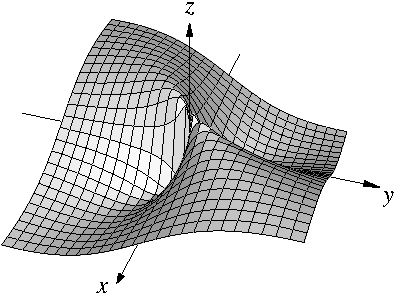
\includegraphics{figures/xyxsqysq}
\caption{Graph of $\frac{xy}{x^2+y^2}$.\label{fig:xyxsqysq}}
\end{myfig}

\begin{example}
Let $X$ be a metric space and $f \colon X \to \C$ a complex-valued
function.  Write $f(p) = g(p) + i h(p)$, where $g \colon X \to \R$
and $h \colon X \to \R$ are the real and imaginary parts of $f$.
Then $f$ is continuous at $c \in X$ if and only if its real
and imaginary parts are continuous at $c$.  
This fact follows because $\{ f(p_n) = g(p_n) + i h(p_n) \}_{n=1}^\infty$
converges to $f(p) = g(p) + i h(p)$ if and only if
$\{ g(p_n) \}$ converges to $g(p)$ and
$\{ h(p_n) \}$ converges to $h(p)$.
\end{example}

\subsection{Compactness and continuity}

Continuous maps do not map closed sets to closed sets.  For example,
$f \colon (0,1) \to \R$ defined by $f(x) = x$ takes the set $(0,1)$, which
is closed in $(0,1)$, to the set $(0,1)$, which is not closed in $\R$.
On the other hand continuous maps do preserve compact sets.

\begin{lemma} \label{lemma:continuouscompact}
Let $(X,d_X)$ and $(Y,d_Y)$ be metric spaces
and $f \colon X \to Y$ a continuous function.  If
$K \subset X$ is a compact set, then $f(K)$ is a compact set.
\end{lemma}

\begin{proof}
A sequence in $f(K)$ can be written as
$\{ f(x_n) \}_{n=1}^\infty$, where
$\{ x_n \}_{n=1}^\infty$ is a sequence in $K$.  The set $K$ is compact and
therefore there is a subsequence
$\{ x_{n_j} \}_{j=1}^\infty$ that converges to some $x \in K$.
By continuity,
\begin{equation*}
\lim_{j\to\infty} f(x_{n_j}) = f(x) \in f(K) .
\end{equation*}
So every sequence in $f(K)$ has a subsequence convergent to 
a point in $f(K)$, and $f(K)$ is compact by \thmref{thm:mscompactisseqcpt}.
\end{proof}

As before, $f \colon X \to \R$ achieves an
\emph{\myindex{absolute minimum}} at $c \in X$ if
\begin{equation*}
f(x) \geq f(c) \qquad \text{ for all $x \in X$.}
\end{equation*}
On the other hand, $f$ achieves an 
\emph{\myindex{absolute maximum}} at $c \in X$ if
\begin{equation*}
f(x) \leq f(c) \qquad \text{ for all $x \in X$.}
\end{equation*}

\begin{thm}
Let $(X,d)$ be a compact metric space
and $f \colon X \to \R$ a continuous function.  Then
$f$ achieves an absolute minimum and maximum on $X$.
In particular, $f$ is bounded.
\end{thm}

\begin{proof}
As $X$ is compact and $f$ is continuous, then
$f(X) \subset \R$ is compact.  Hence $f(X)$ is closed
and bounded.  In particular,
$\sup f(X) \in f(X)$ and
$\inf f(X) \in f(X)$, because both the sup and the inf
can be achieved by sequences in $f(X)$ and $f(X)$ is closed.
Therefore, there is some $x \in X$ such that $f(x) = \sup f(X)$
and some $y \in X$ such that $f(y) = \inf f(X)$.
\end{proof}

\subsection{Continuity and topology}

Let us see how to define continuity in terms of the topology, that is,
the open sets.  We have already seen that topology determines which 
sequences converge, and so it is no wonder that the topology also
determines continuity of functions.

\begin{lemma} \label{lemma:mstopocontloc}
Let $(X,d_X)$ and $(Y,d_Y)$ be metric spaces.
A function $f \colon X \to Y$ is continuous at $c \in X$
if and only if for every open neighborhood $U$ of $f(c)$ in $Y$, the set
$f^{-1}(U)$ contains an open neighborhood of $c$ in $X$.
See \figureref{fig:mscontfuncpt}.
\end{lemma}

\begin{myfig}
\subimport*{figures/}{mscontfuncpt.pdf_t}
\caption{For every neighborhood $U$ of $f(c)$, the set $f^{-1}(U)$ contains an open
neighborhood $W$ of $c$.\label{fig:mscontfuncpt}}
\end{myfig}

\begin{proof}
First suppose that $f$ is continuous at $c$.
Let $U$ be an open neighborhood of $f(c)$
in $Y$, then $B_Y\bigl(f(c),\epsilon\bigr) \subset U$ for some $\epsilon >
0$.  By continuity of $f$, there exists a $\delta > 0$
such that whenever $x$ is such that $d_X(x,c) < \delta$, then
$d_Y\bigl(f(x),f(c)\bigr) < \epsilon$.  In other words,
\begin{equation*}
B_X(c,\delta) \subset f^{-1}\bigl(B_Y\bigl(f(c),\epsilon\bigr)\bigr) \subset
f^{-1}(U) ,
\end{equation*}
and $B_X(c,\delta)$ is an open neighborhood of $c$.

For the other direction,
let $\epsilon > 0$ be given.  If
$f^{-1}\bigl(B_Y\bigl(f(c),\epsilon\bigr)\bigr)$ contains an open
neighborhood $W$ of $c$, it contains a ball.  That is, there is some $\delta > 0$
such that
\begin{equation*}
B_X(c,\delta) \subset W \subset f^{-1}\bigl(B_Y\bigl(f(c),\epsilon\bigr)\bigr) .
\end{equation*}
That means precisely that if $d_X(x,c) < \delta$ then $d_Y\bigl(f(x),f(c)\bigr)
< \epsilon$, and so $f$ is continuous at $c$.
\end{proof}

\begin{thm} \label{thm:mstopocont}
Let $(X,d_X)$ and $(Y,d_Y)$ be metric spaces.  A function $f \colon X \to Y$
is continuous if and only if
for every open $U \subset Y$, $f^{-1}(U)$ is open in $X$.
\end{thm}

The proof follows from \lemmaref{lemma:mstopocontloc} and is left as
an exercise.

\begin{example}
Let $f \colon X \to Y$ be a continuous function.
\thmref{thm:mstopocont} tells us that if $E \subset Y$ is closed, then 
$f^{-1}(E) = X \setminus f^{-1}(E^c)$ is also closed.  Therefore, if
we have a continuous
function $f \colon X \to \R$, then the
\emph{\myindex{zero set}} of $f$, that is, 
$f^{-1}(0) = \{ x \in X :
f(x) = 0 \}$, is closed.

Similarly the set where $f$ is nonnegative, that is,
$f^{-1}\bigl( [0,\infty) \bigr) = \{ x \in X :
f(x) \geq 0 \}$ is closed.  On the other hand the
set where $f$ is positive,
$f^{-1}\bigl( (0,\infty) \bigr) = \{ x \in X :
f(x) > 0 \}$ is open.  
\end{example}

\subsection{Uniform continuity}

As for continuous
functions on the real line, in the definition of continuity
it is sometimes convenient to be able to pick
one $\delta$ for all points.

\begin{defn}
Let $(X,d_X)$ and $(Y,d_Y)$ be metric spaces.
Then $f \colon X \to Y$ is
\emph{uniformly continuous}\index{uniformly continuous!in a metric space}
if for every $\epsilon > 0$
there is a $\delta > 0$ such that whenever $p,q \in X$ and $d_X(p,q) <
\delta$, then
$d_Y\bigl(f(p),f(q)\bigr) < \epsilon$.
\end{defn}

A uniformly continuous function is continuous, but not necessarily
vice-versa as we have seen.

\begin{thm} \label{thm:Xcompactfunifcont}
Let $(X,d_X)$ and $(Y,d_Y)$ be metric spaces.
Suppose $f \colon X \to Y$ is continuous and $X$ is compact.  Then
$f$ is uniformly continuous.
\end{thm}

\begin{proof}
Let $\epsilon > 0$ be given.  For each $c \in X$, pick $\delta_c > 0$ such that
$d_Y\bigl(f(x),f(c)\bigr) < \nicefrac{\epsilon}{2}$
whenever
$x \in B(c,\delta_c)$.
%$d_X(x,c) < \delta_c$.
The balls
$B(c,\delta_c)$ cover $X$, and the space $X$ is compact.  
Apply the \hyperref[ms:lebesgue]{Lebesgue covering lemma} to obtain a 
$\delta > 0$ such that for every $x \in X$, there is a $c \in X$
for which $B(x,\delta) \subset B(c,\delta_c)$.

If $p, q \in X$ where $d_X(p,q) < \delta$,
find a $c \in X$ such that $B(p,\delta) \subset B(c,\delta_c)$.
Then $q \in B(c,\delta_c)$.  By the triangle inequality
and the definition of $\delta_c$ we have
\begin{equation*}
d_Y\bigl(f(p),f(q)\bigr)
\leq
d_Y\bigl(f(p),f(c)\bigr)
+
d_Y\bigl(f(c),f(q)\bigr)
<
\nicefrac{\epsilon}{2}+
\nicefrac{\epsilon}{2} = \epsilon .  \qedhere
\end{equation*}
\end{proof}


\begin{example}
Useful examples of uniformly continuous functions are the so-called
\emph{Lipschitz continuous}%
\index{Lipschitz continuous!in a metric space}%
\index{function!Lipschitz}
functions.  That is, if
$(X,d_X)$ and $(Y,d_Y)$ are metric spaces, then $f \colon X \to Y$
is called Lipschitz or $K$-Lipschitz if there exists a $K \in \R$ such that
\begin{equation*}
d_Y\bigl(f(p),f(q)\bigr) \leq K d_X(p,q)
\ \ \ \ \text{for all } p,q \in X.
\end{equation*}
A Lipschitz function is uniformly continuous:
Take $\delta = \nicefrac{\epsilon}{K}$.
A function can be uniformly continuous
but not Lipschitz,
as we already saw: $\sqrt{x}$ on $[0,1]$
is uniformly continuous but not Lipschitz.

It is worth mentioning that,
if a function is Lipschitz, it tends to be
easiest to simply show it is Lipschitz even if we are only
interested in knowing continuity.
\end{example}

\subsection{Cluster points and limits of functions}

While we haven't started the discussion of continuity with them and we won't
need them until volume II, let us also
translate the idea of a limit of a function from the real line to metric
spaces.
Again we need to start with cluster points.

\begin{defn}
Let $(X,d)$ be a metric space and
$S \subset X$. A point $p \in X$ is called
a \emph{cluster point}\index{cluster point!in a metric space} of $S$
if for every $\epsilon > 0$, the set $B(p,\epsilon) \cap S
\setminus \{ p \}$ is not empty.
\end{defn}

It is not enough that $p$ is in the closure of $S$,
it must be in the closure of
$S \setminus \{ p \}$ (exercise).
So, $p$ is a cluster point if and only if there exists a sequence in $S \setminus
\{ p \}$ that converges to $p$.

\begin{defn}
\index{limit!of a function in a metric space}%
Let $(X,d_X)$, $(Y,d_Y)$ be metric spaces, $S \subset X$, $p \in X$ a cluster point of $S$,
and $f \colon S \to Y$ a function.
Suppose there exists an $L \in Y$ and for every $\epsilon > 0$,
there exists a $\delta > 0$ such that whenever $x \in S \setminus \{ p \}$
and $d_X(x,p) < \delta$, then
\begin{equation*}
d_Y\bigl(f(x),L\bigr) < \epsilon .
\end{equation*}
Then we say $f(x)$
\emph{converges}\index{converges!function in a metric space} to $L$ as $x$ goes
to $p$, and $L$ is the \emph{limit} of $f(x)$ as $x$
goes to $p$.  We write
\glsadd{not:limfunc}
\begin{equation*}
\lim_{x \to p} f(x) \overset{\text{def}}{=} L .
\end{equation*}
Otherwise we say $f$
\emph{diverges}\index{diverges!function in a metric space} at $p$.
\end{defn}

We again used the definite article without showing that the
limit is unique.  We leave the proof of uniqueness as an exercise.

\begin{prop} \label{prop:mslimitisunique}
Let $(X,d_X)$ and $(Y,d_Y)$ be metric spaces, $S \subset X$, $p \in X$
a cluster point of $S$, and let $f \colon S \to Y$ be a function
such that $f(x)$ converges as $x$ goes to $p$.  Then
the limit of $f(x)$ as $x$ goes to $p$ is unique.
\end{prop}

In any metric space, just like in $\R$, continuous limits may be
replaced by sequential limits.  We leave the proof as an
exercise.  The upshot is that we really only need to prove things for
sequential limits.

\begin{lemma}\label{ms:seqflimit:lemma}
Let $(X,d_X)$ and $(Y,d_Y)$ be metric spaces, $S \subset X$, $p \in X$
a cluster point of $S$, and let $f \colon S \to Y$ be a function.

Then
$f(x)$ converges to $L \in Y$ as $x$ goes to $p$ if and only if for every sequence $\{ x_n \}$
in $S \setminus \{p\}$
such that $\lim\, x_n = p$,
the sequence $\{ f(x_n) \}$ converges to $L$.
\end{lemma}

By applying \propref{prop:contiscont} or the definition directly we find
(exercise) that for cluster points $p$ of $S
\subset X$, the function
$f \colon S \to Y$ is continuous at $p$ if and only if
\begin{equation*}
\lim_{x \to p} f(x) = f(p) .
\end{equation*}

\subsection{Exercises}

\begin{exbox}
\begin{exercise}
Consider $\N \subset \R$ with the standard metric.  Let $(X,d)$ be a
metric space and $f \colon X \to \N$ a continuous function.
\begin{exparts}
\item
Prove that if $X$ is connected,
then $f$ is constant (the range of $f$ is a single value).
\item
Find an example where $X$ is disconnected and $f$ is not constant.
\end{exparts}
\end{exercise}

\begin{exercise} \label{exercise:dicontR2}
Let $f \colon \R^2 \to \R$ be defined by $f(0,0) = 0$, and
$f(x,y) = \frac{xy}{x^2+y^2}$ if $(x,y) \not= (0,0)$.
\begin{exparts}
\item
Show that for any fixed $x$,
the function that takes $y$ to $f(x,y)$ is continuous.  Similarly
for any fixed $y$, the function that takes $x$ to $f(x,y)$ is continuous.
\item
Show that $f$ is not continuous.
\end{exparts}
\end{exercise}

\begin{samepage}
\begin{exercise} 
Suppose $(X,d_X)$, $(Y,d_Y)$ be metric spaces and
$f \colon X \to Y$ is continuous.
Let $A \subset X$.
\begin{exparts}
\item
Show that $f(\widebar{A}) \subset \overline{f(A)}$.
\item
Show that the subset can be proper.
\end{exparts}
\end{exercise}
\end{samepage}

\begin{exercise}
Prove \thmref{thm:mstopocont}.  Hint: Use \lemmaref{lemma:mstopocontloc}.
\end{exercise}

\begin{exercise} \label{exercise:msconnconn}
Suppose $f \colon X \to Y$ is continuous for metric spaces $(X,d_X)$
and $(Y,d_Y)$.  Show that if $X$ is connected, then $f(X)$ is connected.
\end{exercise}

\begin{exercise}
Prove the following version of the
Intermediate Value Theorem.  Let $(X,d)$ be a connected
metric space and $f \colon X \to \R$ a continuous function.  Suppose that
there exist $x_0,x_1 \in X$ and $y \in \R$ such that $f(x_0) < y < f(x_1)$.
Then prove that there exists a $z \in X$ such that $f(z) = y$.
Hint: See \exerciseref{exercise:msconnconn}.
\end{exercise}

\begin{exercise}
A continuous function $f \colon X \to Y$ for metric spaces $(X,d_X)$ and
$(Y,d_Y)$ is said to be \emph{\myindex{proper}}
if for every compact set $K \subset Y$, the set $f^{-1}(K)$ is compact.
Suppose a continuous $f \colon (0,1) \to (0,1)$ is proper and $\{ x_n
\}$ is a sequence in $(0,1)$ that converges to $0$.  Show that
$\{ f(x_n) \}$ has no subsequence that converges in $(0,1)$.
\end{exercise}

\begin{exercise}
Let $(X,d_X)$ and $(Y,d_Y)$ be metric space and
$f \colon X \to Y$ be a one-to-one and onto continuous function.  Suppose
$X$ is compact.  Prove that the inverse $f^{-1} \colon Y \to X$
is continuous.
\end{exercise}

\begin{exercise}
Take the metric space of continuous functions $C([0,1],\R)$.  Let
$k \colon [0,1] \times [0,1] \to \R$ be a continuous function.
Given $f \in C([0,1],\R)$ define
\begin{equation*}
\varphi_f(x) = \int_0^1 k(x,y) f(y)  \, dy .
\end{equation*}
\begin{exparts}
\item
Show that $T(f) = \varphi_f$ defines a function $T \colon C([0,1],\R) \to
C([0,1],\R)$.
\item
Show that $T$ is continuous.
\end{exparts}
\end{exercise}

\begin{samepage}
\begin{exercise}
Let $(X,d)$ be a metric space.
\begin{exparts}
\item
If $p \in X$,
show that $f \colon X \to \R$ defined
by $f(x) = d(x,p)$ is continuous.
\item
Define a metric on $X \times X$ as in \exerciseref{exercise:mscross} part
b, and show that $g \colon X \times X \to \R$ defined by
$g(x,y) = d(x,y)$ is continuous.
\item
Show that if $K_1$ and $K_2$ are compact subsets of $X$, then
there exists a $p \in K_1$ and $q \in K_2$ such that $d(p,q)$ is minimal,
that is, $d(p,q) = \inf \{ d(x,y) \colon x \in K_1, y \in K_2 \}$.
\end{exparts}
\end{exercise}
\end{samepage}

\begin{exercise}
Let $(X,d)$ be a compact metric space, let $C(X,\R)$ be the set
of real-valued continuous functions.  Define
\begin{equation*}
d(f,g) = \snorm{f-g}_S = \sup_{x \in X} \abs{f(x)-g(x)} .
\end{equation*}
\begin{exparts}
\item
Show that $d$ makes $C(X,\R)$ into a metric space.
\item
Show that for any $x \in X$, the evaluation function
$E_x \colon C(X,\R) \to \R$ defined by $E_x(f) = f(x)$
is a continuous function.
\end{exparts}
\end{exercise}

\begin{samepage}
\begin{exercise}
Let $C([a,b],\R)$ be the set of continuous functions and
$C^1([a,b],\R)$\glsadd{not:contdifffuncs} the set of once continuously differentiable
functions on $[a,b]$.
Define
\begin{equation*}
d_{C}(f,g) = \snorm{f-g}_S
\qquad \text{and} \qquad
d_{C^1}(f,g) = \snorm{f-g}_S + \snorm{f'-g'}_S,
\end{equation*}
where $\snorm{\cdot}_S$ is the uniform norm.
By \exampleref{example:msC01} and \exerciseref{exercise:C1ab} we know that
$C([a,b],\R)$ with $d_C$ is a metric space and
so is
$C^1([a,b],\R)$ with $d_{C^1}$.
\begin{exparts}
\item
Prove that the derivative operator $D \colon 
C^1([a,b],\R) \to C([a,b],\R)$ defined by
$D(f) = f'$ is continuous.
\item
On the other hand if we consider the metric $d_C$ on $C^1([a,b],\R)$,
then prove the derivative operator is no longer continuous.  Hint: Consider
$\sin(n x)$.
\end{exparts}
\end{exercise}
\end{samepage}

\begin{exercise}
Let $(X,d)$ be a metric space, $S \subset X$, and $p \in X$.  Prove that
$p$ is a cluster point of $S$ if and only if $p \in \overline{S \setminus \{
p \}}$.
\end{exercise}

\begin{exercise}
Prove \propref{prop:mslimitisunique}.
\end{exercise}

\begin{exercise}
Prove \lemmaref{ms:seqflimit:lemma}.
\end{exercise}

\begin{exercise}
Let $(X,d_X)$ and $(Y,d_Y)$ be metric spaces, $S \subset X$, $p \in X$
a cluster point of $S$, and let $f \colon S \to Y$ be a function.
Prove that
$f \colon S \to Y$ is continuous at $p$ if and only if
\begin{equation*}
\lim_{x \to p} f(x) = f(p) .
\end{equation*}
\end{exercise}

\begin{exercise}
Define
\begin{equation*}
f(x,y) =
\begin{cases}
\frac{2xy}{x^4+y^2} & \text{if $(x,y) \not= (0,0)$} \\
0 & \text{if $(x,y) = (0,0)$} .
\end{cases}
\end{equation*}
\begin{exparts}
\item
Show that for every fixed $y$ the function that takes $x$ to $f(x,y)$
is continuous and hence Riemann integrable.
\item
For every fixed $x$, the function that takes $y$ to $f(x,y)$ is continuous.
\item
Show that $f$ is not continuous at $(0,0)$.
\item
Now show that $g(y) = \int_0^1 f(x,y)\,dx$ is not continuous at $y=0$.
\end{exparts}
Note: Feel free to use what you know about $\arctan$ from calculus,
in particular that $\frac{d}{ds} \bigl[ \arctan(s) \bigr] = \frac{1}{1+s^2}$.
\end{exercise}
\end{exbox}

%%%%%%%%%%%%%%%%%%%%%%%%%%%%%%%%%%%%%%%%%%%%%%%%%%%%%%%%%%%%%%%%%%%%%%%%%%%%%%
%%%%%%%%%%%%%%%%%%%%%%%%%%%%%%%%%%%%%%%%%%%%%%%%%%%%%%%%%%%%%%%%%%%%%%%%%%%%%%
%%%%%%%%%%%%%%%%%%%%%%%%%%%%%%%%%%%%%%%%%%%%%%%%%%%%%%%%%%%%%%%%%%%%%%%%%%%%%%

\chapter{Results From Basic Analysis} \label{ap:basicanal}

\begin{myquote}
If you cannot prove a man wrong, don't panic. You can always call him names.

---Oscar Wilde 
\end{myquote}

We assume as a prerequisite a basic knowledge of analysis on the real line.
Let us however, survey some basic results that the reader might not have
seen in such a course, and that will be useful in the text.  Furthermore,
we require some of these results in metric spaces and although their proofs
are essentially the same it is worth it to put them down.
%We only cover the real case in these appendices.
%Where the complex case is needed in the book, it will be defined or proved
%where needed.
The text is partly adapted from \cite{ra:book} and \cite{ra:book2}.
Those two texts are useful to find more details.

FIXME: state some of these for metric spaces!


%%%%%%%%%%%%%%%%%%%%%%%%%%%%%%%%%%%%%%%%%%%%%%%%%%%%%%%%%%%%%%%%%%%%%%%%%%%%%%

\section{Limits of functions}
\label{sec:puconv}

\subsection{Pointwise and uniform convergence}

In the following, $S$ is any set.

\begin{defn}
\index{pointwise convergence}
The sequence
$\{ f_n \}_{n=1}^\infty$ of functions $f_n \colon S \to \R$
\emph{\myindex{converges pointwise}} to $f \colon S \to \R$, if for every $x
\in S$
we have
\begin{equation*}
f(x) =
\lim_{n\to\infty} f_n(x) .
\end{equation*}
\end{defn}

If we say $f_n \colon S \to \R$
\emph{converges to $f$ on $T \subset S$}
we mean, of course that
the restrictions of $f_n$ to $T$ converge pointwise to $f$.
As limits of sequences of numbers are unique, the limit function $f$ is unique.

Pointwise convergence does not preserve much structure about $f$.
For example a pointwise limit of continuous functions is not continuous.

\begin{exbox}
\begin{exercise}
Prove that the sequence $f_n(x) = x^{n}$ converges pointwise on $[0,1]$ to
a discontinuous function.
\end{exercise}
\end{exbox}

\begin{example} \label{example:geomsumptconv}
We write
\begin{equation*}
\sum_{k=0}^\infty x^k
\end{equation*}
to denote the limit of the functions
\begin{equation*}
f_n(x) = \sum_{k=0}^n x^k .
\end{equation*}
You surely remember that $f_n$ converges pointwise on $(-1,1)$ to
$\frac{1}{1-x}$.
\end{example}

\begin{defn}
\index{uniform convergence}
Let $f_n \colon S \to \R$
and $f \colon S \to \R$
be functions.  The sequence $\{ f_n \}$
\emph{\myindex{converges uniformly}} to $f$, if for
every $\epsilon > 0$ there exists an $N \in \N$ such that 
for all $n \geq N$ we have
\begin{equation*}
\abs{f_n(x) - f(x)} < \epsilon \qquad \text{for all $x \in S$.}
\end{equation*}
\end{defn}

In uniform convergence, $N$ cannot depend on $x$.  Given $\epsilon > 0$,
we must find an $N$ that works for all $x \in S$.  See
\figureref{fig:uniformconv} for an illustration.
\begin{myfig}
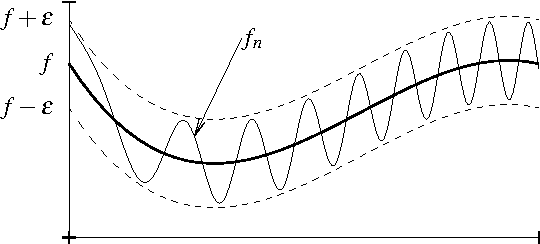
\includegraphics{figures/uniformconv}
\caption{In uniform convergence,
for $n \geq N$,
the functions $f_n$ are within a strip of $\pm\epsilon$ from $f$.%
\label{fig:uniformconv}}
\end{myfig}

It can easily be seen that uniform convergence implies pointwise
convergence.  The converse does not hold.

\begin{exbox}
\begin{exercise}
Prove that on $[0,1]$, the functions $x^n$ converge
pointwise but not uniformly.
\end{exercise}
\end{exbox}

\begin{defn} \label{def:unifnorm}
Let $f \colon S \to \R$ be a bounded function.  Define
\glsadd{not:uniformnorm}
\begin{equation*}
\norm{f}_S
\overset{\text{def}}{=}
\sup \bigl\{ \abs{f(x)} : x \in S \bigr\} .
\end{equation*}
$\norm{\cdot}_S$ is called the \emph{\myindex{uniform norm}}.
\end{defn}

\begin{prop}
A sequence of bounded functions $f_n \colon S \to \R$ converges
uniformly to $f \colon S \to \R$, if and only if
\begin{equation*}
\lim_{n\to\infty} \norm{f_n - f}_S = 0 .
\end{equation*}
\end{prop}

\begin{exbox}
\begin{exercise}
Prove the proposition.
\end{exercise}
\end{exbox}

Sometimes we say that \emph{$\{ f_n \}$ converges to $f$ in uniform norm}
\index{converges in uniform norm}
\index{uniform norm convergence}
instead of \emph{converges uniformly}.  The proposition
says that the two notions are the same thing.

Using uniform norm, we define Cauchy sequences in a similar way
as we define Cauchy sequences of real numbers.

\begin{defn}
Let $f_n \colon S \to \R$ be bounded functions.
The sequence is \emph{\myindex{Cauchy in the uniform norm}}
or \emph{\myindex{uniformly Cauchy}}
if for every $\epsilon > 0$, there exists an $N \in \N$ such
that for $m,k \geq N$ we have
\begin{equation*}
\norm{f_m-f_k}_S < \epsilon .
\end{equation*}
\end{defn}

\begin{prop} \label{prop:uniformcauchy}
Let $f_n \colon S \to \R$ be bounded functions.
Then $\{ f_n \}$ is Cauchy in the uniform norm if and only if
there exists an $f \colon S \to \R$ and $\{ f_n \}$ converges
uniformly to $f$.
\end{prop}

\begin{proof}
Let us first suppose $\{ f_n \}$ is Cauchy in the uniform norm.
Let us define $f$.  Fix $x$, then
the sequence $\{ f_n(x) \}$ is Cauchy because
\begin{equation*}
\abs{f_m(x)-f_k(x)}
\leq
\norm{f_m-f_k}_S .
\end{equation*}
Thus $\{ f_n(x) \}$ converges to some real number.  Define $f \colon S
\to \R$ by
\begin{equation*}
f(x) = \lim_{n \to \infty} f_n(x) .
\end{equation*}
The sequence
$\{ f_n \}$ converges pointwise to $f$.  To show that the convergence
is uniform, let $\epsilon > 0$ be given.  Find an $N$ such that
for $m, k \geq N$ we have
$\norm{f_m-f_k}_S < \nicefrac{\epsilon}{2}$.  In other words for
all $x$ we have
$\abs{f_m(x)-f_k(x)} < \nicefrac{\epsilon}{2}$.  We take the limit
as $k$ goes to infinity.  Then $\abs{f_m(x)-f_k(x)}$
goes to $\abs{f_m(x)-f(x)}$.
Consequently for all $x$ we get
\begin{equation*}
\abs{f_m(x)-f(x)} \leq \nicefrac{\epsilon}{2} < \epsilon .
\end{equation*}
And hence $\{ f_n \}$ converges uniformly.

For the other direction, suppose $\{ f_n \}$ converges uniformly to
$f$.  Given $\epsilon > 0$, find $N$ such that for all $n \geq N$,
$\abs{f_n(x)-f(x)} < \nicefrac{\epsilon}{4}$ for all $x \in S$.
Therefore for all $m, k \geq N$,
\begin{equation*}
\abs{f_m(x)-f_k(x)}
%= 
%\abs{f_m(x)-f(x)+f(x)-f_k(x)}
\leq
\abs{f_m(x)-f(x)}+\abs{f(x)-f_k(x)} < \nicefrac{\epsilon}{4} +
\nicefrac{\epsilon}{4} .
\end{equation*}
Take supremum over all $x$ to obtain
\begin{equation*}
\norm{f_m-f_k}_S \leq \nicefrac{\epsilon}{2} < \epsilon .  \qedhere
\end{equation*}
\end{proof}

\begin{exbox}
\begin{exercise}
Let $f$ and $g$ be bounded functions on $[a,b]$.  Prove 
\begin{equation*}
\norm{f+g}_S \leq \norm{f}_S + \norm{g}_S .
\end{equation*}
\end{exercise}

\begin{exercise}
\begin{exparts}
\item
Find the pointwise limit $\dfrac{e^{x/n}}{n}$ for $x \in \R$.
\item
Is the limit uniform on $\R$?
\item
Is the limit uniform on $[0,1]$?
\end{exparts}
\end{exercise}

\begin{exercise}
Suppose $f_n \colon S \to \R$ are functions that converge uniformly
to $f \colon S \to \R$.  Suppose $A \subset S$.  Show that
the sequence of restrictions $\{ f_n|_A \}$ converges uniformly to $f|_A$.
\end{exercise}

\begin{exercise}
\begin{exparts}
\item
Suppose $\{ f_n \}$ and $\{ g_n \}$ defined on some set $A$ converge to
$f$ and $g$ respectively pointwise, and let $a,b \in \R$.
Show that $\{ a f_n+ b g_n \}$ converges
pointwise to $a f+ b g$.
\item
Show the same for uniform convergence.
\end{exparts}
\end{exercise}

\begin{exercise}
Find an example of a sequence of functions $\{ f_n \}$ and $\{ g_n \}$
that converge uniformly to some $f$ and $g$ on some set $A$, but such that
$\{ f_ng_n \}$ (the multiple) does not converge uniformly to $fg$ on $A$.
\end{exercise}

\begin{exercise}
Suppose there exists a sequence of functions $\{ g_n \}$ uniformly
converging to $0$ on $A$.  Now suppose we have a sequence of functions
$\{ f_n \}$ and a function $f$ on $A$ such that
\begin{equation*}
\abs{f_n(x) - f(x)} \leq g_n(x) 
\end{equation*}
for all $x \in A$.  Show that $\{ f_n \}$ converges uniformly to $f$ on $A$.
\end{exercise}

\begin{exercise}
Let $\{ f_n \}$, $\{ g_n \}$ and $\{ h_n \}$ be sequences of functions on
$[a,b]$.  Suppose $\{ f_n \}$ and $\{ h_n \}$ converge uniformly to some function
$f \colon [a,b] \to \R$ and suppose $f_n(x) \leq g_n(x) \leq h_n(x)$
for all $x \in [a,b]$.  Show that $\{ g_n \}$ converges uniformly to $f$.
\end{exercise}

\begin{exercise}
Fix a continuous $h \colon [a,b] \to \R$.
Let $f(x) = h(x)$ for $x \in [a,b]$,
$f(x) = h(a)$ for $x < a$ and $f(x) = h(b)$ for all $x > b$.  First show
that $f \colon \R \to \R$ is continuous.
Let
\begin{equation*}
f_n(x) = \frac{n}{2} \int_{x-1/n}^{x+1/n} f(t) \, dt .
\end{equation*}
Show that $\{ f_n \}$ converges uniformly to $h$ on $[a,b]$.
\end{exercise}


\begin{exercise}
Prove that
if a sequence of functions $f_n \colon S \to \R$
converge uniformly to a bounded function $f \colon S \to \R$,
then there exists an $N$ such that for all $n \geq N$, the $f_n$
are bounded.
\end{exercise}

\begin{exercise}
In \exampleref{example:geomsumptconv} we saw
$\sum_{k=0}^\infty x^k$ converges pointwise to $\frac{1}{1-x}$ on
$(-1,1)$.
\begin{exparts}
\item
Show that for any $0 \leq c < 1$, the series
$\sum_{k=0}^\infty x^k$ converges uniformly on $[-c,c]$.
\item
Show that the series $\sum_{k=0}^\infty x^k$ does not converge uniformly
on $(-1,1)$.
\end{exparts}
\end{exercise}
\end{exbox}

\subsection{Continuity of the limit}

If we have a sequence $\{ f_n \}$ of continuous functions,
is the limit continuous?  We have seen that for pointwise
convergence, this need not be the case.
If we, however, require the convergence to be uniform, the limits can
be interchanged.

\begin{thm}
Let $\{ f_n \}$ be 
a sequence of continuous functions $f_n \colon S \to \R$ converging
uniformly to  $f \colon S \to \R$.  Then $f$ is continuous.
\end{thm}

\begin{proof}
Let $x \in S$ be fixed.  Let $\{ x_n \}$ be a sequence in $S$
converging to $x$.

Let $\epsilon > 0$ be given.
As $\{ f_k \}$ converges uniformly to $f$, we find a $k \in \N$ such that
\begin{equation*}
\abs{f_k(y)-f(y)} < \nicefrac{\epsilon}{3}
\end{equation*}
for all $y \in S$.  As $f_k$ is continuous at $x$,
we find an $N \in \N$ such that for $m \geq N$
we have 
\begin{equation*}
\abs{f_k(x_m)-f_k(x)} < \nicefrac{\epsilon}{3} .
\end{equation*}
Thus for
$m \geq N$ we have
\begin{equation*}
\begin{split}
\abs{f(x_m)-f(x)}
& =
\abs{f(x_m)-f_k(x_m)+f_k(x_m)-f_k(x)+f_k(x)-f(x)}
\\
& \leq
\abs{f(x_m)-f_k(x_m)}+
\abs{f_k(x_m)-f_k(x)}+
\abs{f_k(x)-f(x)}
\\
& <
\nicefrac{\epsilon}{3} +
\nicefrac{\epsilon}{3} +
\nicefrac{\epsilon}{3} = \epsilon .
\end{split}
\end{equation*}
Therefore $\{ f(x_m) \}$ converges to $f(x)$ and hence $f$ is continuous at
$x$.  As $x$ was arbitrary, $f$ is continuous everywhere.
\end{proof}

\begin{exbox}
\begin{exercise}
We say that a sequence of functions $f_n \colon \R \to \R$
\emph{\myindex{converges uniformly on compact subsets}}
\index{uniform convergence on compact subsets}
if for every $k \in \N$,
the sequence $\{ f_n \}$ converges uniformly on $[-k,k]$.
\begin{exparts}
\item
Prove that if $f_n \colon \R \to \R$ is a sequence of
continuous functions converging uniformly on compact subsets, then
the limit is continuous.
\item 
Prove that if $f_n \colon \R \to \R$ is a sequence of
functions Riemann integrable on any closed and bounded interval $[a,b]$,
and converging uniformly on compact subsets to an $f \colon \R \to \R$,
then for any interval $[a,b]$, we have $f \in \sR[a,b]$, and
$\int_a^b f = \lim_{n\to\infty} \int_a^b f_n$.
\end{exparts}
\end{exercise}
\end{exbox}

\subsection{Integral of the limit}

Again, if we simply require pointwise convergence, then the integral
of a limit of a sequence of functions need not be equal to the limit
of the integrals.

\begin{example}
Let $\chi_{T}$ be the characteristic function of a set $T$, that is $\chi_T(x) =
1$ if $x \in T$ and $\chi_T(x) = 0$ otherwise.
The functions $n \chi_{(0,\nicefrac{1}{n})}$ all integrate (on the interval
$[0,1]$) to 1.  Their
pointwise limit limit is 0 (whose integral is 0).
\end{example}

If we require the convergence to be uniform, the limits can
be interchanged.

\begin{thm} \label{integralinterchange:thm}
Let $\{ f_n \}$ be a sequence of Riemann integrable
functions
$f_n \colon [a,b] \to \R$
converging uniformly to $f \colon [a,b]
\to \R$.  Then $f$ is Riemann integrable and
\begin{equation*}
\int_a^b f(x) \, dx = \lim_{n\to\infty} \int_a^b f_n(x) \, dx .
\end{equation*}
\end{thm}

In the following, let 
$\overline{\int_a^b} f(x)\, dx$ and 
$\underline{\int_a^b} f(x)\, dx$ denote the upper and lower Darboux integral.
The definition of the Riemann integral using Darboux sums and integrals is
beyond the scope of this book, but let us just mention that 
if the upper and lower Darboux integrals are equal, then a function is
Riemann integrable, and the common value is the integral.  Given this,
let us prove the theorem.

\begin{proof}
Let $\epsilon > 0$ be given.
As $f_n$ goes to $f$ uniformly, we find an $M \in \N$ such that
for all $n \geq M$ we have 
$\abs{f_n(x)-f(x)} < \frac{\epsilon}{2(b-a)}$ for all $x \in [a,b]$.
In particular, by reverse triangle inequality
$\abs{f(x)} < \frac{\epsilon}{2(b-a)} + \abs{f_n(x)}$ for all $x$,
hence $f$ is bounded
as $f_n$ is bounded.
Note that $f_n$ is integrable and compute
\begin{equation*}
\begin{split}
\overline{\int_a^b} & f(x) \, dx
-
\underline{\int_a^b} f(x) \, dx
\\
& =
\overline{\int_a^b} \bigl( f(x) - f_n(x) + f_n(x) \bigr) \, dx
-
\underline{\int_a^b} \bigl( f(x) - f_n(x) + f_n(x) \bigr) \, dx
\\
& \leq
\overline{\int_a^b} \bigl( f(x) - f_n(x) \bigr) \, dx +  \overline{\int_a^b}
f_n(x) \, dx
-
\underline{\int_a^b} \bigl( f(x) - f_n(x) \bigr) \, dx -
\underline{\int_a^b} f_n(x) \, dx
\\
& =
\overline{\int_a^b} \bigl( f(x) - f_n(x) \bigr)\, dx +  \int_a^b f_n(x) \, dx
-
\underline{\int_a^b} \bigl( f(x) - f_n(x) \bigr)\, dx -  \int_a^b f_n(x) \, dx
\\
& =
\overline{\int_a^b} \bigl( f(x) - f_n(x) \bigr)\, dx
-
\underline{\int_a^b} \bigl( f(x) - f_n(x) \bigr)\, dx
\\
& \leq
\frac{\epsilon}{2(b-a)} (b-a) + 
\frac{\epsilon}{2(b-a)} (b-a) = \epsilon .
\end{split}
\end{equation*}
The second inequality follows from
the fact that for all $x \in [a,b]$ we have
$\frac{-\epsilon}{2(b-a)} < f(x)-f_n(x) < \frac{\epsilon}{2(b-a)}$.
As $\epsilon > 0$ was arbitrary, $f$ is Riemann integrable.

We compute $\int_a^b f(x)\,dx$.
For $n \geq M$ ($M$ is the same as above),
\begin{equation*}
\begin{split}
\abs{\int_a^b f(x)\,dx - \int_a^b f_n(x)\,dx} & = 
\abs{ \int_a^b \bigl(f(x) - f_n(x)\bigr)\,dx}
\\
& \leq
\frac{\epsilon}{2(b-a)} (b-a) = \frac{\epsilon}{2} < \epsilon .
\end{split}
\end{equation*}
Therefore $\bigl\{ \int_a^b f_n(x) \,dx \bigr\}$ converges to $\int_a^b f(x) \,dx$.
\end{proof}

\begin{example}
Using \thmref{integralinterchange:thm}, we compute
\begin{equation*}
\lim_{n\to\infty} \int_0^1 \frac{nx+ \sin(nx^2)}{n} \,dx
=
\int_0^1
x \,dx = \nicefrac{1}{2} .
\end{equation*}
It is impossible to compute the integrals for any particular $n$ using 
calculus as $\sin(nx^2)$ has no closed-form antiderivative.
\end{example}

\begin{remark}
While we will not require the Lebesgue integral in this book, note that
for Lebesgue integral a much stronger convergence theorem holds.  In
particular, the Dominated Convergence Theorem implies that if
$\{ f_n \}$ is a sequence of measurable functions on $[a,b]$,
converging pointwise to $f \colon [a,b] \to \R$, and such that
$\{ f_n \}$ is uniformly bounded (there is a single $B \in \R$ such that
$\snorm{f_n}_{[a,b]} \leq B$ for all $n$), then
\begin{equation*}
\int_a^b f(x) \, dx = \lim_{n\to\infty} \int_a^b f_n(x) \, dx .
\end{equation*}
Where of course all the integrals would have to be the Lebesgue integrals,
not the Riemann integrals.  The pointwise limit of Riemann integrable
functions need not even be Riemann integrable.
\end{remark}

\begin{exbox}
\begin{exercise}
Compute
$\displaystyle \lim_{n\to\infty} \int_1^2 e^{-nx^2} ~dx$.
\end{exercise}

\begin{exercise}
Find a sequence of Riemann integrable functions $f_n \colon [0,1] \to \R$ such
that $\{ f_n \}$ converges to zero pointwise, and such that
\begin{exparts}
\item
$\bigl\{ \int_0^1 f_n(x)\,dx \bigr\}_{n=1}^\infty$ increases without bound,
\item
$\bigl\{ \int_0^1 f_n(x)\,dx \bigr\}_{n=1}^\infty$ is the sequence $-1,1,-1,1,-1,1, \ldots$.
\end{exparts}
\end{exercise}
\end{exbox}

\subsection{Derivative of the limit}

While uniform convergence is enough to swap limits with integrals, it is not,
however, enough to swap limits with derivatives, unless you also have
uniform convergence of the derivatives themselves.

\begin{example}
Let $f_n(x) = \frac{\sin(nx)}{n}$.  Then $f_n$ converges uniformly to
0.  See \figureref{fig:conv1nsinxn}.
The derivative of the limit is 0.  But $f_n'(x) = \cos(nx)$, which
does not converge even pointwise, for
example $f_n'(\pi) = {(-1)}^n$.  Furthermore,
$f_n'(0) = 1$ for all $n$, which does converge, but not to 0.
\begin{myfig}
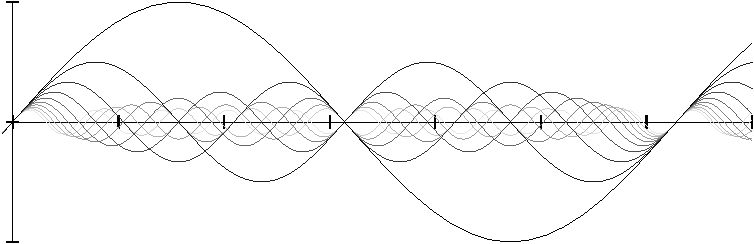
\includegraphics{figures/conv1nsinxn}
\caption{Graphs of $\frac{\sin(nx)}{n}$ for
$n=1,2,\ldots,10$, with higher $n$ in lighter gray.%
\label{fig:conv1nsinxn}}
\end{myfig}
\end{example}

The following theorem is true even if 
we do not assume continuity of the derivatives, but the proof is more
difficult.

\begin{thm} \label{thm:dersconverge}
Let $I$ be a bounded interval and let
$f_n \colon I \to \R$ be continuously differentiable functions.
Suppose $\{ f_n' \}$ converges uniformly to $g \colon I \to \R$,
and suppose $\{ f_n(c) \}_{n=1}^\infty$ is a
convergent sequence for some $c \in I$.  Then $\{ f_n \}$ converges uniformly to 
a continuously differentiable function $f \colon I \to \R$, and $f' = g$.
\end{thm}

\begin{proof}
Define $f(c) = \lim_{n\to \infty} f_n(c)$.
As $f_n'$ are continuous and hence Riemann integrable,
then
via the Fundamental Theorem of Calculus, we find that for $x \in I$,
\begin{equation*}
f_n(x) = f_n(c) + \int_c^x f_n' (t)\, dt.
\end{equation*}
As $\{ f_n' \}$ converges uniformly on $I$, it converges uniformly
on $[c,x]$ (or $[x,c]$ if $x < c$).
Therefore, we find that the limit on the right hand side exists.
Let us define $f$ at the remaining points by this limit:
\begin{equation*}
f(x) =
\lim_{n\to\infty} f_n(c) + \lim_{n\to\infty} \int_c^x f_n' (t)\, dt
=
f(c) + \int_c^x g(t)\,dt .
\end{equation*}
The function $g$ is continuous, being the uniform limit of continuous
functions.  Hence $f$ is differentiable and $f'(x) = g(x)$ for all $x \in I$
by the second form of the fundamental theorem.

It remains to prove
uniform convergence.
Suppose $I$ has a lower bound $a$ and upper bound $b$.
Let $\epsilon > 0$ be given.  Take $M$
such that for $n \geq M$ we have
$\abs{f(c)-f_n(c)} < \nicefrac{\epsilon}{2}$,
and
$\abs{g(x)-f_n'(x)} < \nicefrac{\epsilon}{2(b-a)}$
for all $x \in I$.  Then
\begin{equation*}
\begin{split}
\abs{f(x) - f_n(x)} & =
\abs{f(c) + \int_c^x g - f_n(c) - \int_c^x f_n'(t)\,dt}
\\
& \leq
\abs{f(c) - f_n(c)} + \abs{\int_c^x g(t)\,dt - \int_c^x f_n'(t)\,dt}
\\
& =
\abs{f(c) - f_n(c)} + \abs{\int_c^x \bigl(g(t) - f_n'(t)\bigr) \, dt}
\\
& <
\frac{\epsilon}{2}
+
\frac{\epsilon}{2(b-a)}
(b-a)
=\epsilon. \qedhere
\end{split}
\end{equation*}
\end{proof}

The proof goes through without boundedness of $I$, except for the
uniform convergence of $f_n$ to $f$.  As an example suppose $I = \R$ and let
$f_n(x) = \nicefrac{x}{n}$.  Then $f_n'(x)=\nicefrac{1}{n}$, which
converges uniformly to $0$.  However, $\{f_n\}$ converges to 0 only pointwise.

\begin{exbox}
\begin{exercise}
Find an explicit example of a sequence of
differentiable functions on $[-1,1]$ that converge uniformly to
a function $f$ such that $f$ is not differentiable.
Hint:
There are many possibilities,
simplest is perhaps to combine $\abs{x}$ and $\frac{n}{2}x^2 +
\frac{1}{2n}$, another is to
consider $\sqrt{x^2+{(\nicefrac{1}{n})}^2}$.  Show that these functions are differentiable,
converge uniformly, and then show that the limit is not differentiable.
\end{exercise}

\begin{exercise}
Let $f_n(x) = \frac{x^n}{n}$.  Show that $\{ f_n \}$ converges uniformly to
a differentiable function $f$ on $[0,1]$ (find $f$).  However, show that
$f'(1) \not= \lim\limits_{n\to\infty} f_n'(1)$.
\end{exercise}
\end{exbox}

%%%%%%%%%%%%%%%%%%%%%%%%%%%%%%%%%%%%%%%%%%%%%%%%%%%%%%%%%%%%%%%%%%%%%%%%%%%%%%

\section{Continuity and derivatives under the integral}
\label{sec:contlimitsunderint}

\subsection{Continuity}

Let us prove a useful criterion for
continuity of functions defined by integrals.  Let $f(x,y)$ be a function of two variables and define
\begin{equation*}
g(y) = \int_a^b f(x,y) \,dx .
\end{equation*}
Question is, is $g$ is continuous?
We are really asking when do two limiting operations commute,
which is not always possible, so some extra hypothesis
is necessary.  A useful sufficient (but not
necessary) condition is that $f$ is continuous on a closed rectangle.

\begin{prop} \label{prop:integralcontcont}
If $f \colon [a,b] \times [c,d] \to \R$ is a continuous function,
then $g \colon [c,d] \to \R$ defined by
\begin{equation*}
g(y) = \int_a^b f(x,y) \,dx  \qquad \text{is continuous}.
\end{equation*}
\end{prop}

\begin{proof}
Fix $y \in [c,d]$, and let $\{ y_n \}$ be a sequence in $[c,d]$
converging to $y$.
Let $\epsilon > 0$ be given.
As $f$ is continuous on $[a,b] \times [c,d]$, which is compact, $f$
is uniformly continuous.  
In particular, there exists a $\delta > 0$ such that
whenever $\widetilde{y} \in [c,d]$ and
$\abs{\widetilde{y}-y} < \delta$ we have
$\abs{f(x,\widetilde{y})-f(x,y)} < \epsilon$ for all $x \in [a,b]$.
If we let $h_n(x)= f(x,y_n)$ and $h(x) = f(x,y)$,
we have just shown that
$h_n \colon [a,b] \to \R$ converges uniformly 
to
$h \colon [a,b] \to \R$ as $n$ goes to $\infty$.
Uniform convergence implies the limit can be taken underneath the integral.
So
\begin{equation*}
\lim_{n\to \infty}
g(y_n)
=
\lim_{n\to \infty}
\int_a^b 
f(x,y_n) \,dx 
= 
\int_a^b 
\lim_{n\to \infty}
f(x,y_n) \,dx 
= 
\int_a^b 
f(x,y) \,dx = g(y) . \qedhere
\end{equation*}
\end{proof}

In applications, if we are interested in continuity at $y_0$, we just
need to apply the proposition in $[a,b] \times [y_0-\epsilon,y_0+\epsilon]$
for some small $\epsilon > 0$.  For example, if $f$ is continuous in
$[a,b] \times \R$, then $g$ is continuous on $\R$.

\begin{exbox}
\begin{exercise} \label{exercise:integralcontcontextra}
Prove a stronger version of \propref{prop:integralcontcont}:
If $f \colon (a,b) \times (c,d) \to \R$ is a bounded continuous function,
then $g \colon [c,d] \to \R$ defined by
\begin{equation*}
g(y) = \int_a^b f(x,y) \,dx  \qquad \text{is continuous}.
\end{equation*}
Hint: First integrate over $[a+\nicefrac{1}{n},b-\nicefrac{1}{n}]$.
\end{exercise}
\end{exbox}

\subsection{Differentiation under the integral}
\label{subsec:diffunderint}

Let $f(x,y)$ be a function of two variables and
\begin{equation*}
g(y) = \int_a^b f(x,y) \,dx .
\end{equation*}
If $f$ is continuous on the compact rectangle $[a,b] \times [c,d]$, then
\propref{prop:integralcontcont}
says that $g$ is continuous on $[c,d]$.

Suppose $f$ is differentiable in $y$.  The main question we want to
ask is when can we ``differentiate under the integral,'' that is,
when is it true that $g$ is differentiable and its derivative is
\begin{equation*}
g'(y) \overset{?}{=} \int_a^b \frac{\partial f}{\partial y}(x,y) \,dx .
\end{equation*}
Differentiation is a limit and therefore we are really asking when do the
two limiting operations of integration and differentiation commute.
This is not always possible and some extra hypothesis is
necessary.  In particular, the first
question we would face is the integrability of
$\frac{\partial f}{\partial y}$, but the formula can fail even if
$\frac{\partial f}{\partial y}$ is integrable as a function of $x$ for every
fixed $y$.

Let us prove a simple, but perhaps the most useful version of this theorem.

\begin{thm}[\myindex{Leibniz Integral Rule}]
Suppose $f \colon [a,b] \times [c,d] \to \R$ is a continuous function,
such that $\frac{\partial f}{\partial y}$ exists for all $(x,y) \in [a,b]
\times [c,d]$ and is continuous.  Define
\begin{equation*}
g(y) = \int_a^b f(x,y) \,dx .
\end{equation*}
Then $g \colon [c,d] \to \R$ is continuously differentiable and
\begin{equation*}
g'(y) = \int_a^b \frac{\partial f}{\partial y}(x,y) \,dx .
\end{equation*}
\end{thm}

The hypotheses on $f$ and $\frac{\partial f}{\partial y}$ can be
weakened, see e.g.\ \exerciseref{exercise:strongerleibniz},
but not dropped outright.
The main point in the proof is for
$\frac{\partial f}{\partial y}$ to exist and be continuous for all $x$
up to the ends, but we only need a small
interval in the $y$ direction.  In applications, we often make $[c,d]$ be a
small interval around the point where we need to differentiate.

\begin{proof}
Fix $y \in [c,d]$ and let $\epsilon > 0$ be given.
As $\frac{\partial f}{\partial y}$ is continuous on $[a,b] \times [c,d]$ it
is uniformly continuous.  In particular, there exists $\delta > 0$ such that
whenever $y_1 \in [c,d]$ with
$\abs{y_1-y} < \delta$ and all $x \in [a,b]$ we have
\begin{equation*}
\abs{\frac{\partial f}{\partial y}(x,y_1)-\frac{\partial f}{\partial y}(x,y)} < \epsilon .
\end{equation*}

Suppose $h$ is such that $y+h \in [c,d]$ and $\abs{h} < \delta$.
Fix $x$ for a moment
and apply the Mean Value Theorem to find a $y_1$ between $y$ and $y+h$ such that
\begin{equation*}
\frac{f(x,y+h)-f(x,y)}{h}
=
\frac{\partial f}{\partial y}(x,y_1) .
\end{equation*}
As $\abs{y_1-y} \leq \abs{h} < \delta$,
\begin{equation*}
\abs{
\frac{f(x,y+h)-f(x,y)}{h}
-
\frac{\partial f}{\partial y}(x,y) 
}
=
\abs{
\frac{\partial f}{\partial y}(x,y_1) 
-
\frac{\partial f}{\partial y}(x,y) 
}
< \epsilon .
\end{equation*}
This argument worked for every $x \in [a,b]$.  Therefore, as a function of
$x$
\begin{equation*}
x \mapsto \frac{f(x,y+h)-f(x,y)}{h}
\quad
\text{converges uniformly to}
\quad
x \mapsto \frac{\partial f}{\partial y}(x,y)
\quad
\text{as $h \to 0$} .
\end{equation*}
We defined uniform convergence for sequences although the idea is the
same.  You may replace $h$ with a sequence of nonzero 
numbers $\{ h_n \}$
converging to $0$ such that $y+h_n \in [c,d]$ and let $n \to \infty$.

Consider the difference quotient of $g$,
\begin{equation*}
\frac{g(y+h)-g(y)}{h}
=
\frac{\int_a^b f(x,y+h) \,dx -
\int_a^b f(x,y) \,dx }{h}
=
\int_a^b \frac{f(x,y+h)-f(x,y)}{h} \,dx .
\end{equation*}
Uniform convergence implies the limit can be taken underneath the integral.
So
\begin{equation*}
\lim_{h\to 0}
\frac{g(y+h)-g(y)}{h}
= 
\int_a^b 
\lim_{h\to 0}
\frac{f(x,y+h)-f(x,y)}{h} \,dx 
=
\int_a^b 
\frac{\partial f}{\partial y}(x,y) \,dx .
\end{equation*}
Then $g'$ is continuous on $[c,d]$ by
\propref{prop:integralcontcont}.
\end{proof}

\begin{example} \label{example:counterexamplediffunder}
Suppose we start with
\begin{equation*}
\int_0^{1} \frac{x-1}{\ln(x)} \,dx .
\end{equation*}
The function under the integral 
extends to be continuous on $[0,1]$, and hence
the integral exists, see \exerciseref{exercise:counterexamplediffunder}.  Trouble is finding it.  Introduce a parameter $y$
and define a function:
\begin{equation*}
g(y) = \int_0^{1} \frac{x^y-1}{\ln(x)} \,dx .
\end{equation*}
The function
$\frac{x^y-1}{\ln(x)}$
also extends to a continuous function of $x$ and $y$
for $(x,y) \in [0,1] \times [0,1]$ (also in the exercise).
See \figureref{fig:diffunderexample}.
\begin{myfig}
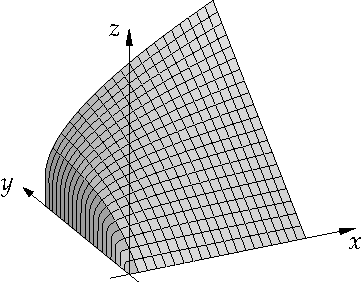
\includegraphics{figures/diffunderexample}
\caption{The graph $z= \frac{x^y-1}{\ln(x)}$ on $[0,1] \times [0,1]$.\label{fig:diffunderexample}}
\end{myfig}


Therefore
$g$ is a continuous function of on $[0,1]$, and $g(0) = 0$.
For any $\epsilon > 0$, the $y$ derivative of the integrand, $x^y$,
is continuous on $[0,1] \times [\epsilon,1]$.  Therefore,
for $y >0$ we may differentiate under the integral sign
\begin{equation*}
g'(y) =
\int_0^{1} \frac{\ln(x) x^y}{\ln(x)} \,dx 
=
\int_0^{1} x^y \,dx =
\frac{1}{y+1} .
\end{equation*}
We need to figure out $g(1)$, knowing $g'(y) = \frac{1}{y+1}$ and $g(0) =
0$.  By elementary calculus we find $g(1) = \int_0^1 g'(y)\,dy = \ln(2)$.  Therefore
\begin{equation*}
\int_0^{1} \frac{x-1}{\ln(x)} \,dx  = \ln(2).
\end{equation*}
\end{example}

\begin{exbox}
\begin{samepage}
\begin{exercise} \label{exercise:counterexamplediffunder}
Prove the two statements that were asserted in
\exampleref{example:counterexamplediffunder}:
\begin{exparts}
\item
Prove $\frac{x-1}{\ln(x)}$ extends to a continuous function of
$[0,1]$.  That is, there exists a continuous function on $[0,1]$
that equals $\frac{x-1}{\ln(x)}$ on $(0,1)$.
\item
Prove $\frac{x^y-1}{\ln(x)}$ extends to a continuous function
on $[0,1] \times [0,1]$.
\end{exparts}
\end{exercise}
\end{samepage}

\begin{exercise}
Suppose $h \colon \R \to \R$ is a continuous function.  Suppose $g
\colon \R \to \R$ is which is continuously differentiable and compactly
supported.  That is there exists some $M > 0$ such that $g(x) = 0$ whenever
$\abs{x} \geq M$.  Define
\begin{equation*}
f(x) = \int_{-\infty}^\infty h(y)g(x-y) \, dy  .
\end{equation*}
Show that $f$ is differentiable.
\end{exercise}

\begin{exercise}
Suppose $f \colon \R \to \R$ is an infinitely differentiable function (all derivatives exist)
such that $f(0) = 0$.  Then show that there exists an infinitely
differentiable function $g \colon \R \to \R$ such that $f(x) = x\,g(x)$.  Finally show that
if $f'(0) \not= 0$, then $g(0) \not= 0$.\\
Hint: First write
$f(x) = \int_0^x f'(s) \,ds$ and then rewrite the integral to go
from $0$ to $1$.
\end{exercise}

\begin{exercise}
Let $U \subset \R^n$ be an open set and suppose
$f(x,y_1,y_2,\ldots,y_n)$ is a continuous
function defined on $[0,1] \times U \subset \R^{n+1}$.
Suppose
$\frac{\partial f}{\partial y_1},
\frac{\partial f}{\partial y_2},\ldots,
\frac{\partial f}{\partial y_n}$
exist and are continuous on $[0,1] \times U$.
Then prove that $F \colon U \to \R$ defined by
\begin{equation*}
F(y_1,y_2,\ldots,y_n) =
\int_0^1
f(x,y_1,y_2,\ldots,y_n)
\, dx
\end{equation*}
is continuously differentiable.
\end{exercise}

\begin{exercise}
Work out the following counterexample:  Let
\begin{equation*}
f(x,y) =
\begin{cases}
\frac{xy^3}{{(x^2+y^2)}^2} & \text{if $x\not=0$ or $y\not= 0$,}\\
0 & \text{if $x=0$ and $y=0$.}
\end{cases}
\end{equation*}
\begin{exparts}
\item
Prove that for any fixed $y$ the function $x \mapsto f(x,y)$ is
Riemann integrable on $[0,1]$ and
\begin{equation*}
g(y) = \int_0^1 f(x,y) \, dx = \frac{y}{2y^2+2} .
\end{equation*}
Therefore $g'(y)$ exists and we get the continuous function
\begin{equation*}
g'(y) = \frac{1-y^2}{2{(y^2+1)}^2} .
\end{equation*}
\item
Prove $\frac{\partial f}{\partial y}$ exists at all $x$ and $y$ and
compute it.
\item
Show that for all $y$
\begin{equation*}
\int_0^1 \frac{\partial f}{\partial y} (x,y) \, dx
\end{equation*}
exists, but
\begin{equation*}
g'(0) \not= \int_0^1 \frac{\partial f}{\partial y} (x,0) \, dx .
\end{equation*}
\end{exparts}
\end{exercise}

\pagebreak[2]
\begin{exercise}
Work out the following counterexample:  Let
\begin{equation*}
f(x,y) =
\begin{cases}
x \,\sin \left(\frac{y}{x^2+y^2}\right) & \text{if $(x,y) \not= (0,0)$,}\\
0 & \text{if $(x,y)=(0,0)$.}
\end{cases}
\end{equation*}
\begin{exparts}
\item
Prove $f$ is continuous on all of $\R^2$.
Therefore the following function is well defined for every $y \in \R$:
\begin{equation*}
g(y) = \int_0^1 f(x,y) \, dx .
\end{equation*}
\item
Prove $\frac{\partial f}{\partial y}$ exists for all $(x,y)$,
but is not continuous at $(0,0)$.
\item
Show that $\int_0^1 \frac{\partial f}{\partial y}(x,0) \, dx$ does not
exist even if we take improper integrals, that is,
that the limit
$\lim\limits_{h \to 0^+} \int_h^1 \frac{\partial f}{\partial y}(x,0) \, dx$
does not exist.
\end{exparts}
Note: Feel free to use what you know about sine and cosine from calculus.
\end{exercise}

\begin{samepage}
\begin{exercise} \label{exercise:strongerleibniz}
Strengthen the Leibniz integral rule in the following way.
Suppose $f \colon (a,b) \times (c,d) \to \R$ is a bounded continuous function,
such that $\frac{\partial f}{\partial y}$ exists for all $(x,y) \in (a,b)
\times (c,d)$ and is continuous and bounded.  Define
\begin{equation*}
g(y) = \int_a^b f(x,y) \,dx .
\end{equation*}
Then $g \colon (c,d) \to \R$ is continuously differentiable and
\begin{equation*}
g'(y) = \int_a^b \frac{\partial f}{\partial y}(x,y) \,dx .
\end{equation*}
Hint: See also \exerciseref{exercise:integralcontcontextra} and
\thmref{thm:dersconverge}.
\end{exercise}
\end{samepage}
\end{exbox}

%%%%%%%%%%%%%%%%%%%%%%%%%%%%%%%%%%%%%%%%%%%%%%%%%%%%%%%%%%%%%%%%%%%%%%%%%%%%%%

\section{The derivative in several real variables} \label{sec:derinsv}

\subsection{The derivative}

In the following, the norm $\snorm{\cdot}$ of a vector in $\R^n$
is the Euclidean norm $\snorm{x} = \sqrt{x_1^2+\cdots+x_n^2}$.
When applied to a linear mapping (a matrix) it is the
\emph{\myindex{operator norm}}:
\begin{equation*}
\snorm{A} \overset{\text{def}}{=} \sup_{\snorm{x} = 1} \snorm{Ax} .
\end{equation*}
The following exercise collects some key facts about the operator norm
for the reader who has not seen this norm yet.

\begin{exbox}
\begin{exercise}
\begin{exparts} 
\item
Prove that if $A$ is a linear mapping between finite dimensional vector
spaces, then $\snorm{A} < \infty$.
\item
Prove that if $A$ is a linear mapping of vector spaces, then
$\snorm{Ax} \leq \snorm{A} \snorm{x}$.
\end{exparts} 
\end{exercise}
\end{exbox}

For a function $f \colon \R \to \R$, 
the derivative at $x$ exists if there
there is a number $a$ (the derivative of $f$ at $x$) such that
\begin{equation*}
\lim_{h \to 0} \abs{\frac{f(x+h)-f(x)}{h} - a} =
\lim_{h \to 0} \frac{\sabs{f(x+h)-f(x) - ah}}{\sabs{h}}
= 0.
\end{equation*}

Multiplying by $a$ is a linear map in one dimension:
$h \mapsto ah$.  Let us extend this idea to more variables.

\begin{defn}
Let $U \subset \R^n$ be an open subset and $f \colon U \to \R^m$.  We
say $f$ is \emph{(real) differentiable\index{real differentiable}}
at $x \in U$ if there exists
a linear $A \colon \R^n \to \R^m$ such that
\begin{equation*}
\lim_{\substack{h \to 0\\h\in \R^n}}
\frac{\snorm{f(x+h)-f(x) - Ah}}{\snorm{h}} = 0 .
\end{equation*}
We write $Df|_x = A$\glsadd{not:mvder} and
we say $A$ is the \emph{(real) derivative\index{real derivative}} of $f$ at $x$.
When $f$ is \emph{(real) differentiable} at
every $x \in U$, we say that $f$ is (real) differentiable.  See
\figureref{fig:svder}.
\end{defn}

\begin{myfig}
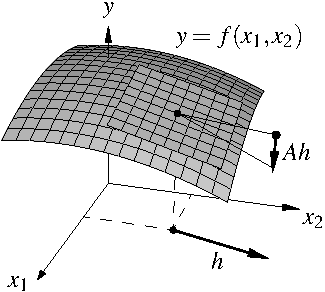
\includegraphics{figures/svder}
\caption{Illustration of a derivative for a function $f \colon \R^2 \to \R$.  The vector $h$ is shown
in the $x_1x_2$-plane based at $(x_1,x_2)$, and the vector
$Ah \in \R^1$ is shown along the $y$ direction.\label{fig:svder}}
\end{myfig}

We cheated somewhat and said that $A$
is \emph{the} derivative, let us prove that we were justified.

\begin{prop}
Let $U \subset \R^n$ be an open subset and $f \colon U \to \R^m$.  Suppose
$x \in U$ and there exist linear
$A,B \colon \R^n \to \R^m$ such that
\begin{equation*}
\lim_{h \to 0}
\frac{\snorm{f(x+h)-f(x) - Ah}}{\snorm{h}} = 0
\qquad \text{and} \qquad
\lim_{h \to 0}
\frac{\snorm{f(x+h)-f(x) - Bh}}{\snorm{h}} = 0 .
\end{equation*}
Then $A=B$.
\end{prop}

\begin{proof}
Suppose $h \in \R^n$, $h \not= 0$.  Compute
\begin{equation*}
\begin{split}
\frac{\snorm{(A-B)h}}{\snorm{h}} & =
\frac{\snorm{f(x+h)-f(x) - Ah - (f(x+h)-f(x) - Bh)}}{\snorm{h}} \\
& \leq
\frac{\snorm{f(x+h)-f(x) - Ah}}{\snorm{h}} + \frac{\snorm{f(x+h)-f(x) -
Bh}}{\snorm{h}} .
\end{split}
\end{equation*}
So 
$\frac{\snorm{(A-B)h}}{\snorm{h}} = \norm{(A-B)\frac{h}{\snorm{h}}} \to 0$
as $h \to 0$.  For an arbitrarily small $h$, $\frac{h}{\snorm{h}}$ is
on the unit sphere, and a linear mapping vanishing on the unit sphere is
zero everywhere.
\end{proof}

\begin{example}
If $f(x) = Ax$ for a linear mapping $A$, then
$Df|_x = A$:
\begin{equation*}
\frac{\snorm{f(x+h)-f(x) - Ah}}{\snorm{h}}
=
\frac{\snorm{A(x+h)-Ax - Ah}}{\snorm{h}}
=
\frac{0}{\snorm{h}} = 0 .
\end{equation*}
\end{example}

\begin{example}
Let $f \colon \R^2 \to \R^2$ be defined by
\begin{equation*}
f(x,y) = \bigl(f_1(x,y),f_2(x,y)\bigr) = (1+x+2y+x^2,2x+3y+xy).
\end{equation*}
Let us show that $f$ is differentiable at the origin and let us 
compute the derivative,
directly using the definition.  If the
derivative exists, it can be
represented by a $2$-by-$2$ matrix
$\left[\begin{smallmatrix}a&b\\c&d\end{smallmatrix}\right]$.  Suppose $h =
(h_1,h_2)$.  We need the following expression to go to zero.
\begin{multline*}
\frac{\snorm{
f(h_1,h_2)-f(0,0)
-
(ah_1 +bh_2 , ch_1+dh_2)}
}{\snorm{(h_1,h_2)}}
=
\\
\frac{\sqrt{
{\bigl((1-a)h_1 + (2-b)h_2 + h_1^2\bigr)}^2
+
{\bigl((2-c)h_1 + (3-d)h_2 + h_1h_2\bigr)}^2}}{\sqrt{h_1^2+h_2^2}} .
\end{multline*}
If we choose $a=1$, $b=2$, $c=2$, $d=3$, the expression becomes
\begin{equation*}
\frac{\sqrt{
h_1^4 + h_1^2h_2^2}}{\sqrt{h_1^2+h_2^2}}
=
\sabs{h_1}
\frac{\sqrt{
h_1^2 + h_2^2}}{\sqrt{h_1^2+h_2^2}}
= \sabs{h_1} .
\end{equation*}
And this expression does indeed go to zero as $h \to 0$.  The
function $f$ is differentiable at the origin and 
the derivative $Df|_0$ is represented by the matrix
$\left[\begin{smallmatrix}1&2\\2&3\end{smallmatrix}\right]$.
\end{example}

\begin{prop}
Let $U \subset \R^n$ be open and $f \colon U \to \R^m$ be
differentiable at $p \in U$.  Then $f$ is continuous at $p$.
\end{prop}

\begin{proof}
Another way to write the differentiability of $f$ at $p$ is to first write
\begin{equation*}
r(h) = f(p+h)-f(p) - Df|_p h ,
\end{equation*}
and $\frac{\snorm{r(h)}}{\snorm{h}}$ must go to zero as $h \to 0$.
So
$r(h)$ itself must go to zero.  The mapping $h \mapsto Df|_p h$
is a linear mapping between finite dimensional spaces, it is
therefore continuous
and goes to zero as $h \to 0$.  So
$f(p+h)$ must go to $f(p)$ as $h \to 0$.
\end{proof}

The derivative is itself a linear operator on the space of differentiable
functions.

\begin{prop}
Suppose $U \subset \R^n$ is open,
$f \colon U \to \R^m$ and
$g \colon U \to \R^m$ are differentiable at $p$,
and $\alpha \in \R$.  Then the functions $f+g$ and $\alpha f$
are differentiable at $p$ and
\begin{equation*}
D(f+g)|_p = Df|_p + Dg|_p , \qquad \text{and} \qquad D(\alpha f)|_p = \alpha
Df|_p .
\end{equation*}
\end{prop}

\begin{proof}
Let $h \in \R^n$, $h \not= 0$.  The proposition follows from the following
estimates:
\begin{multline*}
\frac{\norm{f(p+h)+g(p+h)-\bigl(f(p)+g(p)\bigr) - \bigl(Df|_p + Dg|_p\bigr)h}}{\snorm{h}}
\\
\leq
\frac{\norm{f(p+h)-f(p) - Df|_ph}}{\snorm{h}}
+
\frac{\norm{g(p+h)-g(p) - Dg|_ph}}{\snorm{h}} ,
\end{multline*}
and
\begin{equation*}
\frac{\norm{\alpha f(p+h) - \alpha f(p) - \alpha Df|_p h}}{\snorm{h}}
=
\sabs{\alpha} \frac{\norm{f(p+h))-f(p) - Df|_ph}}{\snorm{h}} .
\qedhere
\end{equation*}
\end{proof}

If $A \colon X \to Y$ and $B \colon Y \to Z$ are linear maps, then 
they are their own derivative.  The composition
$BA$, a linear map from $X$ to $Z$, is also its own derivative, and
so the derivative of the composition is the composition
of the derivatives.  As differentiable maps are ``infinitesimally close''
to linear maps, they have the same property:

\begin{thm}[Chain rule] \label{thm:realchain}
Let $U \subset \R^n$ be open and let $f \colon U \to \R^m$ be
differentiable at $p \in U$.  Let $V \subset \R^m$ be open,
$f(U) \subset V$ and let $g \colon V \to \R^\ell$ be differentiable
at $f(p)$.  Then
\begin{equation*}
F(x) = g\bigl(f(x)\bigr)
\end{equation*}
is differentiable at $p$ and
\begin{equation*}
DF|_p = Dg|_{f(p)} Df|_p .
\end{equation*}
\end{thm}

\begin{proof}
Let $A = Df|_p$ and $B = Dg|_{f(p)}$.  Take $h \in \R^n$
and write $q = f(p)$, $k = f(p+h)-f(p)$.  Let
\begin{equation*}
r(h) = f(p+h)-f(p) - A h . %= k - Ah.
\end{equation*}
Then $r(h) = k-Ah$ or $Ah = k-r(h)$, and $f(p+h) = q+k$.
\begin{equation*}
\begin{split}
\frac{\snorm{F(p+h)-F(p) - BAh}}{\snorm{h}}
& =
\frac{\snorm{g\bigl(f(p+h)\bigr)-g\bigl(f(p)\bigr) - BAh}}{\snorm{h}}
\\
& =
\frac{\snorm{g(q+k)-g(q) - B\bigl(k-r(h)\bigr)}}{\snorm{h}}
\\
& \leq
\frac
{\snorm{g(q+k)-g(q) - Bk}}
{\snorm{h}}
+
\snorm{B}
\frac
{\snorm{r(h)}}
{\snorm{h}}
\\
& =
\frac
{\snorm{g(q+k)-g(q) - Bk}}
{\snorm{k}}
\frac
{\snorm{f(p+h)-f(p)}}
{\snorm{h}}
+
\snorm{B}
\frac
{\snorm{r(h)}}
{\snorm{h}} .
\end{split}
\end{equation*}
First, $\snorm{B}$ is constant and $f$ is differentiable at $p$,
so
the term $\snorm{B}\frac{\snorm{r(h)}}{\snorm{h}}$ goes to 0.
Next as $f$ is continuous at $p$, we have that as 
$h$ goes to 0, then $k$ goes to 0.  Therefore
$\frac
{\snorm{g(q+k)-g(q) - Bk}}
{\snorm{k}}$ goes to 0 because $g$ is differentiable at $q$.
Finally 
\begin{equation*}
\frac
{\snorm{f(p+h)-f(p)}}
{\snorm{h}}
%\leq
%\frac
%{\snorm{f(p+h)-f(p)-Ah}}
%{\snorm{h}}
%+
%\frac
%{\snorm{Ah}}
%{\snorm{h}}
\leq
\frac
{\snorm{f(p+h)-f(p)-Ah}}
{\snorm{h}}
+
\snorm{A} .
\end{equation*}
As $f$ is differentiable at $p$,
for small enough $h$, the quantity
$\frac{\snorm{f(p+h)-f(p)-Ah}}{\snorm{h}}$ is bounded.  Therefore the
term
$
\frac
{\snorm{f(p+h)-f(p)}}
{\snorm{h}}
$
stays bounded as $h$ goes to 0.  Therefore, 
$\frac{\snorm{F(p+h)-F(p) - BAh}}{\snorm{h}}$ goes to zero, and
$DF|_p = BA$, which is what was claimed.
\end{proof}

Let us prove a ``mean value theorem'' for vector-valued functions.
For a function $\varphi \colon [a,b] \to \R^n$, we think of the derivative
$D\varphi|_{t_0}$ as a vector, and so 
it is often just written as $\varphi'(t_0)$, it is not hard to check that
the components of $D\varphi|_{t_0}$ are just the derivatives of the
components of $\varphi$, and $D\varphi|_{t_0} h = \varphi'(t_0) \cdot h$,
where $h$ is the dot product.  Then
$\snorm{\varphi'(t_0)}$
is the Euclidean norm in $\R^n$.  And in fact, in this setting it is the same
as the operator norm.

\begin{lemma}
If $\varphi \colon [a,b] \to \R^n$ is differentiable on $(a,b)$ and
continuous on $[a,b]$, then there exists a $t_0 \in (a,b)$ such that
\begin{equation*}
\snorm{\varphi(b)-\varphi(a)} \leq (b-a) \snorm{\varphi'(t_0)} .
\end{equation*}
\end{lemma}

\begin{proof}
By the Mean Value Theorem on the scalar-valued function
$t \mapsto \bigl(\varphi(b)-\varphi(a) \bigr) \cdot \varphi(t)$,
where the dot is the dot product, we obtain
that
there is a $t_0 \in (a,b)$ such that
\begin{equation*}
\begin{split}
\snorm{\varphi(b)-\varphi(a)}^2
& =
\bigl( \varphi(b)-\varphi(a) \bigr)
\cdot
\bigl( \varphi(b)-\varphi(a) \bigr)
\\
& =
\bigl(\varphi(b)-\varphi(a) \bigr) \cdot \varphi(b) - 
\bigl(\varphi(b)-\varphi(a) \bigr) \cdot \varphi(a)
\\
& = 
(b-a)
\bigl(\varphi(b)-\varphi(a) \bigr) \cdot \varphi'(t_0) .
\end{split}
\end{equation*}
By the Cauchy--Schwarz inequality
\begin{equation*}
\snorm{\varphi(b)-\varphi(a)}^2
=
(b-a)\bigl(\varphi(b)-\varphi(a) \bigr) \cdot \varphi'(t_0)
\leq
(b-a)
\snorm{\varphi(b)-\varphi(a)} \, \snorm{\varphi'(t_0)} . \qedhere
\end{equation*}
\end{proof}

Recall that a set $U$ is convex
if whenever $x,y \in U$, the line segment from
$x$ to $y$ lies in $U$.

\begin{prop} \label{mv:prop:convexlip}
Let $U \subset \R^n$ be a convex open set, $f \colon U \to \R^m$
a differentiable function, and an $M$ be such that
\begin{equation*}
\snorm{Df|_x} \leq M
\qquad \text{for all $x \in U$.}
\end{equation*}
Then $f$ is Lipschitz with constant $M$, that is
\begin{equation*}
\snorm{f(x)-f(y)} \leq M \snorm{x-y}
\qquad
\text{for all $x,y \in U$.}
\end{equation*}
\end{prop}

\begin{proof}
Fix $x,y \in U$ and note that
$(1-t)x+ty \in U$ for all $t \in [0,1]$
by convexity.
Next
\begin{equation*}
\frac{d}{dt} \Bigl[f\bigl((1-t)x+ty\bigr)\Bigr]
=
Df|_{((1-t)x+ty)} (y-x) .
\end{equation*}
By the Mean Value Theorem above we get for
some $t_0 \in (0,1)$,
\begin{equation*}
\begin{split}
\snorm{f(x)-f(y)} & \leq
\norm{\frac{d}{dt} \Big|_{t=t_0} \Bigl[ f\bigl((1-t)x+ty\bigr) \Bigr] }
\\
& \leq
\norm{Df|_{((1-t_0)x+t_0y)}} \, \snorm{y-x} \leq
M \snorm{y-x} . \qedhere
\end{split}
\end{equation*}
\end{proof}

Let us solve the differential equation $Df = 0$.

\begin{cor} \label{thm:svzerodersol}
If $U \subset \R^n$ is connected and $f \colon U \to \R^m$ is differentiable
and $Df|_x = 0$, for all $x \in U$, then $f$ is constant.
\end{cor}

\begin{proof}
For any $x \in U$, there is an open ball $B(x,\delta) \subset U$.  The ball
$B(x,\delta)$ is convex.  Since
$\snorm{Df|_y} \leq 0$ for all $y \in B(x,\delta)$, then
$\snorm{f(x)-f(y)} \leq 0 \snorm{x-y} = 0$.
Thus $f^{-1}(c)$ is open for any $c \in \R^m$.  Suppose
$f^{-1}(c)$ is nonempty.  
The two sets
\begin{equation*}
U' = f^{-1}(c), \qquad U'' = f^{-1}\bigl(\R^m\setminus\{c\}\bigr)
\end{equation*}
are open and disjoint, and further $U = U' \cup U''$.  As $U'$ is nonempty
and $U$ is connected, then $U'' = \emptyset$.  So $f(x) = c$ for all $x \in U$.
\end{proof}

\begin{exbox}
\begin{samepage}
\begin{exercise}
Using only the definition of the derivative, show that
the following $f \colon \R^2 \to \R^2$ are differentiable at the origin and
find their derivative.
\begin{exparts}
\item
$f(x,y) = (1+x+xy,x)$,
\item
$f(x,y) = \bigl(y-y^{10},x \bigr)$,
\item
$f(x,y) = \bigl( {(x+y+1)}^2 , {(x-y+2)}^2 \bigr)$.
\end{exparts}
\end{exercise}
\end{samepage}

\begin{exercise}
Define $f \colon \R^2 \to \R^2$ by $f(x,y) =
\bigl(x,y+\varphi(x)\bigr)$ for some differentiable function $\varphi$ of one
variable.  Show $f$ is differentiable and find $Df$.
\end{exercise}

\begin{exercise}
Suppose $f \colon \R^n \to \R$ and $h \colon \R^n \to \R$ are two 
differentiable functions such that $Df|_x = Dh|_x$ for all $x \in \R^n$.
Prove that
if $f(0) = h(0)$ then $f(x) = h(x)$ for all $x \in \R^n$.
\end{exercise}
\end{exbox}


\subsection{The derivative in terms of partial derivatives}

Partial derivatives are easier to compute with all the machinery of
calculus, and they provide a way to compute the derivative of a
function.

\begin{prop} \label{mv:prop:jacobianmatrix}
Let $U \subset \R^n$ be open and let $f \colon U \to \R^m$ be
differentiable at $p \in U$.  Then all the partial derivatives at $p$
exist and, in terms of the standard bases of $\R^n$ and $\R^m$,
$Df|_p$ is represented by the matrix
\begin{equation*}
\begin{bmatrix}
\frac{\partial f_1}{\partial x_1}\big|_p
&
\frac{\partial f_1}{\partial x_2}\big|_p
& \ldots &
\frac{\partial f_1}{\partial x_n}\big|_p
\\[6pt]
\frac{\partial f_2}{\partial x_1}\big|_p
&
\frac{\partial f_2}{\partial x_2}\big|_p
& \ldots &
\frac{\partial f_2}{\partial x_n}\big|_p
\\
\vdots & \vdots & \ddots & \vdots
\\
\frac{\partial f_m}{\partial x_1}\big|_p
&
\frac{\partial f_m}{\partial x_2}\big|_p
& \ldots &
\frac{\partial f_m}{\partial x_n}\big|_p
\end{bmatrix} .
\end{equation*}
\end{prop}

In other words
\begin{equation*}
Df|_p \, e_j =
\sum_{k=1}^m
\frac{\partial f_k}{\partial x_j}\Big|_p \,e_k ,
\end{equation*}
where $e_j$ denote the vectors of the standard basis in the appropriate
space.

\begin{proof}
Fix a $j$ and note that
\begin{equation*}
\begin{split}
\norm{\frac{f(p+h e_j)-f(p)}{h} - Df|_p \, e_j} & = 
\norm{\frac{f(p+h e_j)-f(p) - Df|_p \, h e_j}{h}} \\
& =
\frac{\snorm{f(p+h e_j)-f(p) - Df|_p \, h e_j}}{\snorm{h e_j}} .
\end{split}
\end{equation*}
As $h$ goes to 0, the right hand side goes to zero by
differentiability of $f$, and hence
\begin{equation*}
\lim_{h \to 0}
\frac{f(p+h e_j)-f(p)}{h} = Df|_p \, e_j  .
\end{equation*}
Let us represent $f$ by components
$f = (f_1,f_2,\ldots,f_m)$, since it is vector-valued.
Taking a limit in $\R^m$
is the same as taking the limit in each component separately.  
For any $k$
\begin{equation*}
\frac{\partial f_k}{\partial x_j} \Big|_p
=
\lim_{h \to 0}
\frac{f_k(p+h e_j)-f_k(p)}{h}
\end{equation*}
exists and 
is equal to the $k$\textsuperscript{th} component of $Df|_p\, e_j$, and we are done.
\end{proof}

The converse of the proposition is not true.  Just because the partial
derivatives exist, does not mean that the function is differentiable.
However, when the partial derivatives are continuous, the
converse holds.


\begin{defn}
Let $U \subset \R^n$ be open.
We say $f \colon U \to \R^m$ is
\emph{\myindex{continuously differentiable}},
if all partial derivatives
$\frac{\partial f_j}{\partial x_k}$ exist and are continuous.
\end{defn}

\begin{prop} \label{mv:prop:contdiffpartials}
Let $U \subset \R^n$ be open and
$f \colon U \to \R^m$.  If the function
$f$ is continuously differentiable, then
$f$ is differentiable.
\end{prop}

\begin{proof}
Fix $x \in U$.  We do induction on dimension.  The case $n=1$ is left
as an exercise.

Suppose the conclusion is true for $\R^{n-1}$,
that is,
if we restrict to the first $n-1$ variables, the function is differentiable.
It is easy to see that the first $n-1$
partial derivatives of $f$ restricted to the set where the last coordinate is
fixed are the same as those for $f$.
In the following, by a slight abuse of notation,
we think of $\R^{n-1}$ as a subset of $\R^n$, that is the set in $\R^n$ where $x_n = 0$.
In other words, we identify the vectors $(x_1,x_2,\ldots,x_{n-1})$ and
$(x_1,x_2,\ldots,x_{n-1},0)$.
Let
\begin{equation*}
A = 
\begin{bmatrix}
\frac{\partial f_1}{\partial x_1}\big|_x
& \ldots &
\frac{\partial f_1}{\partial x_n}\big|_x
\\
\vdots & \ddots & \vdots
\\
\frac{\partial f_m}{\partial x_1}\big|_x
& \ldots &
\frac{\partial f_m}{\partial x_n}\big|_x
\end{bmatrix} ,
\qquad
A' = 
\begin{bmatrix}
\frac{\partial f_1}{\partial x_1}\big|_x
& \ldots &
\frac{\partial f_1}{\partial x_{n-1}}\big|_x
\\
\vdots & \ddots & \vdots
\\
\frac{\partial f_m}{\partial x_1}\big|_x
& \ldots &
\frac{\partial f_m}{\partial x_{n-1}}\big|_x
\end{bmatrix} ,
\qquad
v = 
\begin{bmatrix}
\frac{\partial f_1}{\partial x_n}\big|_x
\\
\vdots
\\
\frac{\partial f_m}{\partial x_n}\big|_x
\end{bmatrix} .
\end{equation*}
Let $\epsilon > 0$ be given.  By the induction hypothesis, there
is a $\delta > 0$ such that
for any $k \in \R^{n-1}$ with $\snorm{k} < \delta$ we have
\begin{equation*}
\frac{\snorm{f(x+k) - f(x) - A' k}}{\snorm{k}} < \epsilon .
\end{equation*}
By continuity of the partial derivatives, suppose $\delta$ is small
enough so that
\begin{equation*}
\abs{\frac{\partial f_j}{\partial x_n}\Big|_{x+h}
      - \frac{\partial f_j}{\partial x_n}\Big|_{x}} < \epsilon ,
\end{equation*}
for all $j$ and all $h \in \R^n$ with $\snorm{h} < \delta$.

Suppose $h = k + t e_n$ is a vector in $\R^n$, where $k \in \R^{n-1}$, $t
\in \R$, such that
$\snorm{h} < \delta$.  Then $\snorm{k} \leq \snorm{h} < \delta$.
Note that $Ah = A' k + tv$.
\begin{equation*}
\begin{split}
\snorm{f(x+h) - f(x) - Ah}
& = \snorm{f(x+k + t e_n) - f(x+k) - tv + f(x+k) - f(x) - A' k}
\\
& \leq \snorm{f(x+k + t e_n) - f(x+k) -tv} + \snorm{f(x+k) - f(x) -
A' k}
\\
& \leq \snorm{f(x+k + t e_n) - f(x+k) -tv} + \epsilon \snorm{k} .
\end{split}
\end{equation*}
As all the partial derivatives exist, by the Mean Value Theorem,
for each $j$ there is some $\theta_j \in [0,t]$ (or $[t,0]$ if $t < 0$), such that
\begin{equation*}
f_j(x+k + t e_n) - f_j(x+k) =
t \frac{\partial f_j}{\partial x_n}\Big|_{(x+k+\theta_j e_n)}.
\end{equation*}
Note that if $\snorm{h} < \delta$, then $\snorm{k+\theta_j e_n} \leq \snorm{h}
< \delta$.
So to finish,
\begin{equation*}
\begin{split}
\snorm{f(x+h) - f(x) - Ah}
& \leq \snorm{f(x+k + t e_n) - f(x+k) -tv} + \epsilon \snorm{k}
\\
& \leq \sqrt{\sum_{j=1}^m
{\left(t\frac{\partial f_j}{\partial x_n}\Big|_{(x+k+\theta_j e_n)} -
t \frac{\partial f_j}{\partial x_n}\Big|_{x}\right)}^2} + \epsilon \snorm{k}
\\
& \leq \sqrt{m}\, \epsilon \sabs{t} + \epsilon \snorm{k}
\\
& \leq (\sqrt{m}+1)\epsilon \snorm{h} . \qedhere
\end{split}
\end{equation*}
\end{proof}

\begin{exbox}
\begin{exercise}
Prove the assertion about the base case
in the proof of \propref{mv:prop:contdiffpartials}.  That is, prove that
if $n=1$ and the
the partials exist and are continuous, the function is 
differentiable.
\end{exercise}

\begin{exercise} \label{exercise:noncontpartialsexist}
Define a function $f \colon \R^2 \to \R$ by
(see \figureref{fig:xyxsqysqvol2})
\begin{equation*}
f(x,y)
=
\begin{cases}
\frac{xy}{x^2+y^2} & \text{ if $(x,y) \not= (0,0)$}, \\
0 & \text{ if $(x,y) = (0,0)$}.
\end{cases}
\end{equation*}
\begin{exparts}
\item
Show that partial derivatives 
$\frac{\partial f}{\partial x}$ and
$\frac{\partial f}{\partial y}$ exist at all points (including the origin).
\item
Show that $f$ is not continuous at the origin (and hence not
differentiable).
\item
Show that the partial derivatives are not continuous.
\end{exparts}
\end{exercise}

\begin{exercise}
Define $f \colon \R^2 \to \R$ as
\begin{equation*}
f(x,y) =
\begin{cases}
(x^2+y^2)\sin\bigl({(x^2+y^2)}^{-1}\bigr) & \text{if $(x,y)
\not= (0,0)$,} \\
0 & \text{else.}
\end{cases}
\end{equation*}
Show that $f$ is differentiable at the origin, but that it is not 
continuously differentiable.
\end{exercise}
\end{exbox}

\begin{myfig}
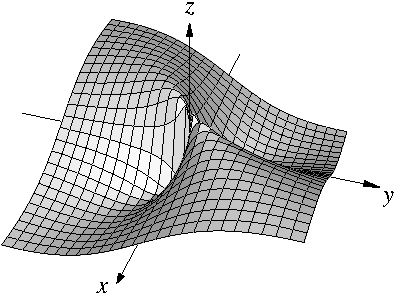
\includegraphics{figures/xyxsqysq}
\caption{Graph of $\frac{xy}{x^2+y^2}$.\label{fig:xyxsqysqvol2}}
\end{myfig}




%%%%%%%%%%%%%%%%%%%%%%%%%%%%%%%%%%%%%%%%%%%%%%%%%%%%%%%%%%%%%%%%%%%%%%%%%%%%%%
%%%%%%%%%%%%%%%%%%%%%%%%%%%%%%%%%%%%%%%%%%%%%%%%%%%%%%%%%%%%%%%%%%%%%%%%%%%%%%
%%%%%%%%%%%%%%%%%%%%%%%%%%%%%%%%%%%%%%%%%%%%%%%%%%%%%%%%%%%%%%%%%%%%%%%%%%%%%%

%FIXME: else I don't get links, weird
%\def\MR#1{\relax\ifhmode\unskip\spacefactor3000 \space\fi%
  %\href{http://www.ams.org/mathscinet-getitem?mr=#1}{MR#1}}
\def\myDOI#1{\href{http://dx.doi.org/#1}{#1}}



%FIXME
%\cleardoublepage  
\clearpage
\phantomsection
\addcontentsline{toc}{chapter}{Further reading}
\markboth{FURTHER READING}{FURTHER READING}
\begin{bibchapter}[Further Reading] \label{ch:furtherreading}

%Here we list useful books for extra reading.

\begin{biblist}[\normalsize]

%FIXME: also cite the ra book

\bib{ra:book}{misc}{
   author={Lebl, Ji\v{r}\'i},
   title={Basic Analysis I: Introduction to Real Analysis, Volume I},
   note={\url{https://www.jirka.org/ra/}}
}

\bib{ra:book2}{misc}{
   author={Lebl, Ji\v{r}\'i},
   title={Basic Analysis II: Introduction to Real Analysis, Volume II},
   note={\url{https://www.jirka.org/ra/}}
}

\bib{scv:book}{misc}{
   author={Lebl, Ji\v{r}\'i},
   title={Tasty bits of Several Complex Variables},
   note={\url{https://www.jirka.org/scv/}}
}

\bib{Rudin:principles}{book}{
   author={Rudin, Walter},
   title={Principles of mathematical analysis},
   edition={3},
   note={International Series in Pure and Applied Mathematics},
   publisher={McGraw-Hill Book Co., New York-Auckland-D\"usseldorf},
   date={1976},
   pages={x+342},
   review={\MR{0385023}},
}

\end{biblist}
\end{bibchapter}

%%%%%%%%%%%%%%%%%%%%%%%%%%%%%%%%%%%%%%%%%%%%%%%%%%%%%%%%%%%%%%%%%%%%%%%%%%%%%%
%%%%%%%%%%%%%%%%%%%%%%%%%%%%%%%%%%%%%%%%%%%%%%%%%%%%%%%%%%%%%%%%%%%%%%%%%%%%%%
%%%%%%%%%%%%%%%%%%%%%%%%%%%%%%%%%%%%%%%%%%%%%%%%%%%%%%%%%%%%%%%%%%%%%%%%%%%%%%

%\cleardoublepage  
\clearpage  
\phantomsection
\addcontentsline{toc}{chapter}{\indexname}  
\microtypesetup{protrusion=false}
\printindex
\microtypesetup{protrusion=true}

%%%%%%%%%%%%%%%%%%%%%%%%%%%%%%%%%%%%%%%%%%%%%%%%%%%%%%%%%%%%%%%%%%%%%%%%%%%%%%
%%%%%%%%%%%%%%%%%%%%%%%%%%%%%%%%%%%%%%%%%%%%%%%%%%%%%%%%%%%%%%%%%%%%%%%%%%%%%%
%%%%%%%%%%%%%%%%%%%%%%%%%%%%%%%%%%%%%%%%%%%%%%%%%%%%%%%%%%%%%%%%%%%%%%%%%%%%%%

%
% automake on glossaries doesn't work if the index is before the glossary.
% That's why the List of Notation is last, no other reason.  Problem is
% that printindex does a clearpage which screws up the delayed write18
% that glossaries sets up
%

\begingroup
\renewcommand{\pagelistname}{Page}
\setglossarystyle{long3colheader}
% correctly set up with cellspace
\renewenvironment{theglossary}%
  {\setlength\cellspacetoplimit{4pt}
   \setlength\cellspacebottomlimit{4pt}
   \setlength\LTleft{0pt}
   \setlength\LTright{0pt}
   \markboth{LIST OF NOTATION}{LIST OF NOTATION}
   \begin{longtable}{Sl @{\extracolsep{\fill}} Sl @{\extracolsep{\fill}} Sl}}%
  {\end{longtable}}%
\cleardoublepage
\microtypesetup{protrusion=false}
\printglossary[type=notation] 
\microtypesetup{protrusion=true}
\endgroup

\end{document}
